\documentclass[twoside]{book}

% Packages required by doxygen
\usepackage{fixltx2e}
\usepackage{calc}
\usepackage{doxygen}
\usepackage[export]{adjustbox} % also loads graphicx
\usepackage{graphicx}
\usepackage[utf8]{inputenc}
\usepackage{makeidx}
\usepackage{multicol}
\usepackage{multirow}
\PassOptionsToPackage{warn}{textcomp}
\usepackage{textcomp}
\usepackage[nointegrals]{wasysym}
\usepackage[table]{xcolor}

% Font selection
\usepackage[T1]{fontenc}
\usepackage[scaled=.90]{helvet}
\usepackage{courier}
\usepackage{amssymb}
\usepackage{sectsty}
\renewcommand{\familydefault}{\sfdefault}
\allsectionsfont{%
  \fontseries{bc}\selectfont%
  \color{darkgray}%
}
\renewcommand{\DoxyLabelFont}{%
  \fontseries{bc}\selectfont%
  \color{darkgray}%
}
\newcommand{\+}{\discretionary{\mbox{\scriptsize$\hookleftarrow$}}{}{}}

% Page & text layout
\usepackage{geometry}
\geometry{%
  a4paper,%
  top=2.5cm,%
  bottom=2.5cm,%
  left=2.5cm,%
  right=2.5cm%
}
\tolerance=750
\hfuzz=15pt
\hbadness=750
\setlength{\emergencystretch}{15pt}
\setlength{\parindent}{0cm}
\setlength{\parskip}{3ex plus 2ex minus 2ex}
\makeatletter
\renewcommand{\paragraph}{%
  \@startsection{paragraph}{4}{0ex}{-1.0ex}{1.0ex}{%
    \normalfont\normalsize\bfseries\SS@parafont%
  }%
}
\renewcommand{\subparagraph}{%
  \@startsection{subparagraph}{5}{0ex}{-1.0ex}{1.0ex}{%
    \normalfont\normalsize\bfseries\SS@subparafont%
  }%
}
\makeatother

% Headers & footers
\usepackage{fancyhdr}
\pagestyle{fancyplain}
\fancyhead[LE]{\fancyplain{}{\bfseries\thepage}}
\fancyhead[CE]{\fancyplain{}{}}
\fancyhead[RE]{\fancyplain{}{\bfseries\leftmark}}
\fancyhead[LO]{\fancyplain{}{\bfseries\rightmark}}
\fancyhead[CO]{\fancyplain{}{}}
\fancyhead[RO]{\fancyplain{}{\bfseries\thepage}}
\fancyfoot[LE]{\fancyplain{}{}}
\fancyfoot[CE]{\fancyplain{}{}}
\fancyfoot[RE]{\fancyplain{}{\bfseries\scriptsize Generated by Doxygen }}
\fancyfoot[LO]{\fancyplain{}{\bfseries\scriptsize Generated by Doxygen }}
\fancyfoot[CO]{\fancyplain{}{}}
\fancyfoot[RO]{\fancyplain{}{}}
\renewcommand{\footrulewidth}{0.4pt}
\renewcommand{\chaptermark}[1]{%
  \markboth{#1}{}%
}
\renewcommand{\sectionmark}[1]{%
  \markright{\thesection\ #1}%
}

% Indices & bibliography
\usepackage{natbib}
\usepackage[titles]{tocloft}
\setcounter{tocdepth}{3}
\setcounter{secnumdepth}{5}
\makeindex

% Hyperlinks (required, but should be loaded last)
\usepackage{ifpdf}
\ifpdf
  \usepackage[pdftex,pagebackref=true]{hyperref}
\else
  \usepackage[ps2pdf,pagebackref=true]{hyperref}
\fi
\hypersetup{%
  colorlinks=true,%
  linkcolor=blue,%
  citecolor=blue,%
  unicode%
}

% Custom commands
\newcommand{\clearemptydoublepage}{%
  \newpage{\pagestyle{empty}\cleardoublepage}%
}

\usepackage{caption}
\captionsetup{labelsep=space,justification=centering,font={bf},singlelinecheck=off,skip=4pt,position=top}

%===== C O N T E N T S =====

\begin{document}

% Titlepage & ToC
\hypersetup{pageanchor=false,
             bookmarksnumbered=true,
             pdfencoding=unicode
            }
\pagenumbering{alph}
\begin{titlepage}
\vspace*{7cm}
\begin{center}%
{\Large My Project }\\
\vspace*{1cm}
{\large Generated by Doxygen 1.8.13}\\
\end{center}
\end{titlepage}
\clearemptydoublepage
\pagenumbering{roman}
\tableofcontents
\clearemptydoublepage
\pagenumbering{arabic}
\hypersetup{pageanchor=true}

%--- Begin generated contents ---
\chapter{Class Index}
\section{Class List}
Here are the classes, structs, unions and interfaces with brief descriptions\+:\begin{DoxyCompactList}
\item\contentsline{section}{\hyperlink{structadd__entry}{add\+\_\+entry} }{\pageref{structadd__entry}}{}
\item\contentsline{section}{\hyperlink{structbuckets}{buckets} }{\pageref{structbuckets}}{}
\item\contentsline{section}{\hyperlink{structentry}{entry} }{\pageref{structentry}}{}
\item\contentsline{section}{\hyperlink{structentry__args}{entry\+\_\+args} }{\pageref{structentry__args}}{}
\item\contentsline{section}{\hyperlink{structhashmap__args}{hashmap\+\_\+args} }{\pageref{structhashmap__args}}{}
\item\contentsline{section}{\hyperlink{structhashmap__atomic}{hashmap\+\_\+atomic} }{\pageref{structhashmap__atomic}}{}
\item\contentsline{section}{\hyperlink{structhashmap__rp}{hashmap\+\_\+rp} }{\pageref{structhashmap__rp}}{}
\item\contentsline{section}{\hyperlink{structhashmap__tx}{hashmap\+\_\+tx} }{\pageref{structhashmap__tx}}{}
\end{DoxyCompactList}

\chapter{File Index}
\section{File List}
Here is a list of all documented files with brief descriptions\+:\begin{DoxyCompactList}
\item\contentsline{section}{\hyperlink{hashmap_8h}{hashmap.\+h} \\*Hashmap implementation in persistent memory }{\pageref{hashmap_8h}}{}
\item\contentsline{section}{\hyperlink{hashmap__atomic_8h}{hashmap\+\_\+atomic.\+h} \\*Implementation of atomic hashmap, where inserts are coordinated to be one after the other }{\pageref{hashmap__atomic_8h}}{}
\item\contentsline{section}{{\bfseries hashmap\+\_\+internal.\+h} }{\pageref{hashmap__internal_8h}}{}
\item\contentsline{section}{{\bfseries hashmap\+\_\+rp.\+h} }{\pageref{hashmap__rp_8h}}{}
\item\contentsline{section}{{\bfseries hashmap\+\_\+tx.\+h} }{\pageref{hashmap__tx_8h}}{}
\end{DoxyCompactList}

\chapter{Class Documentation}
\hypertarget{struct__art__leaf}{}\section{\+\_\+art\+\_\+leaf Struct Reference}
\label{struct__art__leaf}\index{\+\_\+art\+\_\+leaf@{\+\_\+art\+\_\+leaf}}


Collaboration diagram for \+\_\+art\+\_\+leaf\+:
% FIG 0
\subsection*{Public Member Functions}
\begin{DoxyCompactItemize}
\item 
\mbox{\Hypertarget{struct__art__leaf_a11e2deac1bcf5f88bb066a32351fe72c}\label{struct__art__leaf_a11e2deac1bcf5f88bb066a32351fe72c}} 
{\bfseries T\+O\+ID} (\hyperlink{struct__var__string}{var\+\_\+string}) value
\item 
\mbox{\Hypertarget{struct__art__leaf_a417bccd10d0c812fefaf1f435561a26a}\label{struct__art__leaf_a417bccd10d0c812fefaf1f435561a26a}} 
{\bfseries T\+O\+ID} (\hyperlink{struct__var__string}{var\+\_\+string}) key
\end{DoxyCompactItemize}
\subsection*{Public Attributes}
\begin{DoxyCompactItemize}
\item 
\mbox{\Hypertarget{struct__art__leaf_a3fc012976033db80eafceef0c304bd5a}\label{struct__art__leaf_a3fc012976033db80eafceef0c304bd5a}} 
union \hyperlink{union__toid__var__string__toid}{\+\_\+toid\+\_\+var\+\_\+string\+\_\+toid} {\bfseries value}
\item 
\mbox{\Hypertarget{struct__art__leaf_a1d867c7c6f1a06ad8a0ebf4b030a201d}\label{struct__art__leaf_a1d867c7c6f1a06ad8a0ebf4b030a201d}} 
union \hyperlink{union__toid__var__string__toid}{\+\_\+toid\+\_\+var\+\_\+string\+\_\+toid} {\bfseries key}
\end{DoxyCompactItemize}


The documentation for this struct was generated from the following files\+:\begin{DoxyCompactItemize}
\item 
libart/art.\+h\item 
libart/arttree\+\_\+structures.\+h\end{DoxyCompactItemize}

\hypertarget{struct__art__node}{}\section{\+\_\+art\+\_\+node Struct Reference}
\label{struct__art__node}\index{\+\_\+art\+\_\+node@{\+\_\+art\+\_\+node}}
\subsection*{Public Attributes}
\begin{DoxyCompactItemize}
\item 
\mbox{\Hypertarget{struct__art__node_a568c806ac46af5fd3872558ceb52038d}\label{struct__art__node_a568c806ac46af5fd3872558ceb52038d}} 
uint8\+\_\+t {\bfseries num\+\_\+children}
\item 
\mbox{\Hypertarget{struct__art__node_a7701e425f3817f5d747bd6dcc9b301ea}\label{struct__art__node_a7701e425f3817f5d747bd6dcc9b301ea}} 
uint32\+\_\+t {\bfseries partial\+\_\+len}
\item 
\mbox{\Hypertarget{struct__art__node_ad2fab3e7a29832c75b2bf8cfd1626799}\label{struct__art__node_ad2fab3e7a29832c75b2bf8cfd1626799}} 
unsigned char {\bfseries partial} \mbox{[}M\+A\+X\+\_\+\+P\+R\+E\+F\+I\+X\+\_\+\+L\+EN\mbox{]}
\end{DoxyCompactItemize}


The documentation for this struct was generated from the following files\+:\begin{DoxyCompactItemize}
\item 
libart/art.\+h\item 
libart/arttree\+\_\+structures.\+h\end{DoxyCompactItemize}

\hypertarget{struct__art__node16}{}\section{\+\_\+art\+\_\+node16 Struct Reference}
\label{struct__art__node16}\index{\+\_\+art\+\_\+node16@{\+\_\+art\+\_\+node16}}


Collaboration diagram for \+\_\+art\+\_\+node16\+:
% FIG 0
\subsection*{Public Member Functions}
\begin{DoxyCompactItemize}
\item 
\mbox{\Hypertarget{struct__art__node16_a94c28b57dd8cc192ec20756e78cb8c89}\label{struct__art__node16_a94c28b57dd8cc192ec20756e78cb8c89}} 
{\bfseries T\+O\+ID} (\hyperlink{struct__art__node__u}{art\+\_\+node\+\_\+u}) children\mbox{[}16\mbox{]}
\end{DoxyCompactItemize}
\subsection*{Public Attributes}
\begin{DoxyCompactItemize}
\item 
\mbox{\Hypertarget{struct__art__node16_afae26149cdfd134b5ded76b7e4fab889}\label{struct__art__node16_afae26149cdfd134b5ded76b7e4fab889}} 
\hyperlink{struct__art__node}{art\+\_\+node} {\bfseries n}
\item 
\mbox{\Hypertarget{struct__art__node16_a2df42019d4a87b03eb0331a309497247}\label{struct__art__node16_a2df42019d4a87b03eb0331a309497247}} 
unsigned char {\bfseries keys} \mbox{[}16\mbox{]}
\item 
\mbox{\Hypertarget{struct__art__node16_a231efc93632d538fb3ab3134dde8f194}\label{struct__art__node16_a231efc93632d538fb3ab3134dde8f194}} 
union \hyperlink{union__toid__art__node__u__toid}{\+\_\+toid\+\_\+art\+\_\+node\+\_\+u\+\_\+toid} {\bfseries children} \mbox{[}16\mbox{]}
\end{DoxyCompactItemize}


The documentation for this struct was generated from the following files\+:\begin{DoxyCompactItemize}
\item 
libart/art.\+h\item 
libart/arttree\+\_\+structures.\+h\end{DoxyCompactItemize}

\hypertarget{struct__art__node256}{}\section{\+\_\+art\+\_\+node256 Struct Reference}
\label{struct__art__node256}\index{\+\_\+art\+\_\+node256@{\+\_\+art\+\_\+node256}}


Collaboration diagram for \+\_\+art\+\_\+node256\+:
% FIG 0
\subsection*{Public Member Functions}
\begin{DoxyCompactItemize}
\item 
\mbox{\Hypertarget{struct__art__node256_a944164248d2f74ef56471c1db080c7ca}\label{struct__art__node256_a944164248d2f74ef56471c1db080c7ca}} 
{\bfseries T\+O\+ID} (\hyperlink{struct__art__node__u}{art\+\_\+node\+\_\+u}) children\mbox{[}256\mbox{]}
\end{DoxyCompactItemize}
\subsection*{Public Attributes}
\begin{DoxyCompactItemize}
\item 
\mbox{\Hypertarget{struct__art__node256_a3226feced4b9d35d11a25582827a0b98}\label{struct__art__node256_a3226feced4b9d35d11a25582827a0b98}} 
\hyperlink{struct__art__node}{art\+\_\+node} {\bfseries n}
\item 
\mbox{\Hypertarget{struct__art__node256_a3d58086b3e06c83ae35e6304e4d1df9e}\label{struct__art__node256_a3d58086b3e06c83ae35e6304e4d1df9e}} 
union \hyperlink{union__toid__art__node__u__toid}{\+\_\+toid\+\_\+art\+\_\+node\+\_\+u\+\_\+toid} {\bfseries children} \mbox{[}256\mbox{]}
\end{DoxyCompactItemize}


The documentation for this struct was generated from the following files\+:\begin{DoxyCompactItemize}
\item 
libart/art.\+h\item 
libart/arttree\+\_\+structures.\+h\end{DoxyCompactItemize}

\hypertarget{struct__art__node4}{}\section{\+\_\+art\+\_\+node4 Struct Reference}
\label{struct__art__node4}\index{\+\_\+art\+\_\+node4@{\+\_\+art\+\_\+node4}}


Collaboration diagram for \+\_\+art\+\_\+node4\+:
% FIG 0
\subsection*{Public Member Functions}
\begin{DoxyCompactItemize}
\item 
\mbox{\Hypertarget{struct__art__node4_a4bdf49c0fa04557a729c3cd976d5c607}\label{struct__art__node4_a4bdf49c0fa04557a729c3cd976d5c607}} 
{\bfseries T\+O\+ID} (\hyperlink{struct__art__node__u}{art\+\_\+node\+\_\+u}) children\mbox{[}4\mbox{]}
\end{DoxyCompactItemize}
\subsection*{Public Attributes}
\begin{DoxyCompactItemize}
\item 
\mbox{\Hypertarget{struct__art__node4_a0415ddf340cef55b6dbf6449666b47d8}\label{struct__art__node4_a0415ddf340cef55b6dbf6449666b47d8}} 
\hyperlink{struct__art__node}{art\+\_\+node} {\bfseries n}
\item 
\mbox{\Hypertarget{struct__art__node4_ac46521df7b3fe39ccef684639590ce11}\label{struct__art__node4_ac46521df7b3fe39ccef684639590ce11}} 
unsigned char {\bfseries keys} \mbox{[}4\mbox{]}
\item 
\mbox{\Hypertarget{struct__art__node4_a25f2d86c7c050ef4922ca8e6354550e3}\label{struct__art__node4_a25f2d86c7c050ef4922ca8e6354550e3}} 
union \hyperlink{union__toid__art__node__u__toid}{\+\_\+toid\+\_\+art\+\_\+node\+\_\+u\+\_\+toid} {\bfseries children} \mbox{[}4\mbox{]}
\end{DoxyCompactItemize}


The documentation for this struct was generated from the following files\+:\begin{DoxyCompactItemize}
\item 
libart/art.\+h\item 
libart/arttree\+\_\+structures.\+h\end{DoxyCompactItemize}

\hypertarget{struct__art__node48}{}\section{\+\_\+art\+\_\+node48 Struct Reference}
\label{struct__art__node48}\index{\+\_\+art\+\_\+node48@{\+\_\+art\+\_\+node48}}


Collaboration diagram for \+\_\+art\+\_\+node48\+:
% FIG 0
\subsection*{Public Member Functions}
\begin{DoxyCompactItemize}
\item 
\mbox{\Hypertarget{struct__art__node48_af13c73d4484e7cc3c0c27cd35ab5e76b}\label{struct__art__node48_af13c73d4484e7cc3c0c27cd35ab5e76b}} 
{\bfseries T\+O\+ID} (\hyperlink{struct__art__node__u}{art\+\_\+node\+\_\+u}) children\mbox{[}48\mbox{]}
\end{DoxyCompactItemize}
\subsection*{Public Attributes}
\begin{DoxyCompactItemize}
\item 
\mbox{\Hypertarget{struct__art__node48_aec3337c7cb130d838bddef718e6927fd}\label{struct__art__node48_aec3337c7cb130d838bddef718e6927fd}} 
\hyperlink{struct__art__node}{art\+\_\+node} {\bfseries n}
\item 
\mbox{\Hypertarget{struct__art__node48_a254fad0f2d7d7a085322fb699b220ce3}\label{struct__art__node48_a254fad0f2d7d7a085322fb699b220ce3}} 
unsigned char {\bfseries keys} \mbox{[}256\mbox{]}
\item 
\mbox{\Hypertarget{struct__art__node48_a4490f2fe3bbc7b2403e452d14042e8b2}\label{struct__art__node48_a4490f2fe3bbc7b2403e452d14042e8b2}} 
union \hyperlink{union__toid__art__node__u__toid}{\+\_\+toid\+\_\+art\+\_\+node\+\_\+u\+\_\+toid} {\bfseries children} \mbox{[}48\mbox{]}
\end{DoxyCompactItemize}


The documentation for this struct was generated from the following files\+:\begin{DoxyCompactItemize}
\item 
libart/art.\+h\item 
libart/arttree\+\_\+structures.\+h\end{DoxyCompactItemize}

\hypertarget{struct__art__node__u}{}\section{\+\_\+art\+\_\+node\+\_\+u Struct Reference}
\label{struct__art__node__u}\index{\+\_\+art\+\_\+node\+\_\+u@{\+\_\+art\+\_\+node\+\_\+u}}


Collaboration diagram for \+\_\+art\+\_\+node\+\_\+u\+:
% FIG 0
\subsection*{Public Attributes}
\begin{DoxyCompactItemize}
\item 
\mbox{\Hypertarget{struct__art__node__u_a7a307683078edd5e38b8aa14a783393f}\label{struct__art__node__u_a7a307683078edd5e38b8aa14a783393f}} 
uint8\+\_\+t {\bfseries art\+\_\+node\+\_\+type}
\item 
\mbox{\Hypertarget{struct__art__node__u_ae36910ced1e3012676429e15b6e41991}\label{struct__art__node__u_ae36910ced1e3012676429e15b6e41991}} 
uint8\+\_\+t {\bfseries art\+\_\+node\+\_\+tag}
\item 
\mbox{\Hypertarget{struct__art__node__u_a457159e1eb7a00a0b939936f087b9f26}\label{struct__art__node__u_a457159e1eb7a00a0b939936f087b9f26}} 
\begin{tabbing}
xx\=xx\=xx\=xx\=xx\=xx\=xx\=xx\=xx\=\kill
union \{\\
\} {\bfseries u}\\

\end{tabbing}\item 
\mbox{\Hypertarget{struct__art__node__u_a9511a898c16de6c671d511d8f2c33d9d}\label{struct__art__node__u_a9511a898c16de6c671d511d8f2c33d9d}} 
\begin{tabbing}
xx\=xx\=xx\=xx\=xx\=xx\=xx\=xx\=xx\=\kill
union \{\\
\>union \hyperlink{union__toid__art__node4__toid}{\_toid\_art\_node4\_toid} {\bfseries an4}\\
\>union \hyperlink{union__toid__art__node16__toid}{\_toid\_art\_node16\_toid} {\bfseries an16}\\
\>union \hyperlink{union__toid__art__node48__toid}{\_toid\_art\_node48\_toid} {\bfseries an48}\\
\>union \hyperlink{union__toid__art__node256__toid}{\_toid\_art\_node256\_toid} {\bfseries an256}\\
\>union \hyperlink{union__toid__art__leaf__toid}{\_toid\_art\_leaf\_toid} {\bfseries al}\\
\} {\bfseries u}\\

\end{tabbing}\end{DoxyCompactItemize}


The documentation for this struct was generated from the following files\+:\begin{DoxyCompactItemize}
\item 
libart/art.\+h\item 
libart/arttree\+\_\+structures.\+h\end{DoxyCompactItemize}

\hypertarget{struct__art__tree__root}{}\section{\+\_\+art\+\_\+tree\+\_\+root Struct Reference}
\label{struct__art__tree__root}\index{\+\_\+art\+\_\+tree\+\_\+root@{\+\_\+art\+\_\+tree\+\_\+root}}


Collaboration diagram for \+\_\+art\+\_\+tree\+\_\+root\+:
% FIG 0
\subsection*{Public Attributes}
\begin{DoxyCompactItemize}
\item 
\mbox{\Hypertarget{struct__art__tree__root_aca717aef2b7622c34beb35a5fde6f00f}\label{struct__art__tree__root_aca717aef2b7622c34beb35a5fde6f00f}} 
int {\bfseries size}
\item 
\mbox{\Hypertarget{struct__art__tree__root_a33cff6a7215f0a112cb96266673c9b99}\label{struct__art__tree__root_a33cff6a7215f0a112cb96266673c9b99}} 
union \hyperlink{union__toid__art__node__u__toid}{\+\_\+toid\+\_\+art\+\_\+node\+\_\+u\+\_\+toid} {\bfseries root}
\end{DoxyCompactItemize}


The documentation for this struct was generated from the following file\+:\begin{DoxyCompactItemize}
\item 
libart/arttree\+\_\+structures.\+h\end{DoxyCompactItemize}

\hypertarget{struct__cb__data}{}\section{\+\_\+cb\+\_\+data Struct Reference}
\label{struct__cb__data}\index{\+\_\+cb\+\_\+data@{\+\_\+cb\+\_\+data}}
\subsection*{Public Member Functions}
\begin{DoxyCompactItemize}
\item 
\mbox{\Hypertarget{struct__cb__data_a52c41acd51a4a1a8daea2fc414b603b0}\label{struct__cb__data_a52c41acd51a4a1a8daea2fc414b603b0}} 
{\bfseries T\+O\+ID} (\hyperlink{struct__art__node__u}{art\+\_\+node\+\_\+u}) node
\end{DoxyCompactItemize}
\subsection*{Public Attributes}
\begin{DoxyCompactItemize}
\item 
\mbox{\Hypertarget{struct__cb__data_a77ba76da523cea6b7be15af27db8488d}\label{struct__cb__data_a77ba76da523cea6b7be15af27db8488d}} 
int {\bfseries child\+\_\+idx}
\end{DoxyCompactItemize}


The documentation for this struct was generated from the following file\+:\begin{DoxyCompactItemize}
\item 
libart/art.\+h\end{DoxyCompactItemize}

\hypertarget{union__toid__art__leaf__toid}{}\section{\+\_\+toid\+\_\+art\+\_\+leaf\+\_\+toid Union Reference}
\label{union__toid__art__leaf__toid}\index{\+\_\+toid\+\_\+art\+\_\+leaf\+\_\+toid@{\+\_\+toid\+\_\+art\+\_\+leaf\+\_\+toid}}


Collaboration diagram for \+\_\+toid\+\_\+art\+\_\+leaf\+\_\+toid\+:
% FIG 0
\subsection*{Public Attributes}
\begin{DoxyCompactItemize}
\item 
\mbox{\Hypertarget{union__toid__art__leaf__toid_a9d1049b2118c67e31a5b677feec8e690}\label{union__toid__art__leaf__toid_a9d1049b2118c67e31a5b677feec8e690}} 
\hyperlink{structpmemoid}{P\+M\+E\+Moid} {\bfseries oid}
\item 
\mbox{\Hypertarget{union__toid__art__leaf__toid_a4b5bc6854e369c59d6695219efb69156}\label{union__toid__art__leaf__toid_a4b5bc6854e369c59d6695219efb69156}} 
\hyperlink{struct__art__leaf}{art\+\_\+leaf} $\ast$ {\bfseries \+\_\+type}
\item 
\mbox{\Hypertarget{union__toid__art__leaf__toid_abf8bfa16199858dc92f318525faa9b99}\label{union__toid__art__leaf__toid_abf8bfa16199858dc92f318525faa9b99}} 
\+\_\+toid\+\_\+art\+\_\+leaf\+\_\+toid\+\_\+type\+\_\+num $\ast$ {\bfseries \+\_\+type\+\_\+num}
\end{DoxyCompactItemize}


The documentation for this union was generated from the following file\+:\begin{DoxyCompactItemize}
\item 
libart/arttree\+\_\+structures.\+h\end{DoxyCompactItemize}

\hypertarget{union__toid__art__node16__toid}{}\section{\+\_\+toid\+\_\+art\+\_\+node16\+\_\+toid Union Reference}
\label{union__toid__art__node16__toid}\index{\+\_\+toid\+\_\+art\+\_\+node16\+\_\+toid@{\+\_\+toid\+\_\+art\+\_\+node16\+\_\+toid}}


Collaboration diagram for \+\_\+toid\+\_\+art\+\_\+node16\+\_\+toid\+:
% FIG 0
\subsection*{Public Attributes}
\begin{DoxyCompactItemize}
\item 
\mbox{\Hypertarget{union__toid__art__node16__toid_a72853d970e703c4a024b7de9614a9589}\label{union__toid__art__node16__toid_a72853d970e703c4a024b7de9614a9589}} 
\hyperlink{structpmemoid}{P\+M\+E\+Moid} {\bfseries oid}
\item 
\mbox{\Hypertarget{union__toid__art__node16__toid_a814d7a03678b76b5213db57e0b6594a0}\label{union__toid__art__node16__toid_a814d7a03678b76b5213db57e0b6594a0}} 
\hyperlink{struct__art__node16}{art\+\_\+node16} $\ast$ {\bfseries \+\_\+type}
\item 
\mbox{\Hypertarget{union__toid__art__node16__toid_a612bf95789db93865838ac2ac74c837b}\label{union__toid__art__node16__toid_a612bf95789db93865838ac2ac74c837b}} 
\+\_\+toid\+\_\+art\+\_\+node16\+\_\+toid\+\_\+type\+\_\+num $\ast$ {\bfseries \+\_\+type\+\_\+num}
\end{DoxyCompactItemize}


The documentation for this union was generated from the following file\+:\begin{DoxyCompactItemize}
\item 
libart/arttree\+\_\+structures.\+h\end{DoxyCompactItemize}

\hypertarget{union__toid__art__node256__toid}{}\section{\+\_\+toid\+\_\+art\+\_\+node256\+\_\+toid Union Reference}
\label{union__toid__art__node256__toid}\index{\+\_\+toid\+\_\+art\+\_\+node256\+\_\+toid@{\+\_\+toid\+\_\+art\+\_\+node256\+\_\+toid}}


Collaboration diagram for \+\_\+toid\+\_\+art\+\_\+node256\+\_\+toid\+:
% FIG 0
\subsection*{Public Attributes}
\begin{DoxyCompactItemize}
\item 
\mbox{\Hypertarget{union__toid__art__node256__toid_a7898a9dd528bdce7e7651f1506b16543}\label{union__toid__art__node256__toid_a7898a9dd528bdce7e7651f1506b16543}} 
\hyperlink{structpmemoid}{P\+M\+E\+Moid} {\bfseries oid}
\item 
\mbox{\Hypertarget{union__toid__art__node256__toid_a23062c2ac99316afea6387d6ef2aefe1}\label{union__toid__art__node256__toid_a23062c2ac99316afea6387d6ef2aefe1}} 
\hyperlink{struct__art__node256}{art\+\_\+node256} $\ast$ {\bfseries \+\_\+type}
\item 
\mbox{\Hypertarget{union__toid__art__node256__toid_a21beeaaf99ff16a30ced4344b6069783}\label{union__toid__art__node256__toid_a21beeaaf99ff16a30ced4344b6069783}} 
\+\_\+toid\+\_\+art\+\_\+node256\+\_\+toid\+\_\+type\+\_\+num $\ast$ {\bfseries \+\_\+type\+\_\+num}
\end{DoxyCompactItemize}


The documentation for this union was generated from the following file\+:\begin{DoxyCompactItemize}
\item 
libart/arttree\+\_\+structures.\+h\end{DoxyCompactItemize}

\hypertarget{union__toid__art__node48__toid}{}\section{\+\_\+toid\+\_\+art\+\_\+node48\+\_\+toid Union Reference}
\label{union__toid__art__node48__toid}\index{\+\_\+toid\+\_\+art\+\_\+node48\+\_\+toid@{\+\_\+toid\+\_\+art\+\_\+node48\+\_\+toid}}


Collaboration diagram for \+\_\+toid\+\_\+art\+\_\+node48\+\_\+toid\+:
% FIG 0
\subsection*{Public Attributes}
\begin{DoxyCompactItemize}
\item 
\mbox{\Hypertarget{union__toid__art__node48__toid_a0489ea7eb3c98660ca61834892a0ffdb}\label{union__toid__art__node48__toid_a0489ea7eb3c98660ca61834892a0ffdb}} 
\hyperlink{structpmemoid}{P\+M\+E\+Moid} {\bfseries oid}
\item 
\mbox{\Hypertarget{union__toid__art__node48__toid_a2760e4109502625dacca967a36f78a70}\label{union__toid__art__node48__toid_a2760e4109502625dacca967a36f78a70}} 
\hyperlink{struct__art__node48}{art\+\_\+node48} $\ast$ {\bfseries \+\_\+type}
\item 
\mbox{\Hypertarget{union__toid__art__node48__toid_a032f85b0270a114961ebf818378e5dbe}\label{union__toid__art__node48__toid_a032f85b0270a114961ebf818378e5dbe}} 
\+\_\+toid\+\_\+art\+\_\+node48\+\_\+toid\+\_\+type\+\_\+num $\ast$ {\bfseries \+\_\+type\+\_\+num}
\end{DoxyCompactItemize}


The documentation for this union was generated from the following file\+:\begin{DoxyCompactItemize}
\item 
libart/arttree\+\_\+structures.\+h\end{DoxyCompactItemize}

\hypertarget{union__toid__art__node4__toid}{}\section{\+\_\+toid\+\_\+art\+\_\+node4\+\_\+toid Union Reference}
\label{union__toid__art__node4__toid}\index{\+\_\+toid\+\_\+art\+\_\+node4\+\_\+toid@{\+\_\+toid\+\_\+art\+\_\+node4\+\_\+toid}}


Collaboration diagram for \+\_\+toid\+\_\+art\+\_\+node4\+\_\+toid\+:
% FIG 0
\subsection*{Public Attributes}
\begin{DoxyCompactItemize}
\item 
\mbox{\Hypertarget{union__toid__art__node4__toid_ac67b41cac00f0dab21789fbc0327239a}\label{union__toid__art__node4__toid_ac67b41cac00f0dab21789fbc0327239a}} 
\hyperlink{structpmemoid}{P\+M\+E\+Moid} {\bfseries oid}
\item 
\mbox{\Hypertarget{union__toid__art__node4__toid_ab874dc090bde73feec5a4598f2638904}\label{union__toid__art__node4__toid_ab874dc090bde73feec5a4598f2638904}} 
\hyperlink{struct__art__node4}{art\+\_\+node4} $\ast$ {\bfseries \+\_\+type}
\item 
\mbox{\Hypertarget{union__toid__art__node4__toid_a5b560202123e55019ebc6cf73a4a18fe}\label{union__toid__art__node4__toid_a5b560202123e55019ebc6cf73a4a18fe}} 
\+\_\+toid\+\_\+art\+\_\+node4\+\_\+toid\+\_\+type\+\_\+num $\ast$ {\bfseries \+\_\+type\+\_\+num}
\end{DoxyCompactItemize}


The documentation for this union was generated from the following file\+:\begin{DoxyCompactItemize}
\item 
libart/arttree\+\_\+structures.\+h\end{DoxyCompactItemize}

\hypertarget{union__toid__art__node__toid}{}\section{\+\_\+toid\+\_\+art\+\_\+node\+\_\+toid Union Reference}
\label{union__toid__art__node__toid}\index{\+\_\+toid\+\_\+art\+\_\+node\+\_\+toid@{\+\_\+toid\+\_\+art\+\_\+node\+\_\+toid}}


Collaboration diagram for \+\_\+toid\+\_\+art\+\_\+node\+\_\+toid\+:
% FIG 0
\subsection*{Public Attributes}
\begin{DoxyCompactItemize}
\item 
\mbox{\Hypertarget{union__toid__art__node__toid_af3026cc97b4fe7114534e1e6c0896daf}\label{union__toid__art__node__toid_af3026cc97b4fe7114534e1e6c0896daf}} 
\hyperlink{structpmemoid}{P\+M\+E\+Moid} {\bfseries oid}
\item 
\mbox{\Hypertarget{union__toid__art__node__toid_ad6bd05d91d8c56112ce388d405d618ca}\label{union__toid__art__node__toid_ad6bd05d91d8c56112ce388d405d618ca}} 
\hyperlink{struct__art__node}{art\+\_\+node} $\ast$ {\bfseries \+\_\+type}
\item 
\mbox{\Hypertarget{union__toid__art__node__toid_af8584f1221c5eda9977a7f1ebbe919ad}\label{union__toid__art__node__toid_af8584f1221c5eda9977a7f1ebbe919ad}} 
\+\_\+toid\+\_\+art\+\_\+node\+\_\+toid\+\_\+type\+\_\+num $\ast$ {\bfseries \+\_\+type\+\_\+num}
\end{DoxyCompactItemize}


The documentation for this union was generated from the following file\+:\begin{DoxyCompactItemize}
\item 
libart/arttree\+\_\+structures.\+h\end{DoxyCompactItemize}

\hypertarget{union__toid__art__node__u__toid}{}\section{\+\_\+toid\+\_\+art\+\_\+node\+\_\+u\+\_\+toid Union Reference}
\label{union__toid__art__node__u__toid}\index{\+\_\+toid\+\_\+art\+\_\+node\+\_\+u\+\_\+toid@{\+\_\+toid\+\_\+art\+\_\+node\+\_\+u\+\_\+toid}}


Collaboration diagram for \+\_\+toid\+\_\+art\+\_\+node\+\_\+u\+\_\+toid\+:
% FIG 0
\subsection*{Public Attributes}
\begin{DoxyCompactItemize}
\item 
\mbox{\Hypertarget{union__toid__art__node__u__toid_a323252c64266a12bf8264142c516e2e6}\label{union__toid__art__node__u__toid_a323252c64266a12bf8264142c516e2e6}} 
\hyperlink{structpmemoid}{P\+M\+E\+Moid} {\bfseries oid}
\item 
\mbox{\Hypertarget{union__toid__art__node__u__toid_a805554574c1ec52470c33064aba288de}\label{union__toid__art__node__u__toid_a805554574c1ec52470c33064aba288de}} 
\hyperlink{struct__art__node__u}{art\+\_\+node\+\_\+u} $\ast$ {\bfseries \+\_\+type}
\item 
\mbox{\Hypertarget{union__toid__art__node__u__toid_ae443c287aef941d81ea066bf8f0db413}\label{union__toid__art__node__u__toid_ae443c287aef941d81ea066bf8f0db413}} 
\+\_\+toid\+\_\+art\+\_\+node\+\_\+u\+\_\+toid\+\_\+type\+\_\+num $\ast$ {\bfseries \+\_\+type\+\_\+num}
\end{DoxyCompactItemize}


The documentation for this union was generated from the following file\+:\begin{DoxyCompactItemize}
\item 
libart/arttree\+\_\+structures.\+h\end{DoxyCompactItemize}

\hypertarget{union__toid__var__string__toid}{}\section{\+\_\+toid\+\_\+var\+\_\+string\+\_\+toid Union Reference}
\label{union__toid__var__string__toid}\index{\+\_\+toid\+\_\+var\+\_\+string\+\_\+toid@{\+\_\+toid\+\_\+var\+\_\+string\+\_\+toid}}


Collaboration diagram for \+\_\+toid\+\_\+var\+\_\+string\+\_\+toid\+:
% FIG 0
\subsection*{Public Attributes}
\begin{DoxyCompactItemize}
\item 
\mbox{\Hypertarget{union__toid__var__string__toid_a8a367ef9c8c3610112991d68c036bc69}\label{union__toid__var__string__toid_a8a367ef9c8c3610112991d68c036bc69}} 
\hyperlink{structpmemoid}{P\+M\+E\+Moid} {\bfseries oid}
\item 
\mbox{\Hypertarget{union__toid__var__string__toid_ac1b22352535d5b9c8b0f6daa4639da50}\label{union__toid__var__string__toid_ac1b22352535d5b9c8b0f6daa4639da50}} 
\hyperlink{struct__var__string}{var\+\_\+string} $\ast$ {\bfseries \+\_\+type}
\item 
\mbox{\Hypertarget{union__toid__var__string__toid_a6d7a023cecc5aa9c161d5373d2f1bc20}\label{union__toid__var__string__toid_a6d7a023cecc5aa9c161d5373d2f1bc20}} 
\+\_\+toid\+\_\+var\+\_\+string\+\_\+toid\+\_\+type\+\_\+num $\ast$ {\bfseries \+\_\+type\+\_\+num}
\end{DoxyCompactItemize}


The documentation for this union was generated from the following file\+:\begin{DoxyCompactItemize}
\item 
libart/arttree\+\_\+structures.\+h\end{DoxyCompactItemize}

\hypertarget{struct__var__string}{}\section{\+\_\+var\+\_\+string Struct Reference}
\label{struct__var__string}\index{\+\_\+var\+\_\+string@{\+\_\+var\+\_\+string}}
\subsection*{Public Attributes}
\begin{DoxyCompactItemize}
\item 
\mbox{\Hypertarget{struct__var__string_aefb53479fd422ce6cd457cf7e57eba19}\label{struct__var__string_aefb53479fd422ce6cd457cf7e57eba19}} 
size\+\_\+t {\bfseries len}
\item 
\mbox{\Hypertarget{struct__var__string_a112aa22cf4b6eea009bb02a1d5e8b6a1}\label{struct__var__string_a112aa22cf4b6eea009bb02a1d5e8b6a1}} 
unsigned char {\bfseries s} \mbox{[}$\,$\mbox{]}
\end{DoxyCompactItemize}


The documentation for this struct was generated from the following files\+:\begin{DoxyCompactItemize}
\item 
libart/art.\+h\item 
libart/arttree\+\_\+structures.\+h\end{DoxyCompactItemize}

\hypertarget{structadd__entry}{}\section{add\+\_\+entry Struct Reference}
\label{structadd__entry}\index{add\+\_\+entry@{add\+\_\+entry}}


Collaboration diagram for add\+\_\+entry\+:
% FIG 0
\subsection*{Public Attributes}
\begin{DoxyCompactItemize}
\item 
\mbox{\Hypertarget{structadd__entry_ada303ac47bbd298d31a08ff5fb0c8d48}\label{structadd__entry_ada303ac47bbd298d31a08ff5fb0c8d48}} 
struct \hyperlink{structentry}{entry} {\bfseries data}
\item 
\mbox{\Hypertarget{structadd__entry_aff20888396f928a47207ec2fe432efe9}\label{structadd__entry_aff20888396f928a47207ec2fe432efe9}} 
size\+\_\+t {\bfseries pos}
\item 
\mbox{\Hypertarget{structadd__entry_a02a8967aa6cd3e8bbbaa6c35571379a2}\label{structadd__entry_a02a8967aa6cd3e8bbbaa6c35571379a2}} 
struct pobj\+\_\+action $\ast$ {\bfseries actv}
\item 
\mbox{\Hypertarget{structadd__entry_a288eb722a38cd8a357d0600475defe70}\label{structadd__entry_a288eb722a38cd8a357d0600475defe70}} 
size\+\_\+t {\bfseries actv\+\_\+cnt}
\end{DoxyCompactItemize}


The documentation for this struct was generated from the following file\+:\begin{DoxyCompactItemize}
\item 
hashmap/hashmap\+\_\+rp.\+c\end{DoxyCompactItemize}

\hypertarget{structalien}{}\section{alien Struct Reference}
\label{structalien}\index{alien@{alien}}
\subsection*{Public Attributes}
\begin{DoxyCompactItemize}
\item 
\mbox{\Hypertarget{structalien_ad1a54b0957f6532b94fe028803546b18}\label{structalien_ad1a54b0957f6532b94fe028803546b18}} 
uint16\+\_\+t {\bfseries x}
\item 
\mbox{\Hypertarget{structalien_a4df242edfb1ab274c812a78f76e2836e}\label{structalien_a4df242edfb1ab274c812a78f76e2836e}} 
uint16\+\_\+t {\bfseries y}
\item 
\mbox{\Hypertarget{structalien_a72f3950d108ca416266ef6b109cd189a}\label{structalien_a72f3950d108ca416266ef6b109cd189a}} 
uint32\+\_\+t {\bfseries timer}
\item 
\mbox{\Hypertarget{structalien_a36d07156cb4c40f731e58ca2bd38b282}\label{structalien_a36d07156cb4c40f731e58ca2bd38b282}} 
unsigned {\bfseries x}
\item 
\mbox{\Hypertarget{structalien_a81d3961b661d01b590151a3e9eb00b08}\label{structalien_a81d3961b661d01b590151a3e9eb00b08}} 
unsigned {\bfseries y}
\end{DoxyCompactItemize}


The documentation for this struct was generated from the following files\+:\begin{DoxyCompactItemize}
\item 
pminvaders/pminvaders.\+c\item 
pminvaders/pminvaders2.\+c\end{DoxyCompactItemize}

\hypertarget{structarray__elm}{}\section{array\+\_\+elm Struct Reference}
\label{structarray__elm}\index{array\+\_\+elm@{array\+\_\+elm}}
\subsection*{Public Attributes}
\begin{DoxyCompactItemize}
\item 
\mbox{\Hypertarget{structarray__elm_a2b4f75b5ca99d2c6fea1793585395094}\label{structarray__elm_a2b4f75b5ca99d2c6fea1793585395094}} 
int {\bfseries id}
\end{DoxyCompactItemize}


The documentation for this struct was generated from the following file\+:\begin{DoxyCompactItemize}
\item 
array/array.\+c\end{DoxyCompactItemize}

\hypertarget{structarray__info}{}\section{array\+\_\+info Struct Reference}
\label{structarray__info}\index{array\+\_\+info@{array\+\_\+info}}


Collaboration diagram for array\+\_\+info\+:
% FIG 0
\subsection*{Public Attributes}
\begin{DoxyCompactItemize}
\item 
\mbox{\Hypertarget{structarray__info_ae785f8b874daaf0bb1d8d92857f163bd}\label{structarray__info_ae785f8b874daaf0bb1d8d92857f163bd}} 
char {\bfseries name} \mbox{[}M\+A\+X\+\_\+\+B\+U\+F\+F\+L\+EN\mbox{]}
\item 
\mbox{\Hypertarget{structarray__info_a636917523226311ab337778e594b6dfe}\label{structarray__info_a636917523226311ab337778e594b6dfe}} 
size\+\_\+t {\bfseries size}
\item 
\mbox{\Hypertarget{structarray__info_ab7e20da6f960cb6a3066dc09b776c1e1}\label{structarray__info_ab7e20da6f960cb6a3066dc09b776c1e1}} 
enum array\+\_\+types {\bfseries type}
\item 
\mbox{\Hypertarget{structarray__info_a9782c68cc4bcbe037d6dd94abc767a99}\label{structarray__info_a9782c68cc4bcbe037d6dd94abc767a99}} 
\hyperlink{structpmemoid}{P\+M\+E\+Moid} {\bfseries array}
\end{DoxyCompactItemize}


The documentation for this struct was generated from the following file\+:\begin{DoxyCompactItemize}
\item 
array/array.\+c\end{DoxyCompactItemize}

\hypertarget{structart__tree__root}{}\section{art\+\_\+tree\+\_\+root Struct Reference}
\label{structart__tree__root}\index{art\+\_\+tree\+\_\+root@{art\+\_\+tree\+\_\+root}}
\subsection*{Public Member Functions}
\begin{DoxyCompactItemize}
\item 
\mbox{\Hypertarget{structart__tree__root_a2bbd25a5cc17e803418d9963fef257cf}\label{structart__tree__root_a2bbd25a5cc17e803418d9963fef257cf}} 
{\bfseries T\+O\+ID} (\hyperlink{struct__art__node__u}{art\+\_\+node\+\_\+u}) \hyperlink{structroot}{root}
\end{DoxyCompactItemize}
\subsection*{Public Attributes}
\begin{DoxyCompactItemize}
\item 
\mbox{\Hypertarget{structart__tree__root_a400af60db816e51e1f02df9f0d9b345d}\label{structart__tree__root_a400af60db816e51e1f02df9f0d9b345d}} 
int {\bfseries size}
\end{DoxyCompactItemize}


The documentation for this struct was generated from the following file\+:\begin{DoxyCompactItemize}
\item 
libart/art.\+h\end{DoxyCompactItemize}

\hypertarget{unionart__tree__root__toid}{}\section{art\+\_\+tree\+\_\+root\+\_\+toid Union Reference}
\label{unionart__tree__root__toid}\index{art\+\_\+tree\+\_\+root\+\_\+toid@{art\+\_\+tree\+\_\+root\+\_\+toid}}


Collaboration diagram for art\+\_\+tree\+\_\+root\+\_\+toid\+:
% FIG 0
\subsection*{Public Attributes}
\begin{DoxyCompactItemize}
\item 
\mbox{\Hypertarget{unionart__tree__root__toid_a7bcb9827ffb1979a1ee1fe984b04e1ce}\label{unionart__tree__root__toid_a7bcb9827ffb1979a1ee1fe984b04e1ce}} 
\hyperlink{structpmemoid}{P\+M\+E\+Moid} {\bfseries oid}
\item 
\mbox{\Hypertarget{unionart__tree__root__toid_aef2521da5feb66bb0f14adb765149b78}\label{unionart__tree__root__toid_aef2521da5feb66bb0f14adb765149b78}} 
struct \hyperlink{structart__tree__root}{art\+\_\+tree\+\_\+root} $\ast$ {\bfseries \+\_\+type}
\item 
\mbox{\Hypertarget{unionart__tree__root__toid_ac15d2068d1e5e3d5abc20cc8a9d19fdb}\label{unionart__tree__root__toid_ac15d2068d1e5e3d5abc20cc8a9d19fdb}} 
art\+\_\+tree\+\_\+root\+\_\+toid\+\_\+type\+\_\+num $\ast$ {\bfseries \+\_\+type\+\_\+num}
\end{DoxyCompactItemize}


The documentation for this union was generated from the following file\+:\begin{DoxyCompactItemize}
\item 
libart/arttree\+\_\+structures.\+h\end{DoxyCompactItemize}

\hypertarget{structbar}{}\section{bar Struct Reference}
\label{structbar}\index{bar@{bar}}
\subsection*{Public Attributes}
\begin{DoxyCompactItemize}
\item 
\mbox{\Hypertarget{structbar_a1ffba8508191d82c82990fc3ed2172b2}\label{structbar_a1ffba8508191d82c82990fc3ed2172b2}} 
char {\bfseries data} \mbox{[}500\mbox{]}
\end{DoxyCompactItemize}


The documentation for this struct was generated from the following file\+:\begin{DoxyCompactItemize}
\item 
slab\+\_\+allocator/main.\+c\end{DoxyCompactItemize}

\hypertarget{structbar__el}{}\section{bar\+\_\+el Struct Reference}
\label{structbar__el}\index{bar\+\_\+el@{bar\+\_\+el}}


The documentation for this struct was generated from the following file\+:\begin{DoxyCompactItemize}
\item 
lists.\+c\end{DoxyCompactItemize}

\hypertarget{structbase}{}\section{base Struct Reference}
\label{structbase}\index{base@{base}}


Collaboration diagram for base\+:
% FIG 0
\subsection*{Public Attributes}
\begin{DoxyCompactItemize}
\item 
\mbox{\Hypertarget{structbase_a204b27012357fc5a2389ce6af2af0bbf}\label{structbase_a204b27012357fc5a2389ce6af2af0bbf}} 
\hyperlink{structpmemoid}{P\+M\+E\+Moid} {\bfseries head}
\item 
\mbox{\Hypertarget{structbase_ae3620a9af489aff396d1a0e95579c3b2}\label{structbase_ae3620a9af489aff396d1a0e95579c3b2}} 
\hyperlink{structpmemoid}{P\+M\+E\+Moid} {\bfseries tail}
\item 
\mbox{\Hypertarget{structbase_a48d3f088327acf89a409f764f0c08d30}\label{structbase_a48d3f088327acf89a409f764f0c08d30}} 
P\+M\+E\+Mrwlock {\bfseries rwlock}
\item 
\mbox{\Hypertarget{structbase_a1380b4faf8053707a83425210f03b8c8}\label{structbase_a1380b4faf8053707a83425210f03b8c8}} 
size\+\_\+t {\bfseries bytes\+\_\+written}
\end{DoxyCompactItemize}


The documentation for this struct was generated from the following files\+:\begin{DoxyCompactItemize}
\item 
pmemblk/obj\+\_\+pmemblk.\+c\item 
pmemlog/obj\+\_\+pmemlog.\+c\item 
pmemlog/obj\+\_\+pmemlog\+\_\+simple.\+c\end{DoxyCompactItemize}

\hypertarget{structbtree}{}\section{btree Struct Reference}
\label{structbtree}\index{btree@{btree}}


The documentation for this struct was generated from the following file\+:\begin{DoxyCompactItemize}
\item 
btree.\+c\end{DoxyCompactItemize}

\hypertarget{structbtree__map}{}\section{btree\+\_\+map Struct Reference}
\label{structbtree__map}\index{btree\+\_\+map@{btree\+\_\+map}}


The documentation for this struct was generated from the following file\+:\begin{DoxyCompactItemize}
\item 
tree\+\_\+map/btree\+\_\+map.\+c\end{DoxyCompactItemize}

\hypertarget{structbtree__node}{}\section{btree\+\_\+node Struct Reference}
\label{structbtree__node}\index{btree\+\_\+node@{btree\+\_\+node}}
\subsection*{Public Attributes}
\begin{DoxyCompactItemize}
\item 
\mbox{\Hypertarget{structbtree__node_ae9807c6d556e3443d00a86881b193254}\label{structbtree__node_ae9807c6d556e3443d00a86881b193254}} 
int64\+\_\+t {\bfseries key}
\end{DoxyCompactItemize}


The documentation for this struct was generated from the following file\+:\begin{DoxyCompactItemize}
\item 
btree.\+c\end{DoxyCompactItemize}

\hypertarget{structbtree__node__arg}{}\section{btree\+\_\+node\+\_\+arg Struct Reference}
\label{structbtree__node__arg}\index{btree\+\_\+node\+\_\+arg@{btree\+\_\+node\+\_\+arg}}
\subsection*{Public Attributes}
\begin{DoxyCompactItemize}
\item 
\mbox{\Hypertarget{structbtree__node__arg_a14eb6fbb08477cefc15bac2da4c765f8}\label{structbtree__node__arg_a14eb6fbb08477cefc15bac2da4c765f8}} 
size\+\_\+t {\bfseries size}
\item 
\mbox{\Hypertarget{structbtree__node__arg_a3ef0f2b80b73a149700358a717799428}\label{structbtree__node__arg_a3ef0f2b80b73a149700358a717799428}} 
int64\+\_\+t {\bfseries key}
\item 
\mbox{\Hypertarget{structbtree__node__arg_a6732e14a29d800e8ccae2e700b93bca5}\label{structbtree__node__arg_a6732e14a29d800e8ccae2e700b93bca5}} 
const char $\ast$ {\bfseries value}
\end{DoxyCompactItemize}


The documentation for this struct was generated from the following file\+:\begin{DoxyCompactItemize}
\item 
btree.\+c\end{DoxyCompactItemize}

\hypertarget{structbuckets}{}\section{buckets Struct Reference}
\label{structbuckets}\index{buckets@{buckets}}
\subsection*{Public Attributes}
\begin{DoxyCompactItemize}
\item 
\mbox{\Hypertarget{structbuckets_ab4b1efc42ff06fef401feb5297469441}\label{structbuckets_ab4b1efc42ff06fef401feb5297469441}} 
size\+\_\+t {\bfseries nbuckets}
\item 
\mbox{\Hypertarget{structbuckets_a563609796b380211a16c9f0eb07c4ff6}\label{structbuckets_a563609796b380211a16c9f0eb07c4ff6}} 
struct entries\+\_\+head {\bfseries bucket} \mbox{[}$\,$\mbox{]}
\end{DoxyCompactItemize}


The documentation for this struct was generated from the following files\+:\begin{DoxyCompactItemize}
\item 
hashmap/hashmap\+\_\+atomic.\+c\item 
hashmap/hashmap\+\_\+tx.\+c\end{DoxyCompactItemize}

\hypertarget{structbullet}{}\section{bullet Struct Reference}
\label{structbullet}\index{bullet@{bullet}}
\subsection*{Public Attributes}
\begin{DoxyCompactItemize}
\item 
\mbox{\Hypertarget{structbullet_a5a8ecfe86933fad2966d1184a04761bc}\label{structbullet_a5a8ecfe86933fad2966d1184a04761bc}} 
uint16\+\_\+t {\bfseries x}
\item 
\mbox{\Hypertarget{structbullet_a18437e1768cfa3c7ad25f8e05eecaa2a}\label{structbullet_a18437e1768cfa3c7ad25f8e05eecaa2a}} 
uint16\+\_\+t {\bfseries y}
\item 
\mbox{\Hypertarget{structbullet_a7c980430c22b07baef1df11a472eb3b4}\label{structbullet_a7c980430c22b07baef1df11a472eb3b4}} 
uint32\+\_\+t {\bfseries timer}
\item 
\mbox{\Hypertarget{structbullet_a2b17fdd1d92d937134ef029ee0eb84b3}\label{structbullet_a2b17fdd1d92d937134ef029ee0eb84b3}} 
unsigned {\bfseries x}
\item 
\mbox{\Hypertarget{structbullet_ab001bd7da16e0748f2f6847690ce170f}\label{structbullet_ab001bd7da16e0748f2f6847690ce170f}} 
unsigned {\bfseries y}
\item 
\mbox{\Hypertarget{structbullet_a421e5c55a10cd48e4598c9f761e77b0c}\label{structbullet_a421e5c55a10cd48e4598c9f761e77b0c}} 
unsigned {\bfseries timer}
\end{DoxyCompactItemize}


The documentation for this struct was generated from the following files\+:\begin{DoxyCompactItemize}
\item 
pminvaders/pminvaders.\+c\item 
pminvaders/pminvaders2.\+c\end{DoxyCompactItemize}

\hypertarget{structcb__arg2}{}\section{cb\+\_\+arg2 Struct Reference}
\label{structcb__arg2}\index{cb\+\_\+arg2@{cb\+\_\+arg2}}
\subsection*{Public Attributes}
\begin{DoxyCompactItemize}
\item 
\mbox{\Hypertarget{structcb__arg2_a33ba5dab65addea38de54263bbf24f04}\label{structcb__arg2_a33ba5dab65addea38de54263bbf24f04}} 
int($\ast$ {\bfseries cb} )(uint64\+\_\+t key, \hyperlink{structpmemoid}{P\+M\+E\+Moid} value, void $\ast$arg)
\item 
\mbox{\Hypertarget{structcb__arg2_a64dc721d857d7e8272620a348f79911e}\label{structcb__arg2_a64dc721d857d7e8272620a348f79911e}} 
void $\ast$ {\bfseries arg}
\end{DoxyCompactItemize}


The documentation for this struct was generated from the following file\+:\begin{DoxyCompactItemize}
\item 
map/map\+\_\+rtree.\+c\end{DoxyCompactItemize}

\hypertarget{structclient__data}{}\section{client\+\_\+data Struct Reference}
\label{structclient__data}\index{client\+\_\+data@{client\+\_\+data}}
\subsection*{Public Attributes}
\begin{DoxyCompactItemize}
\item 
\mbox{\Hypertarget{structclient__data_a11add7cdbb8e257ef6fe3aca3be4e157}\label{structclient__data_a11add7cdbb8e257ef6fe3aca3be4e157}} 
char $\ast$ {\bfseries buf}
\item 
\mbox{\Hypertarget{structclient__data_a03747a1317ed2159a3f685f8f4688961}\label{structclient__data_a03747a1317ed2159a3f685f8f4688961}} 
size\+\_\+t {\bfseries buf\+\_\+len}
\item 
\mbox{\Hypertarget{structclient__data_a5df0c8ac8973c66f5b436f7549eb6cb3}\label{structclient__data_a5df0c8ac8973c66f5b436f7549eb6cb3}} 
size\+\_\+t {\bfseries len}
\end{DoxyCompactItemize}


The documentation for this struct was generated from the following file\+:\begin{DoxyCompactItemize}
\item 
map/kv\+\_\+server.\+c\end{DoxyCompactItemize}

\hypertarget{structcommand}{}\section{command Struct Reference}
\label{structcommand}\index{command@{command}}
\subsection*{Public Attributes}
\begin{DoxyCompactItemize}
\item 
\mbox{\Hypertarget{structcommand_abe8e2307ef5e2b469ce227af336b3a78}\label{structcommand_abe8e2307ef5e2b469ce227af336b3a78}} 
const char $\ast$ {\bfseries name}
\item 
\mbox{\Hypertarget{structcommand_a9eebac54783247ee795dc7e6196240bd}\label{structcommand_a9eebac54783247ee795dc7e6196240bd}} 
const char $\ast$ {\bfseries brief}
\item 
\mbox{\Hypertarget{structcommand_a0021992c3299e1d70188894548f51b58}\label{structcommand_a0021992c3299e1d70188894548f51b58}} 
int($\ast$ {\bfseries func} )(char $\ast$, struct \hyperlink{structpmem__context}{pmem\+\_\+context} $\ast$, int, char $\ast$\mbox{[}$\,$\mbox{]})
\item 
\mbox{\Hypertarget{structcommand_a43ee7e284b376499a99a5fa2d4905e92}\label{structcommand_a43ee7e284b376499a99a5fa2d4905e92}} 
void($\ast$ {\bfseries help} )(char $\ast$)
\end{DoxyCompactItemize}


The documentation for this struct was generated from the following file\+:\begin{DoxyCompactItemize}
\item 
libart/arttree\+\_\+structures.\+c\end{DoxyCompactItemize}

\hypertarget{structcreate__args}{}\section{create\+\_\+args Struct Reference}
\label{structcreate__args}\index{create\+\_\+args@{create\+\_\+args}}
\subsection*{Public Attributes}
\begin{DoxyCompactItemize}
\item 
\mbox{\Hypertarget{structcreate__args_add64a085a263209d88311956f30ca8e0}\label{structcreate__args_add64a085a263209d88311956f30ca8e0}} 
size\+\_\+t {\bfseries size}
\item 
\mbox{\Hypertarget{structcreate__args_aa725c2d8040c1e66935265bf692f3fe1}\label{structcreate__args_aa725c2d8040c1e66935265bf692f3fe1}} 
const void $\ast$ {\bfseries src}
\end{DoxyCompactItemize}


The documentation for this struct was generated from the following file\+:\begin{DoxyCompactItemize}
\item 
pmemlog/obj\+\_\+pmemlog\+\_\+minimal.\+c\end{DoxyCompactItemize}

\hypertarget{structctree__map}{}\section{ctree\+\_\+map Struct Reference}
\label{structctree__map}\index{ctree\+\_\+map@{ctree\+\_\+map}}


Collaboration diagram for ctree\+\_\+map\+:
% FIG 0
\subsection*{Public Attributes}
\begin{DoxyCompactItemize}
\item 
\mbox{\Hypertarget{structctree__map_ab50b235f435c07650d2834c078f3fcff}\label{structctree__map_ab50b235f435c07650d2834c078f3fcff}} 
struct \hyperlink{structtree__map__entry}{tree\+\_\+map\+\_\+entry} {\bfseries root}
\end{DoxyCompactItemize}


The documentation for this struct was generated from the following file\+:\begin{DoxyCompactItemize}
\item 
tree\+\_\+map/ctree\+\_\+map.\+c\end{DoxyCompactItemize}

\hypertarget{structdatastore}{}\section{datastore Struct Reference}
\label{structdatastore}\index{datastore@{datastore}}
\subsection*{Public Attributes}
\begin{DoxyCompactItemize}
\item 
\mbox{\Hypertarget{structdatastore_a7acbd30899b87641a3cae41289a50367}\label{structdatastore_a7acbd30899b87641a3cae41289a50367}} 
void $\ast$ {\bfseries priv}
\end{DoxyCompactItemize}


The documentation for this struct was generated from the following file\+:\begin{DoxyCompactItemize}
\item 
libart/arttree.\+c\end{DoxyCompactItemize}

\hypertarget{structds__context}{}\section{ds\+\_\+context Struct Reference}
\label{structds__context}\index{ds\+\_\+context@{ds\+\_\+context}}
\subsection*{Public Attributes}
\begin{DoxyCompactItemize}
\item 
\mbox{\Hypertarget{structds__context_a164c6d00c66a6fa48729b3c709aa4dd5}\label{structds__context_a164c6d00c66a6fa48729b3c709aa4dd5}} 
char $\ast$ {\bfseries filename}
\item 
\mbox{\Hypertarget{structds__context_a26b599f2639d5ba6fd571f7deb438039}\label{structds__context_a26b599f2639d5ba6fd571f7deb438039}} 
int {\bfseries mode}
\item 
\mbox{\Hypertarget{structds__context_ab72d2cc9cbab07fede0e65c0c7b37d10}\label{structds__context_ab72d2cc9cbab07fede0e65c0c7b37d10}} 
int {\bfseries insertions}
\item 
\mbox{\Hypertarget{structds__context_a527716230aa63398a8dade8029f0649c}\label{structds__context_a527716230aa63398a8dade8029f0649c}} 
int {\bfseries newpool}
\item 
\mbox{\Hypertarget{structds__context_a2d82a7eb4e13a9841bf55199fabd706f}\label{structds__context_a2d82a7eb4e13a9841bf55199fabd706f}} 
size\+\_\+t {\bfseries psize}
\item 
\mbox{\Hypertarget{structds__context_ac2c635639cf5495e7b0ce4b82659146a}\label{structds__context_ac2c635639cf5495e7b0ce4b82659146a}} 
P\+M\+E\+Mobjpool $\ast$ {\bfseries pop}
\item 
\mbox{\Hypertarget{structds__context_a0ec463e2fa6e543aad41d0a6d12b9971}\label{structds__context_a0ec463e2fa6e543aad41d0a6d12b9971}} 
bool {\bfseries fileio}
\item 
\mbox{\Hypertarget{structds__context_a322561a4c870afa684a1c38159dfe8d4}\label{structds__context_a322561a4c870afa684a1c38159dfe8d4}} 
unsigned {\bfseries fmode}
\item 
\mbox{\Hypertarget{structds__context_acd1582bade589b6f66d9b2e0b915da39}\label{structds__context_acd1582bade589b6f66d9b2e0b915da39}} 
int {\bfseries fd}
\item 
\mbox{\Hypertarget{structds__context_a6d9cec34cd6854d2c53383a2218cd3cc}\label{structds__context_a6d9cec34cd6854d2c53383a2218cd3cc}} 
char $\ast$ {\bfseries addr}
\item 
\mbox{\Hypertarget{structds__context_af14f4e7f3e6ae0275d364664e0eb74a6}\label{structds__context_af14f4e7f3e6ae0275d364664e0eb74a6}} 
unsigned char $\ast$ {\bfseries key}
\item 
\mbox{\Hypertarget{structds__context_af60f306c9195616aaa574e0302603eab}\label{structds__context_af60f306c9195616aaa574e0302603eab}} 
uint32\+\_\+t {\bfseries key\+\_\+len}
\item 
\mbox{\Hypertarget{structds__context_a40c875f0541182e528d26d5bbc8ec5f2}\label{structds__context_a40c875f0541182e528d26d5bbc8ec5f2}} 
unsigned char $\ast$ {\bfseries value}
\item 
\mbox{\Hypertarget{structds__context_abb6d28824cc5c5bd3effecdc8a902489}\label{structds__context_abb6d28824cc5c5bd3effecdc8a902489}} 
uint32\+\_\+t {\bfseries val\+\_\+len}
\end{DoxyCompactItemize}


The documentation for this struct was generated from the following file\+:\begin{DoxyCompactItemize}
\item 
libart/arttree.\+c\end{DoxyCompactItemize}

\hypertarget{structentry}{}\section{entry Struct Reference}
\label{structentry}\index{entry@{entry}}


Collaboration diagram for entry\+:
% FIG 0
\subsection*{Public Attributes}
\begin{DoxyCompactItemize}
\item 
\mbox{\Hypertarget{structentry_a9baabf5b8c35d0a925340cd73e23ae8d}\label{structentry_a9baabf5b8c35d0a925340cd73e23ae8d}} 
uint64\+\_\+t {\bfseries key}
\item 
\mbox{\Hypertarget{structentry_abc6a75d6690199042034e9300aebd4c1}\label{structentry_abc6a75d6690199042034e9300aebd4c1}} 
\hyperlink{structpmemoid}{P\+M\+E\+Moid} {\bfseries value}
\item 
\mbox{\Hypertarget{structentry_a97cd1dbcdcea14e94f70a86a391b662b}\label{structentry_a97cd1dbcdcea14e94f70a86a391b662b}} 
uint64\+\_\+t {\bfseries hash}
\item 
\mbox{\Hypertarget{structentry_a8ac9b199255dffa2da0510ee7f85c4e4}\label{structentry_a8ac9b199255dffa2da0510ee7f85c4e4}} 
size\+\_\+t {\bfseries len}
\item 
\mbox{\Hypertarget{structentry_aaf5d81a7428014e8bb4711f33ff134eb}\label{structentry_aaf5d81a7428014e8bb4711f33ff134eb}} 
char {\bfseries data} \mbox{[}$\,$\mbox{]}
\end{DoxyCompactItemize}


The documentation for this struct was generated from the following files\+:\begin{DoxyCompactItemize}
\item 
hashmap/hashmap\+\_\+atomic.\+c\item 
hashmap/hashmap\+\_\+rp.\+c\item 
hashmap/hashmap\+\_\+tx.\+c\item 
queue/queue.\+c\end{DoxyCompactItemize}

\hypertarget{structentry__args}{}\section{entry\+\_\+args Struct Reference}
\label{structentry__args}\index{entry\+\_\+args@{entry\+\_\+args}}
\subsection*{Public Attributes}
\begin{DoxyCompactItemize}
\item 
uint64\+\_\+t {\bfseries key}\hypertarget{structentry__args_aba46158e3af0f0f4701ea742f7e05697}{}\label{structentry__args_aba46158e3af0f0f4701ea742f7e05697}

\item 
P\+M\+E\+Moid {\bfseries value}\hypertarget{structentry__args_a8a910e88fcd1bb7d94aa52080d6abb08}{}\label{structentry__args_a8a910e88fcd1bb7d94aa52080d6abb08}

\end{DoxyCompactItemize}


The documentation for this struct was generated from the following file\+:\begin{DoxyCompactItemize}
\item 
hashmap\+\_\+atomic.\+c\end{DoxyCompactItemize}

\hypertarget{structexamine}{}\section{examine Struct Reference}
\label{structexamine}\index{examine@{examine}}
\subsection*{Public Attributes}
\begin{DoxyCompactItemize}
\item 
\mbox{\Hypertarget{structexamine_ae505057d5627be07305b251125bee3ee}\label{structexamine_ae505057d5627be07305b251125bee3ee}} 
const char $\ast$ {\bfseries name}
\item 
\mbox{\Hypertarget{structexamine_a67ca25732b457f0dd3aef7d33eaea243}\label{structexamine_a67ca25732b457f0dd3aef7d33eaea243}} 
const char $\ast$ {\bfseries brief}
\item 
\mbox{\Hypertarget{structexamine_a2acd23e70fd92a66bef62c02076f2095}\label{structexamine_a2acd23e70fd92a66bef62c02076f2095}} 
int($\ast$ {\bfseries func} )(char $\ast$, struct \hyperlink{structexamine__ctx}{examine\+\_\+ctx} $\ast$, off\+\_\+t)
\item 
\mbox{\Hypertarget{structexamine_a755e6e20a4997cd7c1f568fabc56867c}\label{structexamine_a755e6e20a4997cd7c1f568fabc56867c}} 
void($\ast$ {\bfseries help} )(char $\ast$)
\end{DoxyCompactItemize}


The documentation for this struct was generated from the following file\+:\begin{DoxyCompactItemize}
\item 
libart/arttree\+\_\+examine.\+c\end{DoxyCompactItemize}

\hypertarget{structexamine__ctx}{}\section{examine\+\_\+ctx Struct Reference}
\label{structexamine__ctx}\index{examine\+\_\+ctx@{examine\+\_\+ctx}}


Collaboration diagram for examine\+\_\+ctx\+:
% FIG 0
\subsection*{Public Attributes}
\begin{DoxyCompactItemize}
\item 
\mbox{\Hypertarget{structexamine__ctx_a3fbc6138bd215b73904626ba1e00ba7d}\label{structexamine__ctx_a3fbc6138bd215b73904626ba1e00ba7d}} 
struct \hyperlink{structpmem__context}{pmem\+\_\+context} $\ast$ {\bfseries pmem\+\_\+ctx}
\item 
\mbox{\Hypertarget{structexamine__ctx_abbcea7810c58839ecf6561f23a47e063}\label{structexamine__ctx_abbcea7810c58839ecf6561f23a47e063}} 
char $\ast$ {\bfseries offset\+\_\+string}
\item 
\mbox{\Hypertarget{structexamine__ctx_a596b7f4ec335d61033c5110f555acc36}\label{structexamine__ctx_a596b7f4ec335d61033c5110f555acc36}} 
uint64\+\_\+t {\bfseries offset}
\item 
\mbox{\Hypertarget{structexamine__ctx_a85c40b081b19ae7dcbdcca4f97746935}\label{structexamine__ctx_a85c40b081b19ae7dcbdcca4f97746935}} 
char $\ast$ {\bfseries type\+\_\+name}
\item 
\mbox{\Hypertarget{structexamine__ctx_a577989f9998f6b30313299e8d9b33665}\label{structexamine__ctx_a577989f9998f6b30313299e8d9b33665}} 
int32\+\_\+t {\bfseries type}
\item 
\mbox{\Hypertarget{structexamine__ctx_a06b7f7e343eca90dc385ec7e0a222aa4}\label{structexamine__ctx_a06b7f7e343eca90dc385ec7e0a222aa4}} 
int32\+\_\+t {\bfseries hexdump}
\end{DoxyCompactItemize}


The documentation for this struct was generated from the following file\+:\begin{DoxyCompactItemize}
\item 
libart/arttree\+\_\+examine.\+c\end{DoxyCompactItemize}

\hypertarget{structfifo__root}{}\section{fifo\+\_\+root Struct Reference}
\label{structfifo__root}\index{fifo\+\_\+root@{fifo\+\_\+root}}
\subsection*{Public Attributes}
\begin{DoxyCompactItemize}
\item 
\mbox{\Hypertarget{structfifo__root_aa377ffaa3f82aee9f7a51ecb2c520f84}\label{structfifo__root_aa377ffaa3f82aee9f7a51ecb2c520f84}} 
struct tqueuehead {\bfseries head}
\end{DoxyCompactItemize}


\subsection{Detailed Description}
Indication of the F\+I\+FO root node or the head node of the tqueue 

The documentation for this struct was generated from the following file\+:\begin{DoxyCompactItemize}
\item 
linkedlist/\hyperlink{fifo_8c}{fifo.\+c}\end{DoxyCompactItemize}

\hypertarget{structfoo}{}\section{foo Struct Reference}
\label{structfoo}\index{foo@{foo}}
\subsection*{Public Attributes}
\begin{DoxyCompactItemize}
\item 
\mbox{\Hypertarget{structfoo_a4f0cb361d81b7343369aacb13d4b1a6b}\label{structfoo_a4f0cb361d81b7343369aacb13d4b1a6b}} 
char {\bfseries data} \mbox{[}100\mbox{]}
\end{DoxyCompactItemize}


The documentation for this struct was generated from the following file\+:\begin{DoxyCompactItemize}
\item 
slab\+\_\+allocator/main.\+c\end{DoxyCompactItemize}

\hypertarget{structfoo__el}{}\section{foo\+\_\+el Struct Reference}
\label{structfoo__el}\index{foo\+\_\+el@{foo\+\_\+el}}


The documentation for this struct was generated from the following file\+:\begin{DoxyCompactItemize}
\item 
lists.\+c\end{DoxyCompactItemize}

\hypertarget{structgame__state}{}\section{game\+\_\+state Struct Reference}
\label{structgame__state}\index{game\+\_\+state@{game\+\_\+state}}
\subsection*{Public Attributes}
\begin{DoxyCompactItemize}
\item 
\mbox{\Hypertarget{structgame__state_aadb7591ec27de3807447e28973a100d4}\label{structgame__state_aadb7591ec27de3807447e28973a100d4}} 
uint32\+\_\+t {\bfseries timer}
\item 
\mbox{\Hypertarget{structgame__state_ae8bb405815b2ba7cc4e645dfdfb44aec}\label{structgame__state_ae8bb405815b2ba7cc4e645dfdfb44aec}} 
uint16\+\_\+t {\bfseries score}
\item 
\mbox{\Hypertarget{structgame__state_ac43d75a328259837d14b9c1ad6ee1bf0}\label{structgame__state_ac43d75a328259837d14b9c1ad6ee1bf0}} 
uint16\+\_\+t {\bfseries high\+\_\+score}
\end{DoxyCompactItemize}


The documentation for this struct was generated from the following file\+:\begin{DoxyCompactItemize}
\item 
pminvaders/pminvaders.\+c\end{DoxyCompactItemize}

\hypertarget{structhashmap__args}{}\section{hashmap\+\_\+args Struct Reference}
\label{structhashmap__args}\index{hashmap\+\_\+args@{hashmap\+\_\+args}}
\subsection*{Public Attributes}
\begin{DoxyCompactItemize}
\item 
uint32\+\_\+t {\bfseries seed}\hypertarget{structhashmap__args_ae512628a8f83e3c1fca257201607b529}{}\label{structhashmap__args_ae512628a8f83e3c1fca257201607b529}

\end{DoxyCompactItemize}


The documentation for this struct was generated from the following file\+:\begin{DoxyCompactItemize}
\item 
\hyperlink{hashmap_8h}{hashmap.\+h}\end{DoxyCompactItemize}

\hypertarget{structhashmap__atomic}{}\section{hashmap\+\_\+atomic Struct Reference}
\label{structhashmap__atomic}\index{hashmap\+\_\+atomic@{hashmap\+\_\+atomic}}
\subsection*{Public Attributes}
\begin{DoxyCompactItemize}
\item 
\mbox{\Hypertarget{structhashmap__atomic_a83e3b765935189ca4a6bf0c0e33c8d09}\label{structhashmap__atomic_a83e3b765935189ca4a6bf0c0e33c8d09}} 
uint32\+\_\+t {\bfseries seed}
\item 
\mbox{\Hypertarget{structhashmap__atomic_a95d74f846934cb275183a28df0ff14a8}\label{structhashmap__atomic_a95d74f846934cb275183a28df0ff14a8}} 
uint32\+\_\+t {\bfseries hash\+\_\+fun\+\_\+a}
\item 
\mbox{\Hypertarget{structhashmap__atomic_aa2476a3fa7d4d13c4b4d83d80ee1bb4c}\label{structhashmap__atomic_aa2476a3fa7d4d13c4b4d83d80ee1bb4c}} 
uint32\+\_\+t {\bfseries hash\+\_\+fun\+\_\+b}
\item 
\mbox{\Hypertarget{structhashmap__atomic_ae9459faea29e49b192e2c2d8e59d235d}\label{structhashmap__atomic_ae9459faea29e49b192e2c2d8e59d235d}} 
uint64\+\_\+t {\bfseries hash\+\_\+fun\+\_\+p}
\item 
\mbox{\Hypertarget{structhashmap__atomic_adb45831ae8cc7d5335b048ccc0ba2009}\label{structhashmap__atomic_adb45831ae8cc7d5335b048ccc0ba2009}} 
uint64\+\_\+t {\bfseries count}
\item 
\mbox{\Hypertarget{structhashmap__atomic_a4e9b4e9443278085568203af85278e6f}\label{structhashmap__atomic_a4e9b4e9443278085568203af85278e6f}} 
uint32\+\_\+t {\bfseries count\+\_\+dirty}
\end{DoxyCompactItemize}


The documentation for this struct was generated from the following file\+:\begin{DoxyCompactItemize}
\item 
hashmap/hashmap\+\_\+atomic.\+c\end{DoxyCompactItemize}

\hypertarget{structhashmap__rp}{}\section{hashmap\+\_\+rp Struct Reference}
\label{structhashmap__rp}\index{hashmap\+\_\+rp@{hashmap\+\_\+rp}}
\subsection*{Public Attributes}
\begin{DoxyCompactItemize}
\item 
uint64\+\_\+t {\bfseries count}\hypertarget{structhashmap__rp_ab6c1dfb752de6101545bb92dcccc419a}{}\label{structhashmap__rp_ab6c1dfb752de6101545bb92dcccc419a}

\item 
uint64\+\_\+t {\bfseries capacity}\hypertarget{structhashmap__rp_a964fc2490d30dc7a73328999f7759076}{}\label{structhashmap__rp_a964fc2490d30dc7a73328999f7759076}

\item 
uint64\+\_\+t {\bfseries resize\+\_\+threshold}\hypertarget{structhashmap__rp_afcf78d28515e6c63cddd440e5b02c79c}{}\label{structhashmap__rp_afcf78d28515e6c63cddd440e5b02c79c}

\end{DoxyCompactItemize}


The documentation for this struct was generated from the following file\+:\begin{DoxyCompactItemize}
\item 
hashmap\+\_\+rp.\+c\end{DoxyCompactItemize}

\hypertarget{structhashmap__tx}{}\section{hashmap\+\_\+tx Struct Reference}
\label{structhashmap__tx}\index{hashmap\+\_\+tx@{hashmap\+\_\+tx}}
\subsection*{Public Attributes}
\begin{DoxyCompactItemize}
\item 
uint32\+\_\+t {\bfseries seed}\hypertarget{structhashmap__tx_a3a3693aa60920c724a0f4511b18a6fd2}{}\label{structhashmap__tx_a3a3693aa60920c724a0f4511b18a6fd2}

\item 
uint32\+\_\+t {\bfseries hash\+\_\+fun\+\_\+a}\hypertarget{structhashmap__tx_aff7708436836d0ae87500fa876dfcecf}{}\label{structhashmap__tx_aff7708436836d0ae87500fa876dfcecf}

\item 
uint32\+\_\+t {\bfseries hash\+\_\+fun\+\_\+b}\hypertarget{structhashmap__tx_a9f6c8ffb7a4f3472edb7afeb99e45074}{}\label{structhashmap__tx_a9f6c8ffb7a4f3472edb7afeb99e45074}

\item 
uint64\+\_\+t {\bfseries hash\+\_\+fun\+\_\+p}\hypertarget{structhashmap__tx_adc5b9769a040542bda4f25e3098f2837}{}\label{structhashmap__tx_adc5b9769a040542bda4f25e3098f2837}

\item 
uint64\+\_\+t {\bfseries count}\hypertarget{structhashmap__tx_a70fbb5e277e0e52c199c1024cfbd08c1}{}\label{structhashmap__tx_a70fbb5e277e0e52c199c1024cfbd08c1}

\end{DoxyCompactItemize}


The documentation for this struct was generated from the following file\+:\begin{DoxyCompactItemize}
\item 
hashmap\+\_\+tx.\+c\end{DoxyCompactItemize}

\hypertarget{structlist__constr__args}{}\section{list\+\_\+constr\+\_\+args Struct Reference}
\label{structlist__constr__args}\index{list\+\_\+constr\+\_\+args@{list\+\_\+constr\+\_\+args}}
\subsection*{Public Attributes}
\begin{DoxyCompactItemize}
\item 
\mbox{\Hypertarget{structlist__constr__args_abf60829ebf7a89e6ca637b3111ce02c8}\label{structlist__constr__args_abf60829ebf7a89e6ca637b3111ce02c8}} 
enum list\+\_\+type {\bfseries type}
\item 
\mbox{\Hypertarget{structlist__constr__args_a19d03d2b8142d311c66314b405c7555d}\label{structlist__constr__args_a19d03d2b8142d311c66314b405c7555d}} 
int {\bfseries value}
\end{DoxyCompactItemize}


The documentation for this struct was generated from the following file\+:\begin{DoxyCompactItemize}
\item 
lists.\+c\end{DoxyCompactItemize}

\hypertarget{structlistbase}{}\section{listbase Struct Reference}
\label{structlistbase}\index{listbase@{listbase}}


The documentation for this struct was generated from the following file\+:\begin{DoxyCompactItemize}
\item 
lists.\+c\end{DoxyCompactItemize}

\hypertarget{structlog}{}\section{log Struct Reference}
\label{structlog}\index{log@{log}}


Collaboration diagram for log\+:
% FIG 0
\subsection*{Public Attributes}
\begin{DoxyCompactItemize}
\item 
\mbox{\Hypertarget{structlog_a7efba80057165a0d78f8b213d615d8e5}\label{structlog_a7efba80057165a0d78f8b213d615d8e5}} 
struct \hyperlink{structlog__hdr}{log\+\_\+hdr} {\bfseries hdr}
\item 
\mbox{\Hypertarget{structlog_aef1f6dafce487d753bd62f7090d6f338}\label{structlog_aef1f6dafce487d753bd62f7090d6f338}} 
char {\bfseries data} \mbox{[}$\,$\mbox{]}
\item 
\mbox{\Hypertarget{structlog_a083e922858e02fafcbc09e5693f6d859}\label{structlog_a083e922858e02fafcbc09e5693f6d859}} 
size\+\_\+t {\bfseries size}
\end{DoxyCompactItemize}


The documentation for this struct was generated from the following files\+:\begin{DoxyCompactItemize}
\item 
pmemlog/obj\+\_\+pmemlog.\+c\item 
pmemlog/obj\+\_\+pmemlog\+\_\+macros.\+c\item 
pmemlog/obj\+\_\+pmemlog\+\_\+minimal.\+c\item 
pmemlog/obj\+\_\+pmemlog\+\_\+simple.\+c\end{DoxyCompactItemize}

\hypertarget{structlog__hdr}{}\section{log\+\_\+hdr Struct Reference}
\label{structlog__hdr}\index{log\+\_\+hdr@{log\+\_\+hdr}}


Collaboration diagram for log\+\_\+hdr\+:
% FIG 0
\subsection*{Public Attributes}
\begin{DoxyCompactItemize}
\item 
\mbox{\Hypertarget{structlog__hdr_aa851a493b8397f8fde5dcba4313d5162}\label{structlog__hdr_aa851a493b8397f8fde5dcba4313d5162}} 
\hyperlink{structpmemoid}{P\+M\+E\+Moid} {\bfseries next}
\item 
\mbox{\Hypertarget{structlog__hdr_a6b95bd8b808cdb42376b4a381da228bb}\label{structlog__hdr_a6b95bd8b808cdb42376b4a381da228bb}} 
size\+\_\+t {\bfseries size}
\item 
\mbox{\Hypertarget{structlog__hdr_ad58bd64d0602afb3eeb772045b74eb33}\label{structlog__hdr_ad58bd64d0602afb3eeb772045b74eb33}} 
uint64\+\_\+t {\bfseries write\+\_\+offset}
\item 
\mbox{\Hypertarget{structlog__hdr_a12d9cacfaf1a9c0bfdec8f73df42ee33}\label{structlog__hdr_a12d9cacfaf1a9c0bfdec8f73df42ee33}} 
size\+\_\+t {\bfseries data\+\_\+size}
\end{DoxyCompactItemize}


The documentation for this struct was generated from the following files\+:\begin{DoxyCompactItemize}
\item 
pmemlog/obj\+\_\+pmemlog.\+c\item 
pmemlog/obj\+\_\+pmemlog\+\_\+simple.\+c\end{DoxyCompactItemize}

\hypertarget{structmap__ctx}{}\section{map\+\_\+ctx Struct Reference}
\label{structmap__ctx}\index{map\+\_\+ctx@{map\+\_\+ctx}}


Collaboration diagram for map\+\_\+ctx\+:
% FIG 0
\subsection*{Public Attributes}
\begin{DoxyCompactItemize}
\item 
\mbox{\Hypertarget{structmap__ctx_a73a1c7d35a65c852250a378accb7031f}\label{structmap__ctx_a73a1c7d35a65c852250a378accb7031f}} 
P\+M\+E\+Mobjpool $\ast$ {\bfseries pop}
\item 
\mbox{\Hypertarget{structmap__ctx_a4ffd522f2667c8a07c8982d4b0d3c01a}\label{structmap__ctx_a4ffd522f2667c8a07c8982d4b0d3c01a}} 
const struct \hyperlink{structmap__ops}{map\+\_\+ops} $\ast$ {\bfseries ops}
\end{DoxyCompactItemize}


The documentation for this struct was generated from the following file\+:\begin{DoxyCompactItemize}
\item 
map/map.\+h\end{DoxyCompactItemize}

\hypertarget{structmap__ops}{}\section{map\+\_\+ops Struct Reference}
\label{structmap__ops}\index{map\+\_\+ops@{map\+\_\+ops}}


Collaboration diagram for map\+\_\+ops\+:
% FIG 0
\subsection*{Public Attributes}
\begin{DoxyCompactItemize}
\item 
\mbox{\Hypertarget{structmap__ops_a611f04cee72408cc665f78bac7a59298}\label{structmap__ops_a611f04cee72408cc665f78bac7a59298}} 
int($\ast$ {\bfseries check} )(P\+M\+E\+Mobjpool $\ast$pop, T\+O\+ID(struct map) map)
\item 
\mbox{\Hypertarget{structmap__ops_a280e6586982dff19cf76de14a94ec872}\label{structmap__ops_a280e6586982dff19cf76de14a94ec872}} 
int($\ast$ {\bfseries create} )(P\+M\+E\+Mobjpool $\ast$pop, T\+O\+ID(struct map) $\ast$map, void $\ast$arg)
\item 
\mbox{\Hypertarget{structmap__ops_a7da4b7d3052295e8040e8e6d4f9520e7}\label{structmap__ops_a7da4b7d3052295e8040e8e6d4f9520e7}} 
int($\ast$ {\bfseries destroy} )(P\+M\+E\+Mobjpool $\ast$pop, T\+O\+ID(struct map) $\ast$map)
\item 
\mbox{\Hypertarget{structmap__ops_a0da5620e4a44370970fd7ec0f27a52a7}\label{structmap__ops_a0da5620e4a44370970fd7ec0f27a52a7}} 
int($\ast$ {\bfseries init} )(P\+M\+E\+Mobjpool $\ast$pop, T\+O\+ID(struct map) map)
\item 
\mbox{\Hypertarget{structmap__ops_a73d369ba1a875cb498e449a958e97edb}\label{structmap__ops_a73d369ba1a875cb498e449a958e97edb}} 
int($\ast$ {\bfseries insert} )(P\+M\+E\+Mobjpool $\ast$pop, T\+O\+ID(struct map) map, uint64\+\_\+t key, \hyperlink{structpmemoid}{P\+M\+E\+Moid} value)
\item 
\mbox{\Hypertarget{structmap__ops_a79d86ddd52e0f4249246c14a07734f38}\label{structmap__ops_a79d86ddd52e0f4249246c14a07734f38}} 
int($\ast$ {\bfseries insert\+\_\+new} )(P\+M\+E\+Mobjpool $\ast$pop, T\+O\+ID(struct map) map, uint64\+\_\+t key, size\+\_\+t size, unsigned type\+\_\+num, void($\ast$constructor)(P\+M\+E\+Mobjpool $\ast$pop, void $\ast$ptr, void $\ast$arg), void $\ast$arg)
\item 
\mbox{\Hypertarget{structmap__ops_a10a522fc26b22b0ff1942ce9d8f0aa7f}\label{structmap__ops_a10a522fc26b22b0ff1942ce9d8f0aa7f}} 
\hyperlink{structpmemoid}{P\+M\+E\+Moid}($\ast$ {\bfseries remove} )(P\+M\+E\+Mobjpool $\ast$pop, T\+O\+ID(struct map) map, uint64\+\_\+t key)
\item 
\mbox{\Hypertarget{structmap__ops_a9ea34bb0ed2da9c74ffc7f1711763817}\label{structmap__ops_a9ea34bb0ed2da9c74ffc7f1711763817}} 
int($\ast$ {\bfseries remove\+\_\+free} )(P\+M\+E\+Mobjpool $\ast$pop, T\+O\+ID(struct map) map, uint64\+\_\+t key)
\item 
\mbox{\Hypertarget{structmap__ops_a232fc50db9f6f2879d7d7c5383a09b19}\label{structmap__ops_a232fc50db9f6f2879d7d7c5383a09b19}} 
int($\ast$ {\bfseries clear} )(P\+M\+E\+Mobjpool $\ast$pop, T\+O\+ID(struct map) map)
\item 
\mbox{\Hypertarget{structmap__ops_a55f0969470b229d08e2f9c86d43183b8}\label{structmap__ops_a55f0969470b229d08e2f9c86d43183b8}} 
\hyperlink{structpmemoid}{P\+M\+E\+Moid}($\ast$ {\bfseries get} )(P\+M\+E\+Mobjpool $\ast$pop, T\+O\+ID(struct map) map, uint64\+\_\+t key)
\item 
\mbox{\Hypertarget{structmap__ops_a12c7c80d888b3718750f0080844e3807}\label{structmap__ops_a12c7c80d888b3718750f0080844e3807}} 
int($\ast$ {\bfseries lookup} )(P\+M\+E\+Mobjpool $\ast$pop, T\+O\+ID(struct map) map, uint64\+\_\+t key)
\item 
\mbox{\Hypertarget{structmap__ops_afd8986f50ed0ab8b501b8144c5470bc0}\label{structmap__ops_afd8986f50ed0ab8b501b8144c5470bc0}} 
int($\ast$ {\bfseries foreach} )(P\+M\+E\+Mobjpool $\ast$pop, T\+O\+ID(struct map) map, int($\ast$cb)(uint64\+\_\+t key, \hyperlink{structpmemoid}{P\+M\+E\+Moid} value, void $\ast$arg), void $\ast$arg)
\item 
\mbox{\Hypertarget{structmap__ops_a389b878160d136e18b2c6de2b37120a2}\label{structmap__ops_a389b878160d136e18b2c6de2b37120a2}} 
int($\ast$ {\bfseries is\+\_\+empty} )(P\+M\+E\+Mobjpool $\ast$pop, T\+O\+ID(struct map) map)
\item 
\mbox{\Hypertarget{structmap__ops_a01548382c83d67e311c49f09201033b1}\label{structmap__ops_a01548382c83d67e311c49f09201033b1}} 
size\+\_\+t($\ast$ {\bfseries count} )(P\+M\+E\+Mobjpool $\ast$pop, T\+O\+ID(struct map) map)
\item 
\mbox{\Hypertarget{structmap__ops_a8848b6f9a7cc1b466a9bfb3d5f10ddb3}\label{structmap__ops_a8848b6f9a7cc1b466a9bfb3d5f10ddb3}} 
int($\ast$ {\bfseries cmd} )(P\+M\+E\+Mobjpool $\ast$pop, T\+O\+ID(struct map) map, unsigned cmd, uint64\+\_\+t arg)
\end{DoxyCompactItemize}


The documentation for this struct was generated from the following file\+:\begin{DoxyCompactItemize}
\item 
map/map.\+h\end{DoxyCompactItemize}

\hypertarget{structmap__value}{}\section{map\+\_\+value Struct Reference}
\label{structmap__value}\index{map\+\_\+value@{map\+\_\+value}}
\subsection*{Public Attributes}
\begin{DoxyCompactItemize}
\item 
\mbox{\Hypertarget{structmap__value_ad20271f87a6e683161477aa988f6a248}\label{structmap__value_ad20271f87a6e683161477aa988f6a248}} 
uint64\+\_\+t {\bfseries len}
\item 
\mbox{\Hypertarget{structmap__value_ab2d92c7a2bedc1b1401f93c8a68837ae}\label{structmap__value_ab2d92c7a2bedc1b1401f93c8a68837ae}} 
char {\bfseries buf} \mbox{[}$\,$\mbox{]}
\end{DoxyCompactItemize}


The documentation for this struct was generated from the following file\+:\begin{DoxyCompactItemize}
\item 
map/kv\+\_\+server.\+c\end{DoxyCompactItemize}

\hypertarget{structmy__root}{}\section{my\+\_\+root Struct Reference}
\label{structmy__root}\index{my\+\_\+root@{my\+\_\+root}}


Collaboration diagram for my\+\_\+root\+:
% FIG 0
\subsection*{Public Attributes}
\begin{DoxyCompactItemize}
\item 
\mbox{\Hypertarget{structmy__root_a33af2f3f4bf71c2eac3426a69ddd3cba}\label{structmy__root_a33af2f3f4bf71c2eac3426a69ddd3cba}} 
struct \hyperlink{structlistbase}{listbase} {\bfseries lists} \mbox{[}M\+A\+X\+\_\+\+L\+I\+S\+TS\mbox{]}
\item 
\mbox{\Hypertarget{structmy__root_ae92d2ec9e65d302573f7c8cb93e1a40f}\label{structmy__root_ae92d2ec9e65d302573f7c8cb93e1a40f}} 
size\+\_\+t {\bfseries len}
\item 
\mbox{\Hypertarget{structmy__root_ac4da2ec0d59575f4ef79419ec73b3b19}\label{structmy__root_ac4da2ec0d59575f4ef79419ec73b3b19}} 
char {\bfseries buf} \mbox{[}M\+A\+X\+\_\+\+B\+U\+F\+\_\+\+L\+EN\mbox{]}
\end{DoxyCompactItemize}


The documentation for this struct was generated from the following files\+:\begin{DoxyCompactItemize}
\item 
lists.\+c\item 
string\+\_\+store/layout.\+h\end{DoxyCompactItemize}

\hypertarget{structobjfs__dir}{}\section{objfs\+\_\+dir Struct Reference}
\label{structobjfs__dir}\index{objfs\+\_\+dir@{objfs\+\_\+dir}}


The documentation for this struct was generated from the following file\+:\begin{DoxyCompactItemize}
\item 
pmemobjfs/pmemobjfs.\+c\end{DoxyCompactItemize}

\hypertarget{structobjfs__dir__entry}{}\section{objfs\+\_\+dir\+\_\+entry Struct Reference}
\label{structobjfs__dir__entry}\index{objfs\+\_\+dir\+\_\+entry@{objfs\+\_\+dir\+\_\+entry}}


The documentation for this struct was generated from the following file\+:\begin{DoxyCompactItemize}
\item 
pmemobjfs/pmemobjfs.\+c\end{DoxyCompactItemize}

\hypertarget{structobjfs__file}{}\section{objfs\+\_\+file Struct Reference}
\label{structobjfs__file}\index{objfs\+\_\+file@{objfs\+\_\+file}}


The documentation for this struct was generated from the following file\+:\begin{DoxyCompactItemize}
\item 
pmemobjfs/pmemobjfs.\+c\end{DoxyCompactItemize}

\hypertarget{structobjfs__inode}{}\section{objfs\+\_\+inode Struct Reference}
\label{structobjfs__inode}\index{objfs\+\_\+inode@{objfs\+\_\+inode}}


Collaboration diagram for objfs\+\_\+inode\+:
% FIG 0
\subsection*{Public Attributes}
\begin{DoxyCompactItemize}
\item 
\mbox{\Hypertarget{structobjfs__inode_ab65d48b88d5177faa8117a62df829025}\label{structobjfs__inode_ab65d48b88d5177faa8117a62df829025}} 
uint64\+\_\+t {\bfseries size}
\item 
\mbox{\Hypertarget{structobjfs__inode_a7cba5e100ab01cf63047c4100c44a890}\label{structobjfs__inode_a7cba5e100ab01cf63047c4100c44a890}} 
uint64\+\_\+t {\bfseries flags}
\item 
\mbox{\Hypertarget{structobjfs__inode_a83575753a341bfb727a414f8e1204429}\label{structobjfs__inode_a83575753a341bfb727a414f8e1204429}} 
uint64\+\_\+t {\bfseries dev}
\item 
\mbox{\Hypertarget{structobjfs__inode_a7f4b3473c42a58ab324791f67467701a}\label{structobjfs__inode_a7f4b3473c42a58ab324791f67467701a}} 
uint32\+\_\+t {\bfseries ctime}
\item 
\mbox{\Hypertarget{structobjfs__inode_a47a93256ef8fe774a6cc9bb49bcc6e40}\label{structobjfs__inode_a47a93256ef8fe774a6cc9bb49bcc6e40}} 
uint32\+\_\+t {\bfseries mtime}
\item 
\mbox{\Hypertarget{structobjfs__inode_a4e50a2141af9652bb778b857d6fc1850}\label{structobjfs__inode_a4e50a2141af9652bb778b857d6fc1850}} 
uint32\+\_\+t {\bfseries atime}
\item 
\mbox{\Hypertarget{structobjfs__inode_a2a16be72df58b7e593cd58f4676076c9}\label{structobjfs__inode_a2a16be72df58b7e593cd58f4676076c9}} 
uint32\+\_\+t {\bfseries uid}
\item 
\mbox{\Hypertarget{structobjfs__inode_a0b4126ff2e13130e9a9e5c1958fea910}\label{structobjfs__inode_a0b4126ff2e13130e9a9e5c1958fea910}} 
uint32\+\_\+t {\bfseries gid}
\item 
\mbox{\Hypertarget{structobjfs__inode_a5e51be5cde6ede2f8feec00563d81042}\label{structobjfs__inode_a5e51be5cde6ede2f8feec00563d81042}} 
uint32\+\_\+t {\bfseries ref}
\item 
\mbox{\Hypertarget{structobjfs__inode_a5279adfa9fcb59740e78af79d356ed3a}\label{structobjfs__inode_a5279adfa9fcb59740e78af79d356ed3a}} 
struct \hyperlink{structobjfs__file}{objfs\+\_\+file} {\bfseries file}
\item 
\mbox{\Hypertarget{structobjfs__inode_ab583b9fa36be536e610ca7bbbdbeea78}\label{structobjfs__inode_ab583b9fa36be536e610ca7bbbdbeea78}} 
struct \hyperlink{structobjfs__dir}{objfs\+\_\+dir} {\bfseries dir}
\item 
\mbox{\Hypertarget{structobjfs__inode_adaccb6d3ae28dd49dd9a7a9607c3ebe7}\label{structobjfs__inode_adaccb6d3ae28dd49dd9a7a9607c3ebe7}} 
struct \hyperlink{structobjfs__symlink}{objfs\+\_\+symlink} {\bfseries symlink}
\end{DoxyCompactItemize}


The documentation for this struct was generated from the following file\+:\begin{DoxyCompactItemize}
\item 
pmemobjfs/pmemobjfs.\+c\end{DoxyCompactItemize}

\hypertarget{structobjfs__super}{}\section{objfs\+\_\+super Struct Reference}
\label{structobjfs__super}\index{objfs\+\_\+super@{objfs\+\_\+super}}


The documentation for this struct was generated from the following file\+:\begin{DoxyCompactItemize}
\item 
pmemobjfs/pmemobjfs.\+c\end{DoxyCompactItemize}

\hypertarget{structobjfs__symlink}{}\section{objfs\+\_\+symlink Struct Reference}
\label{structobjfs__symlink}\index{objfs\+\_\+symlink@{objfs\+\_\+symlink}}
\subsection*{Public Attributes}
\begin{DoxyCompactItemize}
\item 
\mbox{\Hypertarget{structobjfs__symlink_a61a7d3d577c6ec41510d22970b369ce6}\label{structobjfs__symlink_a61a7d3d577c6ec41510d22970b369ce6}} 
uint64\+\_\+t {\bfseries len}
\end{DoxyCompactItemize}


The documentation for this struct was generated from the following file\+:\begin{DoxyCompactItemize}
\item 
pmemobjfs/pmemobjfs.\+c\end{DoxyCompactItemize}

\hypertarget{structpi}{}\section{pi Struct Reference}
\label{structpi}\index{pi@{pi}}


The documentation for this struct was generated from the following file\+:\begin{DoxyCompactItemize}
\item 
pi.\+c\end{DoxyCompactItemize}

\hypertarget{structpi__task}{}\section{pi\+\_\+task Struct Reference}
\label{structpi__task}\index{pi\+\_\+task@{pi\+\_\+task}}


Collaboration diagram for pi\+\_\+task\+:
% FIG 0
\subsection*{Public Attributes}
\begin{DoxyCompactItemize}
\item 
\mbox{\Hypertarget{structpi__task_a2fdd4e91e16cc85a2a7d2ba133f871a0}\label{structpi__task_a2fdd4e91e16cc85a2a7d2ba133f871a0}} 
struct \hyperlink{structpi__task__proto}{pi\+\_\+task\+\_\+proto} {\bfseries proto}
\end{DoxyCompactItemize}


The documentation for this struct was generated from the following file\+:\begin{DoxyCompactItemize}
\item 
pi.\+c\end{DoxyCompactItemize}

\hypertarget{structpi__task__proto}{}\section{pi\+\_\+task\+\_\+proto Struct Reference}
\label{structpi__task__proto}\index{pi\+\_\+task\+\_\+proto@{pi\+\_\+task\+\_\+proto}}
\subsection*{Public Attributes}
\begin{DoxyCompactItemize}
\item 
\mbox{\Hypertarget{structpi__task__proto_aadb2bba08418caac68c3efe5c79e36dc}\label{structpi__task__proto_aadb2bba08418caac68c3efe5c79e36dc}} 
uint64\+\_\+t {\bfseries start}
\item 
\mbox{\Hypertarget{structpi__task__proto_a910cb8b0c7744d3853d557fc452e74b5}\label{structpi__task__proto_a910cb8b0c7744d3853d557fc452e74b5}} 
uint64\+\_\+t {\bfseries stop}
\item 
\mbox{\Hypertarget{structpi__task__proto_a454bf3c816087b8e0a143b8bbf9c682b}\label{structpi__task__proto_a454bf3c816087b8e0a143b8bbf9c682b}} 
long double {\bfseries result}
\end{DoxyCompactItemize}


The documentation for this struct was generated from the following file\+:\begin{DoxyCompactItemize}
\item 
pi.\+c\end{DoxyCompactItemize}

\hypertarget{structplayer}{}\section{player Struct Reference}
\label{structplayer}\index{player@{player}}
\subsection*{Public Attributes}
\begin{DoxyCompactItemize}
\item 
\mbox{\Hypertarget{structplayer_a84b21194e553694625bc972caf10c235}\label{structplayer_a84b21194e553694625bc972caf10c235}} 
uint16\+\_\+t {\bfseries x}
\item 
\mbox{\Hypertarget{structplayer_affec4383eb4744d7913da90bbb514402}\label{structplayer_affec4383eb4744d7913da90bbb514402}} 
uint16\+\_\+t {\bfseries padding}
\item 
\mbox{\Hypertarget{structplayer_a5f14ed0c487614f4ecb76e0a95d74625}\label{structplayer_a5f14ed0c487614f4ecb76e0a95d74625}} 
uint32\+\_\+t {\bfseries timer}
\item 
\mbox{\Hypertarget{structplayer_ae51629ccb4db01ee8cc5ab9b3599e6ef}\label{structplayer_ae51629ccb4db01ee8cc5ab9b3599e6ef}} 
unsigned {\bfseries x}
\item 
\mbox{\Hypertarget{structplayer_a88fe43f4fe67aa0fc2166fb3131f1332}\label{structplayer_a88fe43f4fe67aa0fc2166fb3131f1332}} 
unsigned {\bfseries timer}
\end{DoxyCompactItemize}


The documentation for this struct was generated from the following files\+:\begin{DoxyCompactItemize}
\item 
pminvaders/pminvaders.\+c\item 
pminvaders/pminvaders2.\+c\end{DoxyCompactItemize}

\hypertarget{structpmem__context}{}\section{pmem\+\_\+context Struct Reference}
\label{structpmem__context}\index{pmem\+\_\+context@{pmem\+\_\+context}}
\subsection*{Public Attributes}
\begin{DoxyCompactItemize}
\item 
\mbox{\Hypertarget{structpmem__context_ae13986e87bb8758ef7b1a1c30b8cff90}\label{structpmem__context_ae13986e87bb8758ef7b1a1c30b8cff90}} 
char $\ast$ {\bfseries filename}
\item 
\mbox{\Hypertarget{structpmem__context_a21f61c59b9b0a8ca8eff5abe388d64d0}\label{structpmem__context_a21f61c59b9b0a8ca8eff5abe388d64d0}} 
size\+\_\+t {\bfseries psize}
\item 
\mbox{\Hypertarget{structpmem__context_a861510648d0a6cec4286b16786f6bf6b}\label{structpmem__context_a861510648d0a6cec4286b16786f6bf6b}} 
int {\bfseries fd}
\item 
\mbox{\Hypertarget{structpmem__context_a4defc605523e4e5781480fb976c0bb89}\label{structpmem__context_a4defc605523e4e5781480fb976c0bb89}} 
char $\ast$ {\bfseries addr}
\item 
\mbox{\Hypertarget{structpmem__context_a05d095228a1196fd196f86eb5f781417}\label{structpmem__context_a05d095228a1196fd196f86eb5f781417}} 
uint64\+\_\+t {\bfseries art\+\_\+tree\+\_\+root\+\_\+offset}
\end{DoxyCompactItemize}


The documentation for this struct was generated from the following file\+:\begin{DoxyCompactItemize}
\item 
libart/arttree\+\_\+structures.\+h\end{DoxyCompactItemize}

\hypertarget{structpmemobjfs}{}\section{pmemobjfs Struct Reference}
\label{structpmemobjfs}\index{pmemobjfs@{pmemobjfs}}


Collaboration diagram for pmemobjfs\+:
% FIG 0
\subsection*{Public Attributes}
\begin{DoxyCompactItemize}
\item 
\mbox{\Hypertarget{structpmemobjfs_a10c078222a95701ac2e5826ae1f041f4}\label{structpmemobjfs_a10c078222a95701ac2e5826ae1f041f4}} 
P\+M\+E\+Mobjpool $\ast$ {\bfseries pop}
\item 
\mbox{\Hypertarget{structpmemobjfs_a0a9e64e8665d587e5a9178ee06aeebad}\label{structpmemobjfs_a0a9e64e8665d587e5a9178ee06aeebad}} 
struct \hyperlink{structmap__ctx}{map\+\_\+ctx} $\ast$ {\bfseries mapc}
\item 
\mbox{\Hypertarget{structpmemobjfs_a600684525fc6c963cc548aff8885fd72}\label{structpmemobjfs_a600684525fc6c963cc548aff8885fd72}} 
uint64\+\_\+t {\bfseries pool\+\_\+uuid\+\_\+lo}
\item 
\mbox{\Hypertarget{structpmemobjfs_af91de267bedb803db71152ed550c129d}\label{structpmemobjfs_af91de267bedb803db71152ed550c129d}} 
int {\bfseries ioctl\+\_\+cmd}
\item 
\mbox{\Hypertarget{structpmemobjfs_a6a8072cbf2366afd90a227d10122ad12}\label{structpmemobjfs_a6a8072cbf2366afd90a227d10122ad12}} 
uint64\+\_\+t {\bfseries ioctl\+\_\+off}
\item 
\mbox{\Hypertarget{structpmemobjfs_a3a8d0ea7dabaa6dc1792e34732c12336}\label{structpmemobjfs_a3a8d0ea7dabaa6dc1792e34732c12336}} 
uint64\+\_\+t {\bfseries block\+\_\+size}
\item 
\mbox{\Hypertarget{structpmemobjfs_a6ceb00274738f7e47aca8ee4787e9d75}\label{structpmemobjfs_a6ceb00274738f7e47aca8ee4787e9d75}} 
uint64\+\_\+t {\bfseries max\+\_\+name}
\end{DoxyCompactItemize}


The documentation for this struct was generated from the following file\+:\begin{DoxyCompactItemize}
\item 
pmemobjfs/pmemobjfs.\+c\end{DoxyCompactItemize}

\hypertarget{structpmemoid}{}\section{pmemoid Struct Reference}
\label{structpmemoid}\index{pmemoid@{pmemoid}}
\subsection*{Public Attributes}
\begin{DoxyCompactItemize}
\item 
\mbox{\Hypertarget{structpmemoid_a49854abb61239c13aaf93fe098553ca7}\label{structpmemoid_a49854abb61239c13aaf93fe098553ca7}} 
uint64\+\_\+t {\bfseries pool\+\_\+uuid\+\_\+lo}
\item 
\mbox{\Hypertarget{structpmemoid_a45aa87cdfa16aa3e90c2fa45fe34627f}\label{structpmemoid_a45aa87cdfa16aa3e90c2fa45fe34627f}} 
uint64\+\_\+t {\bfseries off}
\end{DoxyCompactItemize}


The documentation for this struct was generated from the following file\+:\begin{DoxyCompactItemize}
\item 
libart/arttree\+\_\+structures.\+h\end{DoxyCompactItemize}

\hypertarget{structqueue}{}\section{queue Struct Reference}
\label{structqueue}\index{queue@{queue}}
\subsection*{Public Attributes}
\begin{DoxyCompactItemize}
\item 
\mbox{\Hypertarget{structqueue_a4fab87a90c34561a806c1837eb4774c6}\label{structqueue_a4fab87a90c34561a806c1837eb4774c6}} 
size\+\_\+t {\bfseries front}
\item 
\mbox{\Hypertarget{structqueue_aa048ed558ab5cf8675e22d660964c8c0}\label{structqueue_aa048ed558ab5cf8675e22d660964c8c0}} 
size\+\_\+t {\bfseries back}
\item 
\mbox{\Hypertarget{structqueue_a0f5a6339a2db306f63d6b9f564eb4a6c}\label{structqueue_a0f5a6339a2db306f63d6b9f564eb4a6c}} 
size\+\_\+t {\bfseries capacity}
\end{DoxyCompactItemize}


The documentation for this struct was generated from the following file\+:\begin{DoxyCompactItemize}
\item 
queue/queue.\+c\end{DoxyCompactItemize}

\hypertarget{structrbtree__map}{}\section{rbtree\+\_\+map Struct Reference}
\label{structrbtree__map}\index{rbtree\+\_\+map@{rbtree\+\_\+map}}


The documentation for this struct was generated from the following file\+:\begin{DoxyCompactItemize}
\item 
tree\+\_\+map/rbtree\+\_\+map.\+c\end{DoxyCompactItemize}

\hypertarget{structroot}{}\section{root Struct Reference}
\label{structroot}\index{root@{root}}


The documentation for this struct was generated from the following file\+:\begin{DoxyCompactItemize}
\item 
map/kv\+\_\+server.\+c\end{DoxyCompactItemize}

\hypertarget{structrtree__map}{}\section{rtree\+\_\+map Struct Reference}
\label{structrtree__map}\index{rtree\+\_\+map@{rtree\+\_\+map}}


The documentation for this struct was generated from the following file\+:\begin{DoxyCompactItemize}
\item 
tree\+\_\+map/rtree\+\_\+map.\+c\end{DoxyCompactItemize}

\hypertarget{structsearch}{}\section{search Struct Reference}
\label{structsearch}\index{search@{search}}
\subsection*{Public Attributes}
\begin{DoxyCompactItemize}
\item 
\mbox{\Hypertarget{structsearch_aeab278eaef67475525237a8ecb4a702e}\label{structsearch_aeab278eaef67475525237a8ecb4a702e}} 
const char $\ast$ {\bfseries name}
\item 
\mbox{\Hypertarget{structsearch_a90762ee05ac010629da6861eadaa4b3c}\label{structsearch_a90762ee05ac010629da6861eadaa4b3c}} 
const char $\ast$ {\bfseries brief}
\item 
\mbox{\Hypertarget{structsearch_abd75e1a862394d5d580addd00d14c52c}\label{structsearch_abd75e1a862394d5d580addd00d14c52c}} 
char $\ast$($\ast$ {\bfseries func} )(char $\ast$, struct \hyperlink{structsearch__ctx}{search\+\_\+ctx} $\ast$)
\item 
\mbox{\Hypertarget{structsearch_a754188dbcf7b3001d5b814a1f41aa328}\label{structsearch_a754188dbcf7b3001d5b814a1f41aa328}} 
void($\ast$ {\bfseries help} )(char $\ast$)
\end{DoxyCompactItemize}


The documentation for this struct was generated from the following file\+:\begin{DoxyCompactItemize}
\item 
libart/arttree\+\_\+search.\+c\end{DoxyCompactItemize}

\hypertarget{structsearch__ctx}{}\section{search\+\_\+ctx Struct Reference}
\label{structsearch__ctx}\index{search\+\_\+ctx@{search\+\_\+ctx}}


Collaboration diagram for search\+\_\+ctx\+:
% FIG 0
\subsection*{Public Attributes}
\begin{DoxyCompactItemize}
\item 
\mbox{\Hypertarget{structsearch__ctx_a65b819217ecf6cd9c54318def63a7a02}\label{structsearch__ctx_a65b819217ecf6cd9c54318def63a7a02}} 
struct \hyperlink{structpmem__context}{pmem\+\_\+context} $\ast$ {\bfseries pmem\+\_\+ctx}
\item 
\mbox{\Hypertarget{structsearch__ctx_ae6938bd27c973af6c72ce93f90b78d65}\label{structsearch__ctx_ae6938bd27c973af6c72ce93f90b78d65}} 
unsigned char $\ast$ {\bfseries search\+\_\+key}
\item 
\mbox{\Hypertarget{structsearch__ctx_a1f1c278139336ccf536c972fdf89be92}\label{structsearch__ctx_a1f1c278139336ccf536c972fdf89be92}} 
int32\+\_\+t {\bfseries hexdump}
\end{DoxyCompactItemize}


The documentation for this struct was generated from the following file\+:\begin{DoxyCompactItemize}
\item 
libart/arttree\+\_\+search.\+c\end{DoxyCompactItemize}

\hypertarget{structskiplist__map__entry}{}\section{skiplist\+\_\+map\+\_\+entry Struct Reference}
\label{structskiplist__map__entry}\index{skiplist\+\_\+map\+\_\+entry@{skiplist\+\_\+map\+\_\+entry}}


Collaboration diagram for skiplist\+\_\+map\+\_\+entry\+:
% FIG 0
\subsection*{Public Attributes}
\begin{DoxyCompactItemize}
\item 
\mbox{\Hypertarget{structskiplist__map__entry_afe14abf59441e4b5ddc810b1375bf997}\label{structskiplist__map__entry_afe14abf59441e4b5ddc810b1375bf997}} 
uint64\+\_\+t {\bfseries key}
\item 
\mbox{\Hypertarget{structskiplist__map__entry_a6e5bd75c779b4ba807fbf8d46e0cfd65}\label{structskiplist__map__entry_a6e5bd75c779b4ba807fbf8d46e0cfd65}} 
\hyperlink{structpmemoid}{P\+M\+E\+Moid} {\bfseries value}
\end{DoxyCompactItemize}


The documentation for this struct was generated from the following file\+:\begin{DoxyCompactItemize}
\item 
list\+\_\+map/skiplist\+\_\+map.\+c\end{DoxyCompactItemize}

\hypertarget{structskiplist__map__node}{}\section{skiplist\+\_\+map\+\_\+node Struct Reference}
\label{structskiplist__map__node}\index{skiplist\+\_\+map\+\_\+node@{skiplist\+\_\+map\+\_\+node}}


The documentation for this struct was generated from the following file\+:\begin{DoxyCompactItemize}
\item 
list\+\_\+map/skiplist\+\_\+map.\+c\end{DoxyCompactItemize}

\hypertarget{structslab__allocator}{}\section{slab\+\_\+allocator Struct Reference}
\label{structslab__allocator}\index{slab\+\_\+allocator@{slab\+\_\+allocator}}
\subsection*{Public Attributes}
\begin{DoxyCompactItemize}
\item 
\mbox{\Hypertarget{structslab__allocator_a2cc12484bbc383a416127a91bc77aacd}\label{structslab__allocator_a2cc12484bbc383a416127a91bc77aacd}} 
P\+M\+E\+Mobjpool $\ast$ {\bfseries pop}
\item 
\mbox{\Hypertarget{structslab__allocator_a3bd3b7f096bcc21f6f2c9e686ce0051e}\label{structslab__allocator_a3bd3b7f096bcc21f6f2c9e686ce0051e}} 
struct pobj\+\_\+alloc\+\_\+class\+\_\+desc {\bfseries class}
\end{DoxyCompactItemize}


The documentation for this struct was generated from the following file\+:\begin{DoxyCompactItemize}
\item 
slab\+\_\+allocator/slab\+\_\+allocator.\+c\end{DoxyCompactItemize}

\hypertarget{structstar}{}\section{star Struct Reference}
\label{structstar}\index{star@{star}}
\subsection*{Public Attributes}
\begin{DoxyCompactItemize}
\item 
\mbox{\Hypertarget{structstar_aadf78ce4cc450f9fe506f6bb6225fb4c}\label{structstar_aadf78ce4cc450f9fe506f6bb6225fb4c}} 
unsigned {\bfseries x}
\item 
\mbox{\Hypertarget{structstar_a0f4d64c09b6be7308a5a65350647e6ca}\label{structstar_a0f4d64c09b6be7308a5a65350647e6ca}} 
unsigned {\bfseries y}
\item 
\mbox{\Hypertarget{structstar_af9b04074dc0018b54465ebc4c1857463}\label{structstar_af9b04074dc0018b54465ebc4c1857463}} 
int {\bfseries c}
\item 
\mbox{\Hypertarget{structstar_a3c47d19eb9bbda44d98127887afb94e3}\label{structstar_a3c47d19eb9bbda44d98127887afb94e3}} 
unsigned {\bfseries timer}
\end{DoxyCompactItemize}


The documentation for this struct was generated from the following file\+:\begin{DoxyCompactItemize}
\item 
pminvaders/pminvaders2.\+c\end{DoxyCompactItemize}

\hypertarget{structstate}{}\section{state Struct Reference}
\label{structstate}\index{state@{state}}
\subsection*{Public Attributes}
\begin{DoxyCompactItemize}
\item 
\mbox{\Hypertarget{structstate_a4adc8c648b4707dbb132e1a0d74f11dc}\label{structstate_a4adc8c648b4707dbb132e1a0d74f11dc}} 
unsigned {\bfseries timer}
\item 
\mbox{\Hypertarget{structstate_a07a38cbc6606a3a3ad14051b6c7f02fa}\label{structstate_a07a38cbc6606a3a3ad14051b6c7f02fa}} 
int {\bfseries score}
\item 
\mbox{\Hypertarget{structstate_aa319e97149e774818e1bf43ad954753f}\label{structstate_aa319e97149e774818e1bf43ad954753f}} 
unsigned {\bfseries high\+\_\+score}
\item 
\mbox{\Hypertarget{structstate_a7019d9ec2e0ba825578ce8ea79bfc59f}\label{structstate_a7019d9ec2e0ba825578ce8ea79bfc59f}} 
int {\bfseries level}
\item 
\mbox{\Hypertarget{structstate_a7ed5bde1731aba93a029fbc0d71f2334}\label{structstate_a7ed5bde1731aba93a029fbc0d71f2334}} 
int {\bfseries new\+\_\+level}
\item 
\mbox{\Hypertarget{structstate_a64b0d24a91aad0bb65e0aefd24dea52b}\label{structstate_a64b0d24a91aad0bb65e0aefd24dea52b}} 
int {\bfseries dx}
\item 
\mbox{\Hypertarget{structstate_a1949291db38ae179c65c27ad48198391}\label{structstate_a1949291db38ae179c65c27ad48198391}} 
int {\bfseries dy}
\end{DoxyCompactItemize}


The documentation for this struct was generated from the following file\+:\begin{DoxyCompactItemize}
\item 
pminvaders/pminvaders2.\+c\end{DoxyCompactItemize}

\hypertarget{structstore__item}{}\section{store\+\_\+item Struct Reference}
\label{structstore__item}\index{store\+\_\+item@{store\+\_\+item}}
\subsection*{Public Attributes}
\begin{DoxyCompactItemize}
\item 
\mbox{\Hypertarget{structstore__item_a90b24ed499b0c93459f66382eb405914}\label{structstore__item_a90b24ed499b0c93459f66382eb405914}} 
uint64\+\_\+t {\bfseries item\+\_\+data}
\end{DoxyCompactItemize}


The documentation for this struct was generated from the following file\+:\begin{DoxyCompactItemize}
\item 
map/data\+\_\+store.\+c\end{DoxyCompactItemize}

\hypertarget{structstore__root}{}\section{store\+\_\+root Struct Reference}
\label{structstore__root}\index{store\+\_\+root@{store\+\_\+root}}


The documentation for this struct was generated from the following file\+:\begin{DoxyCompactItemize}
\item 
map/data\+\_\+store.\+c\end{DoxyCompactItemize}

\hypertarget{structtqnode}{}\section{tqnode Struct Reference}
\label{structtqnode}\index{tqnode@{tqnode}}
\subsection*{Public Attributes}
\begin{DoxyCompactItemize}
\item 
\mbox{\Hypertarget{structtqnode_a73f44cc45414f814528b4ad41e9d6e98}\label{structtqnode_a73f44cc45414f814528b4ad41e9d6e98}} 
char {\bfseries data}
\end{DoxyCompactItemize}


\subsection{Detailed Description}
Indication of the Tail Entry of the queue node 

The documentation for this struct was generated from the following file\+:\begin{DoxyCompactItemize}
\item 
linkedlist/\hyperlink{fifo_8c}{fifo.\+c}\end{DoxyCompactItemize}

\hypertarget{structtree__map__entry}{}\section{tree\+\_\+map\+\_\+entry Struct Reference}
\label{structtree__map__entry}\index{tree\+\_\+map\+\_\+entry@{tree\+\_\+map\+\_\+entry}}


Collaboration diagram for tree\+\_\+map\+\_\+entry\+:
% FIG 0
\subsection*{Public Attributes}
\begin{DoxyCompactItemize}
\item 
\mbox{\Hypertarget{structtree__map__entry_af84cc67330d703d2cf506dadfda7e9eb}\label{structtree__map__entry_af84cc67330d703d2cf506dadfda7e9eb}} 
uint64\+\_\+t {\bfseries key}
\item 
\mbox{\Hypertarget{structtree__map__entry_ab54609c92fd3f584ca035f410a2dcc05}\label{structtree__map__entry_ab54609c92fd3f584ca035f410a2dcc05}} 
\hyperlink{structpmemoid}{P\+M\+E\+Moid} {\bfseries slot}
\end{DoxyCompactItemize}


The documentation for this struct was generated from the following file\+:\begin{DoxyCompactItemize}
\item 
tree\+\_\+map/ctree\+\_\+map.\+c\end{DoxyCompactItemize}

\hypertarget{structtree__map__node}{}\section{tree\+\_\+map\+\_\+node Struct Reference}
\label{structtree__map__node}\index{tree\+\_\+map\+\_\+node@{tree\+\_\+map\+\_\+node}}


Collaboration diagram for tree\+\_\+map\+\_\+node\+:
% FIG 0
\subsection*{Public Attributes}
\begin{DoxyCompactItemize}
\item 
\mbox{\Hypertarget{structtree__map__node_ac5700d2fb4f127fd12ee943a5b1b3e69}\label{structtree__map__node_ac5700d2fb4f127fd12ee943a5b1b3e69}} 
int {\bfseries n}
\item 
\mbox{\Hypertarget{structtree__map__node_a51424ed9e6cb341fb52cb864e1ab1011}\label{structtree__map__node_a51424ed9e6cb341fb52cb864e1ab1011}} 
struct \hyperlink{structtree__map__node__item}{tree\+\_\+map\+\_\+node\+\_\+item} {\bfseries items} \mbox{[}B\+T\+R\+E\+E\+\_\+\+O\+R\+D\+ER -\/ 1\mbox{]}
\item 
\mbox{\Hypertarget{structtree__map__node_a3a9f2fdad02994a8128045ac913ac773}\label{structtree__map__node_a3a9f2fdad02994a8128045ac913ac773}} 
int {\bfseries diff}
\item 
\mbox{\Hypertarget{structtree__map__node_abae1a5c008bcad6d9d04a8d436c411f2}\label{structtree__map__node_abae1a5c008bcad6d9d04a8d436c411f2}} 
struct \hyperlink{structtree__map__entry}{tree\+\_\+map\+\_\+entry} {\bfseries entries} \mbox{[}2\mbox{]}
\item 
\mbox{\Hypertarget{structtree__map__node_a50dfdded70535cc89f633ca4872e13d0}\label{structtree__map__node_a50dfdded70535cc89f633ca4872e13d0}} 
uint64\+\_\+t {\bfseries key}
\item 
\mbox{\Hypertarget{structtree__map__node_af9dd8ed1e4d9a3c2f7d388c279d89371}\label{structtree__map__node_af9dd8ed1e4d9a3c2f7d388c279d89371}} 
\hyperlink{structpmemoid}{P\+M\+E\+Moid} {\bfseries value}
\item 
\mbox{\Hypertarget{structtree__map__node_a6807cf831fd3c8f5fe229200ac32b09a}\label{structtree__map__node_a6807cf831fd3c8f5fe229200ac32b09a}} 
enum rb\+\_\+color {\bfseries color}
\end{DoxyCompactItemize}


The documentation for this struct was generated from the following files\+:\begin{DoxyCompactItemize}
\item 
tree\+\_\+map/btree\+\_\+map.\+c\item 
tree\+\_\+map/ctree\+\_\+map.\+c\item 
tree\+\_\+map/rbtree\+\_\+map.\+c\end{DoxyCompactItemize}

\hypertarget{structtree__map__node__item}{}\section{tree\+\_\+map\+\_\+node\+\_\+item Struct Reference}
\label{structtree__map__node__item}\index{tree\+\_\+map\+\_\+node\+\_\+item@{tree\+\_\+map\+\_\+node\+\_\+item}}


Collaboration diagram for tree\+\_\+map\+\_\+node\+\_\+item\+:
% FIG 0
\subsection*{Public Attributes}
\begin{DoxyCompactItemize}
\item 
\mbox{\Hypertarget{structtree__map__node__item_aae3b9854bf042bbbc5d8f787126cd012}\label{structtree__map__node__item_aae3b9854bf042bbbc5d8f787126cd012}} 
uint64\+\_\+t {\bfseries key}
\item 
\mbox{\Hypertarget{structtree__map__node__item_aab442f5dff18d6bd004621ad55fa6d0f}\label{structtree__map__node__item_aab442f5dff18d6bd004621ad55fa6d0f}} 
\hyperlink{structpmemoid}{P\+M\+E\+Moid} {\bfseries value}
\end{DoxyCompactItemize}


The documentation for this struct was generated from the following file\+:\begin{DoxyCompactItemize}
\item 
tree\+\_\+map/btree\+\_\+map.\+c\end{DoxyCompactItemize}

\chapter{File Documentation}
\hypertarget{hashmap_8h}{}\section{hashmap.\+h File Reference}
\label{hashmap_8h}\index{hashmap.\+h@{hashmap.\+h}}


Hashmap implementation in persistent memory.  


{\ttfamily \#include $<$stddef.\+h$>$}\\*
{\ttfamily \#include $<$stdint.\+h$>$}\\*
Include dependency graph for hashmap.\+h\+:\nopagebreak
\begin{figure}[H]
\begin{center}
\leavevmode
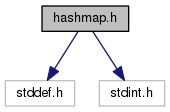
\includegraphics[width=200pt]{hashmap_8h__incl}
\end{center}
\end{figure}
This graph shows which files directly or indirectly include this file\+:
\nopagebreak
\begin{figure}[H]
\begin{center}
\leavevmode
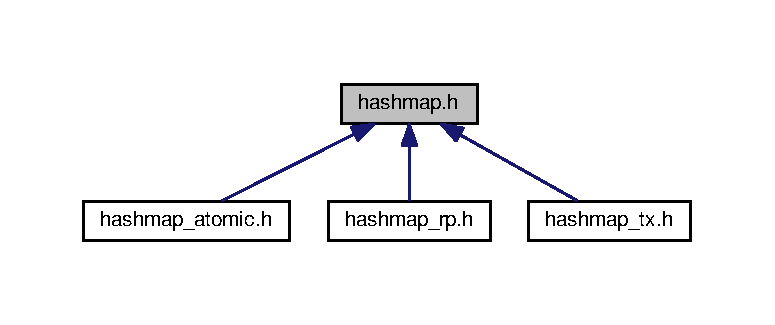
\includegraphics[width=350pt]{hashmap_8h__dep__incl}
\end{center}
\end{figure}
\subsection*{Classes}
\begin{DoxyCompactItemize}
\item 
struct \hyperlink{structhashmap__args}{hashmap\+\_\+args}
\end{DoxyCompactItemize}
\subsection*{Enumerations}
\begin{DoxyCompactItemize}
\item 
enum {\bfseries hashmap\+\_\+cmd} \{ {\bfseries H\+A\+S\+H\+M\+A\+P\+\_\+\+C\+M\+D\+\_\+\+R\+E\+B\+U\+I\+LD}, 
{\bfseries H\+A\+S\+H\+M\+A\+P\+\_\+\+C\+M\+D\+\_\+\+D\+E\+B\+UG}
 \}\hypertarget{hashmap_8h_a06616991d22cc27ebd6f17d026241386}{}\label{hashmap_8h_a06616991d22cc27ebd6f17d026241386}

\end{DoxyCompactItemize}


\subsection{Detailed Description}
Hashmap implementation in persistent memory. 

Details. 
\hypertarget{hashmap__atomic_8h}{}\section{hashmap/hashmap\+\_\+atomic.h File Reference}
\label{hashmap__atomic_8h}\index{hashmap/hashmap\+\_\+atomic.\+h@{hashmap/hashmap\+\_\+atomic.\+h}}


Implementation of atomic hashmap, where inserts are coordinated to be one after the other.  


{\ttfamily \#include $<$stddef.\+h$>$}\newline
{\ttfamily \#include $<$stdint.\+h$>$}\newline
{\ttfamily \#include $<$hashmap.\+h$>$}\newline
{\ttfamily \#include $<$libpmemobj.\+h$>$}\newline
Include dependency graph for hashmap\+\_\+atomic.\+h\+:
% FIG 0
\subsection*{Macros}
\begin{DoxyCompactItemize}
\item 
\mbox{\Hypertarget{hashmap__atomic_8h_ac7a2806ad6610fce7f1a06b8777c773f}\label{hashmap__atomic_8h_ac7a2806ad6610fce7f1a06b8777c773f}} 
\#define {\bfseries H\+A\+S\+H\+M\+A\+P\+\_\+\+A\+T\+O\+M\+I\+C\+\_\+\+T\+Y\+P\+E\+\_\+\+O\+F\+F\+S\+ET}~1000
\end{DoxyCompactItemize}
\subsection*{Functions}
\begin{DoxyCompactItemize}
\item 
\mbox{\Hypertarget{hashmap__atomic_8h_a10298cea42cfb536c27f9c6a4abeecc1}\label{hashmap__atomic_8h_a10298cea42cfb536c27f9c6a4abeecc1}} 
{\bfseries T\+O\+I\+D\+\_\+\+D\+E\+C\+L\+A\+RE} (struct \hyperlink{structhashmap__atomic}{hashmap\+\_\+atomic}, H\+A\+S\+H\+M\+A\+P\+\_\+\+A\+T\+O\+M\+I\+C\+\_\+\+T\+Y\+P\+E\+\_\+\+O\+F\+F\+S\+ET+0)
\item 
\mbox{\Hypertarget{hashmap__atomic_8h_a598708b91dce5756734872ba7591f275}\label{hashmap__atomic_8h_a598708b91dce5756734872ba7591f275}} 
int {\bfseries hm\+\_\+atomic\+\_\+check} (P\+M\+E\+Mobjpool $\ast$pop, T\+O\+ID(struct \hyperlink{structhashmap__atomic}{hashmap\+\_\+atomic}) hashmap)
\item 
\mbox{\Hypertarget{hashmap__atomic_8h_acbb4c401a679ca192b8758cde9befce8}\label{hashmap__atomic_8h_acbb4c401a679ca192b8758cde9befce8}} 
int {\bfseries hm\+\_\+atomic\+\_\+create} (P\+M\+E\+Mobjpool $\ast$pop, T\+O\+ID(struct \hyperlink{structhashmap__atomic}{hashmap\+\_\+atomic}) $\ast$map, void $\ast$arg)
\item 
\mbox{\Hypertarget{hashmap__atomic_8h_a04f0c019c9846769951407ba5a03fb16}\label{hashmap__atomic_8h_a04f0c019c9846769951407ba5a03fb16}} 
int {\bfseries hm\+\_\+atomic\+\_\+init} (P\+M\+E\+Mobjpool $\ast$pop, T\+O\+ID(struct \hyperlink{structhashmap__atomic}{hashmap\+\_\+atomic}) hashmap)
\item 
\mbox{\Hypertarget{hashmap__atomic_8h_af9e2aa6113e1ce3b5dbaac973ebda554}\label{hashmap__atomic_8h_af9e2aa6113e1ce3b5dbaac973ebda554}} 
int {\bfseries hm\+\_\+atomic\+\_\+insert} (P\+M\+E\+Mobjpool $\ast$pop, T\+O\+ID(struct \hyperlink{structhashmap__atomic}{hashmap\+\_\+atomic}) hashmap, uint64\+\_\+t key, \hyperlink{structpmemoid}{P\+M\+E\+Moid} value)
\item 
\mbox{\Hypertarget{hashmap__atomic_8h_a271644b8a80804a39314ce6cf7582b33}\label{hashmap__atomic_8h_a271644b8a80804a39314ce6cf7582b33}} 
\hyperlink{structpmemoid}{P\+M\+E\+Moid} {\bfseries hm\+\_\+atomic\+\_\+remove} (P\+M\+E\+Mobjpool $\ast$pop, T\+O\+ID(struct \hyperlink{structhashmap__atomic}{hashmap\+\_\+atomic}) hashmap, uint64\+\_\+t key)
\item 
\mbox{\Hypertarget{hashmap__atomic_8h_ad203219cd5cd5a4d69661004b53f193f}\label{hashmap__atomic_8h_ad203219cd5cd5a4d69661004b53f193f}} 
\hyperlink{structpmemoid}{P\+M\+E\+Moid} {\bfseries hm\+\_\+atomic\+\_\+get} (P\+M\+E\+Mobjpool $\ast$pop, T\+O\+ID(struct \hyperlink{structhashmap__atomic}{hashmap\+\_\+atomic}) hashmap, uint64\+\_\+t key)
\item 
\mbox{\Hypertarget{hashmap__atomic_8h_aaf062e36e2b6e22bc832847d5ee67dd1}\label{hashmap__atomic_8h_aaf062e36e2b6e22bc832847d5ee67dd1}} 
int {\bfseries hm\+\_\+atomic\+\_\+lookup} (P\+M\+E\+Mobjpool $\ast$pop, T\+O\+ID(struct \hyperlink{structhashmap__atomic}{hashmap\+\_\+atomic}) hashmap, uint64\+\_\+t key)
\item 
\mbox{\Hypertarget{hashmap__atomic_8h_af1a055b49bce902e78ef3774e6ea5918}\label{hashmap__atomic_8h_af1a055b49bce902e78ef3774e6ea5918}} 
int {\bfseries hm\+\_\+atomic\+\_\+foreach} (P\+M\+E\+Mobjpool $\ast$pop, T\+O\+ID(struct \hyperlink{structhashmap__atomic}{hashmap\+\_\+atomic}) hashmap, int($\ast$cb)(uint64\+\_\+t key, \hyperlink{structpmemoid}{P\+M\+E\+Moid} value, void $\ast$arg), void $\ast$arg)
\item 
\mbox{\Hypertarget{hashmap__atomic_8h_a6cb2f755fcf3b9b7c0361754ce6444ce}\label{hashmap__atomic_8h_a6cb2f755fcf3b9b7c0361754ce6444ce}} 
size\+\_\+t {\bfseries hm\+\_\+atomic\+\_\+count} (P\+M\+E\+Mobjpool $\ast$pop, T\+O\+ID(struct \hyperlink{structhashmap__atomic}{hashmap\+\_\+atomic}) hashmap)
\item 
\mbox{\Hypertarget{hashmap__atomic_8h_a1b44897be6a25691a516e1af2d2a2e26}\label{hashmap__atomic_8h_a1b44897be6a25691a516e1af2d2a2e26}} 
int {\bfseries hm\+\_\+atomic\+\_\+cmd} (P\+M\+E\+Mobjpool $\ast$pop, T\+O\+ID(struct \hyperlink{structhashmap__atomic}{hashmap\+\_\+atomic}) hashmap, unsigned cmd, uint64\+\_\+t arg)
\end{DoxyCompactItemize}


\subsection{Detailed Description}
Implementation of atomic hashmap, where inserts are coordinated to be one after the other. 

Details. 
\hypertarget{fifo_8c}{}\section{linkedlist/fifo.c File Reference}
\label{fifo_8c}\index{linkedlist/fifo.\+c@{linkedlist/fifo.\+c}}


Example of a tail queue usage.  


{\ttfamily \#include $<$ex\+\_\+common.\+h$>$}\newline
{\ttfamily \#include $<$stdio.\+h$>$}\newline
{\ttfamily \#include $<$stdlib.\+h$>$}\newline
{\ttfamily \#include $<$string.\+h$>$}\newline
{\ttfamily \#include \char`\"{}pmemobj\+\_\+list.\+h\char`\"{}}\newline
Include dependency graph for fifo.\+c\+:
% FIG 0
\subsection*{Classes}
\begin{DoxyCompactItemize}
\item 
struct \hyperlink{structfifo__root}{fifo\+\_\+root}
\item 
struct \hyperlink{structtqnode}{tqnode}
\end{DoxyCompactItemize}
\subsection*{Functions}
\begin{DoxyCompactItemize}
\item 
\mbox{\Hypertarget{fifo_8c_abdfca56bbdeb6ee593a723f9d78f9a62}\label{fifo_8c_abdfca56bbdeb6ee593a723f9d78f9a62}} 
{\bfseries P\+O\+B\+J\+\_\+\+L\+A\+Y\+O\+U\+T\+\_\+\+B\+E\+G\+IN} (list)
\item 
\mbox{\Hypertarget{fifo_8c_a72a69504e27903923162e68f33492559}\label{fifo_8c_a72a69504e27903923162e68f33492559}} 
{\bfseries P\+O\+B\+J\+\_\+\+L\+A\+Y\+O\+U\+T\+\_\+\+R\+O\+OT} (list, struct \hyperlink{structfifo__root}{fifo\+\_\+root})
\item 
\mbox{\Hypertarget{fifo_8c_ab252059e1bccb1a99700bface1eed039}\label{fifo_8c_ab252059e1bccb1a99700bface1eed039}} 
{\bfseries P\+O\+B\+J\+\_\+\+L\+A\+Y\+O\+U\+T\+\_\+\+T\+O\+ID} (list, struct \hyperlink{structtqnode}{tqnode})
\item 
\mbox{\Hypertarget{fifo_8c_ac781e28175878fee2882fdec9fe0e5ff}\label{fifo_8c_ac781e28175878fee2882fdec9fe0e5ff}} 
{\bfseries P\+O\+B\+J\+\_\+\+L\+A\+Y\+O\+U\+T\+\_\+\+E\+ND} (list)
\item 
\mbox{\Hypertarget{fifo_8c_a09f61fb0bd8623654811d0cfdd6b6715}\label{fifo_8c_a09f61fb0bd8623654811d0cfdd6b6715}} 
{\bfseries P\+O\+B\+J\+\_\+\+T\+A\+I\+L\+Q\+\_\+\+H\+E\+AD} (tqueuehead, struct \hyperlink{structtqnode}{tqnode})
\item 
int \hyperlink{fifo_8c_ac0f2228420376f4db7e1274f2b41667c}{main} (int argc, const char $\ast$argv\mbox{[}$\,$\mbox{]})
\end{DoxyCompactItemize}


\subsection{Detailed Description}
Example of a tail queue usage. 

Details. 

\subsection{Function Documentation}
\mbox{\Hypertarget{fifo_8c_ac0f2228420376f4db7e1274f2b41667c}\label{fifo_8c_ac0f2228420376f4db7e1274f2b41667c}} 
\index{fifo.\+c@{fifo.\+c}!main@{main}}
\index{main@{main}!fifo.\+c@{fifo.\+c}}
\subsubsection{\texorpdfstring{main()}{main()}}
{\footnotesize\ttfamily int main (\begin{DoxyParamCaption}\item[{int}]{argc,  }\item[{const char $\ast$}]{argv\mbox{[}$\,$\mbox{]} }\end{DoxyParamCaption})}

Initially we create a pmempool, and we initialize a path. The arguments here, represent the following variables which are inputted. The first argument is the path. The second argument is the operation , indicating whether it is an insert, remove or print. This is coherent with the way a queue regularly works, with it having remove and print the first element in the queue. And then insert to the end of the queue. This one is an indication of the same.

$<$ Detailed description after the member

Checking if insert occurs, and proceeding accordingly by doing a pmemobj insert head. Here we take the third argument, which is the data.
\hypertarget{pmemobj__list_8h}{}\section{linkedlist/pmemobj\+\_\+list.h File Reference}
\label{pmemobj__list_8h}\index{linkedlist/pmemobj\+\_\+list.\+h@{linkedlist/pmemobj\+\_\+list.\+h}}


Pmemobj implementations for pointer manipulation in persistent memory. These are accessed by the fifo queue operations.  


{\ttfamily \#include $<$libpmemobj.\+h$>$}\newline
Include dependency graph for pmemobj\+\_\+list.\+h\+:
% FIG 0
This graph shows which files directly or indirectly include this file\+:
% FIG 1
\subsection*{Macros}
\begin{DoxyCompactItemize}
\item 
\#define {\bfseries P\+O\+B\+J\+\_\+\+S\+L\+I\+S\+T\+\_\+\+H\+E\+AD}(name,  type)
\item 
\#define {\bfseries P\+O\+B\+J\+\_\+\+S\+L\+I\+S\+T\+\_\+\+E\+N\+T\+RY}(type)
\item 
\mbox{\Hypertarget{pmemobj__list_8h_a82c18e0b0cf89215188929dc94b796cc}\label{pmemobj__list_8h_a82c18e0b0cf89215188929dc94b796cc}} 
\#define {\bfseries P\+O\+B\+J\+\_\+\+S\+L\+I\+S\+T\+\_\+\+E\+M\+P\+TY}(head)~(T\+O\+I\+D\+\_\+\+I\+S\+\_\+\+N\+U\+LL((head)-\/$>$pe\+\_\+first))
\item 
\mbox{\Hypertarget{pmemobj__list_8h_a06a4bba6ee48cd2466fe1d6aa0fc2760}\label{pmemobj__list_8h_a06a4bba6ee48cd2466fe1d6aa0fc2760}} 
\#define {\bfseries P\+O\+B\+J\+\_\+\+S\+L\+I\+S\+T\+\_\+\+F\+I\+R\+ST}(head)~((head)-\/$>$pe\+\_\+first)
\item 
\mbox{\Hypertarget{pmemobj__list_8h_a7bb1e476d45fe6d569d55f5a55d9542d}\label{pmemobj__list_8h_a7bb1e476d45fe6d569d55f5a55d9542d}} 
\#define {\bfseries P\+O\+B\+J\+\_\+\+S\+L\+I\+S\+T\+\_\+\+N\+E\+XT}(elm,  field)~(D\+\_\+\+RO(elm)-\/$>$field.\+pe\+\_\+next)
\item 
\#define {\bfseries P\+O\+B\+J\+\_\+\+S\+L\+I\+S\+T\+\_\+\+I\+N\+IT}(head)
\item 
\#define {\bfseries P\+O\+B\+J\+\_\+\+S\+L\+I\+S\+T\+\_\+\+I\+N\+S\+E\+R\+T\+\_\+\+H\+E\+AD}(head,  elm,  field)
\item 
\#define {\bfseries P\+O\+B\+J\+\_\+\+S\+L\+I\+S\+T\+\_\+\+I\+N\+S\+E\+R\+T\+\_\+\+A\+F\+T\+ER}(slistelm,  elm,  field)
\item 
\#define {\bfseries P\+O\+B\+J\+\_\+\+S\+L\+I\+S\+T\+\_\+\+R\+E\+M\+O\+V\+E\+\_\+\+H\+E\+AD}(head,  field)
\item 
\#define {\bfseries P\+O\+B\+J\+\_\+\+S\+L\+I\+S\+T\+\_\+\+R\+E\+M\+O\+VE}(head,  elm,  field)
\item 
\#define {\bfseries P\+O\+B\+J\+\_\+\+S\+L\+I\+S\+T\+\_\+\+R\+E\+M\+O\+V\+E\+\_\+\+F\+R\+EE}(head,  elm,  field)
\item 
\#define {\bfseries P\+O\+B\+J\+\_\+\+S\+L\+I\+S\+T\+\_\+\+F\+O\+R\+E\+A\+CH}(var,  head,  field)
\item 
\#define {\bfseries P\+O\+B\+J\+\_\+\+T\+A\+I\+L\+Q\+\_\+\+E\+N\+T\+RY}(type)
\item 
\#define {\bfseries P\+O\+B\+J\+\_\+\+T\+A\+I\+L\+Q\+\_\+\+H\+E\+AD}(name,  type)
\item 
\#define \hyperlink{pmemobj__list_8h_a4039b5980a3a61a32281620c19238703}{P\+O\+B\+J\+\_\+\+T\+A\+I\+L\+Q\+\_\+\+F\+I\+R\+ST}(head)~((head)-\/$>$pe\+\_\+first)
\item 
\#define \hyperlink{pmemobj__list_8h_ab1a1ab59d094a22fd65d12e7d4768550}{P\+O\+B\+J\+\_\+\+T\+A\+I\+L\+Q\+\_\+\+L\+A\+ST}(head)~((head)-\/$>$pe\+\_\+last)
\item 
\mbox{\Hypertarget{pmemobj__list_8h_af7a0a3245e9955875d2252e6bf27cc5e}\label{pmemobj__list_8h_af7a0a3245e9955875d2252e6bf27cc5e}} 
\#define {\bfseries P\+O\+B\+J\+\_\+\+T\+A\+I\+L\+Q\+\_\+\+E\+M\+P\+TY}(head)~(T\+O\+I\+D\+\_\+\+I\+S\+\_\+\+N\+U\+LL((head)-\/$>$pe\+\_\+first))
\item 
\mbox{\Hypertarget{pmemobj__list_8h_a09ac1601472384f0c6a04633d7ef375e}\label{pmemobj__list_8h_a09ac1601472384f0c6a04633d7ef375e}} 
\#define {\bfseries P\+O\+B\+J\+\_\+\+T\+A\+I\+L\+Q\+\_\+\+N\+E\+XT}(elm,  field)~(D\+\_\+\+RO(elm)-\/$>$field.\+pe\+\_\+next)
\item 
\mbox{\Hypertarget{pmemobj__list_8h_ad8382c7ac332292ef18a30c98ad5683a}\label{pmemobj__list_8h_ad8382c7ac332292ef18a30c98ad5683a}} 
\#define {\bfseries P\+O\+B\+J\+\_\+\+T\+A\+I\+L\+Q\+\_\+\+P\+R\+EV}(elm,  field)~(D\+\_\+\+RO(elm)-\/$>$field.\+pe\+\_\+prev)
\item 
\#define {\bfseries \+\_\+\+P\+O\+B\+J\+\_\+\+S\+W\+A\+P\+\_\+\+P\+TR}(elm,  field)
\item 
\#define {\bfseries P\+O\+B\+J\+\_\+\+T\+A\+I\+L\+Q\+\_\+\+S\+W\+A\+P\+\_\+\+H\+E\+A\+D\+\_\+\+T\+A\+IL}(head,  field)
\item 
\#define {\bfseries P\+O\+B\+J\+\_\+\+T\+A\+I\+L\+Q\+\_\+\+F\+O\+R\+E\+A\+CH}(var,  head,  field)
\item 
\#define {\bfseries P\+O\+B\+J\+\_\+\+T\+A\+I\+L\+Q\+\_\+\+F\+O\+R\+E\+A\+C\+H\+\_\+\+R\+E\+V\+E\+R\+SE}(var,  head,  field)
\item 
\#define \hyperlink{pmemobj__list_8h_a74f5d9cb3d2048db986dd0677bee5a12}{P\+O\+B\+J\+\_\+\+T\+A\+I\+L\+Q\+\_\+\+I\+N\+IT}(head)
\item 
\#define \hyperlink{pmemobj__list_8h_ae64ca8f8f0408a5cbad62d13d20d6c34}{P\+O\+B\+J\+\_\+\+T\+A\+I\+L\+Q\+\_\+\+I\+N\+S\+E\+R\+T\+\_\+\+H\+E\+AD}(head,  elm,  field)
\item 
\#define {\bfseries P\+O\+B\+J\+\_\+\+T\+A\+I\+L\+Q\+\_\+\+I\+N\+S\+E\+R\+T\+\_\+\+T\+A\+IL}(head,  elm,  field)
\item 
\#define {\bfseries P\+O\+B\+J\+\_\+\+T\+A\+I\+L\+Q\+\_\+\+I\+N\+S\+E\+R\+T\+\_\+\+A\+F\+T\+ER}(listelm,  elm,  field)
\item 
\#define {\bfseries P\+O\+B\+J\+\_\+\+T\+A\+I\+L\+Q\+\_\+\+I\+N\+S\+E\+R\+T\+\_\+\+B\+E\+F\+O\+RE}(listelm,  elm,  field)
\item 
\#define {\bfseries P\+O\+B\+J\+\_\+\+T\+A\+I\+L\+Q\+\_\+\+R\+E\+M\+O\+VE}(head,  elm,  field)
\item 
\#define {\bfseries P\+O\+B\+J\+\_\+\+T\+A\+I\+L\+Q\+\_\+\+R\+E\+M\+O\+V\+E\+\_\+\+F\+R\+EE}(head,  elm,  field)
\item 
\#define {\bfseries P\+O\+B\+J\+\_\+\+T\+A\+I\+L\+Q\+\_\+\+M\+O\+V\+E\+\_\+\+E\+L\+E\+M\+E\+N\+T\+\_\+\+H\+E\+AD}(head,  elm,  field)
\item 
\#define {\bfseries P\+O\+B\+J\+\_\+\+T\+A\+I\+L\+Q\+\_\+\+M\+O\+V\+E\+\_\+\+E\+L\+E\+M\+E\+N\+T\+\_\+\+T\+A\+IL}(head,  elm,  field)
\end{DoxyCompactItemize}


\subsection{Detailed Description}
Pmemobj implementations for pointer manipulation in persistent memory. These are accessed by the fifo queue operations. 

Details. 

\subsection{Macro Definition Documentation}
\mbox{\Hypertarget{pmemobj__list_8h_a501a7da17b4b12104cec60fc6601cd4a}\label{pmemobj__list_8h_a501a7da17b4b12104cec60fc6601cd4a}} 
\index{pmemobj\+\_\+list.\+h@{pmemobj\+\_\+list.\+h}!\+\_\+\+P\+O\+B\+J\+\_\+\+S\+W\+A\+P\+\_\+\+P\+TR@{\+\_\+\+P\+O\+B\+J\+\_\+\+S\+W\+A\+P\+\_\+\+P\+TR}}
\index{\+\_\+\+P\+O\+B\+J\+\_\+\+S\+W\+A\+P\+\_\+\+P\+TR@{\+\_\+\+P\+O\+B\+J\+\_\+\+S\+W\+A\+P\+\_\+\+P\+TR}!pmemobj\+\_\+list.\+h@{pmemobj\+\_\+list.\+h}}
\subsubsection{\texorpdfstring{\+\_\+\+P\+O\+B\+J\+\_\+\+S\+W\+A\+P\+\_\+\+P\+TR}{\_POBJ\_SWAP\_PTR}}
{\footnotesize\ttfamily \#define \+\_\+\+P\+O\+B\+J\+\_\+\+S\+W\+A\+P\+\_\+\+P\+TR(\begin{DoxyParamCaption}\item[{}]{elm,  }\item[{}]{field }\end{DoxyParamCaption})}

{\bfseries Value\+:}
\begin{DoxyCode}
\textcolor{keywordflow}{do} \{\(\backslash\)
    TOID\_TYPEOF(elm) *elm\_ptr = D\_RW(elm);\(\backslash\)
    TX\_ADD\_DIRECT(&elm\_ptr->field);\(\backslash\)
    \_\_typeof\_\_(elm) temp = elm\_ptr->field.pe\_prev;\(\backslash\)
    elm\_ptr->field.pe\_prev = elm\_ptr->field.pe\_next;\(\backslash\)
    elm\_ptr->field.pe\_next = temp;\(\backslash\)
\} \textcolor{keywordflow}{while} (0)
\end{DoxyCode}
\mbox{\Hypertarget{pmemobj__list_8h_a8ccdb6deffb78cd637bb38ef1b95ce00}\label{pmemobj__list_8h_a8ccdb6deffb78cd637bb38ef1b95ce00}} 
\index{pmemobj\+\_\+list.\+h@{pmemobj\+\_\+list.\+h}!P\+O\+B\+J\+\_\+\+S\+L\+I\+S\+T\+\_\+\+E\+N\+T\+RY@{P\+O\+B\+J\+\_\+\+S\+L\+I\+S\+T\+\_\+\+E\+N\+T\+RY}}
\index{P\+O\+B\+J\+\_\+\+S\+L\+I\+S\+T\+\_\+\+E\+N\+T\+RY@{P\+O\+B\+J\+\_\+\+S\+L\+I\+S\+T\+\_\+\+E\+N\+T\+RY}!pmemobj\+\_\+list.\+h@{pmemobj\+\_\+list.\+h}}
\subsubsection{\texorpdfstring{P\+O\+B\+J\+\_\+\+S\+L\+I\+S\+T\+\_\+\+E\+N\+T\+RY}{POBJ\_SLIST\_ENTRY}}
{\footnotesize\ttfamily \#define P\+O\+B\+J\+\_\+\+S\+L\+I\+S\+T\+\_\+\+E\+N\+T\+RY(\begin{DoxyParamCaption}\item[{}]{type }\end{DoxyParamCaption})}

{\bfseries Value\+:}
\begin{DoxyCode}
\textcolor{keyword}{struct }\{\(\backslash\)
    TOID(type) pe\_next;\(\backslash\)
\}
\end{DoxyCode}
\mbox{\Hypertarget{pmemobj__list_8h_a75e0d8c5f41972d1e93b0d78de79407e}\label{pmemobj__list_8h_a75e0d8c5f41972d1e93b0d78de79407e}} 
\index{pmemobj\+\_\+list.\+h@{pmemobj\+\_\+list.\+h}!P\+O\+B\+J\+\_\+\+S\+L\+I\+S\+T\+\_\+\+F\+O\+R\+E\+A\+CH@{P\+O\+B\+J\+\_\+\+S\+L\+I\+S\+T\+\_\+\+F\+O\+R\+E\+A\+CH}}
\index{P\+O\+B\+J\+\_\+\+S\+L\+I\+S\+T\+\_\+\+F\+O\+R\+E\+A\+CH@{P\+O\+B\+J\+\_\+\+S\+L\+I\+S\+T\+\_\+\+F\+O\+R\+E\+A\+CH}!pmemobj\+\_\+list.\+h@{pmemobj\+\_\+list.\+h}}
\subsubsection{\texorpdfstring{P\+O\+B\+J\+\_\+\+S\+L\+I\+S\+T\+\_\+\+F\+O\+R\+E\+A\+CH}{POBJ\_SLIST\_FOREACH}}
{\footnotesize\ttfamily \#define P\+O\+B\+J\+\_\+\+S\+L\+I\+S\+T\+\_\+\+F\+O\+R\+E\+A\+CH(\begin{DoxyParamCaption}\item[{}]{var,  }\item[{}]{head,  }\item[{}]{field }\end{DoxyParamCaption})}

{\bfseries Value\+:}
\begin{DoxyCode}
\textcolor{keywordflow}{for} ((var) = POBJ\_SLIST\_FIRST(head);\(\backslash\)
        !TOID\_IS\_NULL(var);\(\backslash\)
        var = POBJ\_SLIST\_NEXT(var, field))
\end{DoxyCode}
\mbox{\Hypertarget{pmemobj__list_8h_a020d23d0bf1f4831bea29d9741475f2c}\label{pmemobj__list_8h_a020d23d0bf1f4831bea29d9741475f2c}} 
\index{pmemobj\+\_\+list.\+h@{pmemobj\+\_\+list.\+h}!P\+O\+B\+J\+\_\+\+S\+L\+I\+S\+T\+\_\+\+H\+E\+AD@{P\+O\+B\+J\+\_\+\+S\+L\+I\+S\+T\+\_\+\+H\+E\+AD}}
\index{P\+O\+B\+J\+\_\+\+S\+L\+I\+S\+T\+\_\+\+H\+E\+AD@{P\+O\+B\+J\+\_\+\+S\+L\+I\+S\+T\+\_\+\+H\+E\+AD}!pmemobj\+\_\+list.\+h@{pmemobj\+\_\+list.\+h}}
\subsubsection{\texorpdfstring{P\+O\+B\+J\+\_\+\+S\+L\+I\+S\+T\+\_\+\+H\+E\+AD}{POBJ\_SLIST\_HEAD}}
{\footnotesize\ttfamily \#define P\+O\+B\+J\+\_\+\+S\+L\+I\+S\+T\+\_\+\+H\+E\+AD(\begin{DoxyParamCaption}\item[{}]{name,  }\item[{}]{type }\end{DoxyParamCaption})}

{\bfseries Value\+:}
\begin{DoxyCode}
\textcolor{keyword}{struct }name \{\(\backslash\)
    TOID(type) pe\_first;\(\backslash\)
\}
\end{DoxyCode}
\mbox{\Hypertarget{pmemobj__list_8h_a91b31c2a97d1bc4cbd376438958b7253}\label{pmemobj__list_8h_a91b31c2a97d1bc4cbd376438958b7253}} 
\index{pmemobj\+\_\+list.\+h@{pmemobj\+\_\+list.\+h}!P\+O\+B\+J\+\_\+\+S\+L\+I\+S\+T\+\_\+\+I\+N\+IT@{P\+O\+B\+J\+\_\+\+S\+L\+I\+S\+T\+\_\+\+I\+N\+IT}}
\index{P\+O\+B\+J\+\_\+\+S\+L\+I\+S\+T\+\_\+\+I\+N\+IT@{P\+O\+B\+J\+\_\+\+S\+L\+I\+S\+T\+\_\+\+I\+N\+IT}!pmemobj\+\_\+list.\+h@{pmemobj\+\_\+list.\+h}}
\subsubsection{\texorpdfstring{P\+O\+B\+J\+\_\+\+S\+L\+I\+S\+T\+\_\+\+I\+N\+IT}{POBJ\_SLIST\_INIT}}
{\footnotesize\ttfamily \#define P\+O\+B\+J\+\_\+\+S\+L\+I\+S\+T\+\_\+\+I\+N\+IT(\begin{DoxyParamCaption}\item[{}]{head }\end{DoxyParamCaption})}

{\bfseries Value\+:}
\begin{DoxyCode}
\textcolor{keywordflow}{do} \{\(\backslash\)
    TX\_ADD\_DIRECT(&(head)->pe\_first);\(\backslash\)
    TOID\_ASSIGN((head)->pe\_first, OID\_NULL);\(\backslash\)
\} \textcolor{keywordflow}{while} (0)
\end{DoxyCode}
\mbox{\Hypertarget{pmemobj__list_8h_a9c8f39cc1858248c5f39c218b2b16ead}\label{pmemobj__list_8h_a9c8f39cc1858248c5f39c218b2b16ead}} 
\index{pmemobj\+\_\+list.\+h@{pmemobj\+\_\+list.\+h}!P\+O\+B\+J\+\_\+\+S\+L\+I\+S\+T\+\_\+\+I\+N\+S\+E\+R\+T\+\_\+\+A\+F\+T\+ER@{P\+O\+B\+J\+\_\+\+S\+L\+I\+S\+T\+\_\+\+I\+N\+S\+E\+R\+T\+\_\+\+A\+F\+T\+ER}}
\index{P\+O\+B\+J\+\_\+\+S\+L\+I\+S\+T\+\_\+\+I\+N\+S\+E\+R\+T\+\_\+\+A\+F\+T\+ER@{P\+O\+B\+J\+\_\+\+S\+L\+I\+S\+T\+\_\+\+I\+N\+S\+E\+R\+T\+\_\+\+A\+F\+T\+ER}!pmemobj\+\_\+list.\+h@{pmemobj\+\_\+list.\+h}}
\subsubsection{\texorpdfstring{P\+O\+B\+J\+\_\+\+S\+L\+I\+S\+T\+\_\+\+I\+N\+S\+E\+R\+T\+\_\+\+A\+F\+T\+ER}{POBJ\_SLIST\_INSERT\_AFTER}}
{\footnotesize\ttfamily \#define P\+O\+B\+J\+\_\+\+S\+L\+I\+S\+T\+\_\+\+I\+N\+S\+E\+R\+T\+\_\+\+A\+F\+T\+ER(\begin{DoxyParamCaption}\item[{}]{slistelm,  }\item[{}]{elm,  }\item[{}]{field }\end{DoxyParamCaption})}

{\bfseries Value\+:}
\begin{DoxyCode}
\textcolor{keywordflow}{do} \{\(\backslash\)
    TOID\_TYPEOF(slistelm) *slistelm\_ptr = D\_RW(slistelm);\(\backslash\)
    TOID\_TYPEOF(elm) *elm\_ptr = D\_RW(elm);\(\backslash\)
    TX\_ADD\_DIRECT(&elm\_ptr->field.pe\_next);\(\backslash\)
    elm\_ptr->field.pe\_next = slistelm\_ptr->field.pe\_next;\(\backslash\)
    TX\_ADD\_DIRECT(&slistelm\_ptr->field.pe\_next);\(\backslash\)
    slistelm\_ptr->field.pe\_next = elm;\(\backslash\)
\} \textcolor{keywordflow}{while} (0)
\end{DoxyCode}
\mbox{\Hypertarget{pmemobj__list_8h_ae5b43f35c6a97975daf1e480b87af7f1}\label{pmemobj__list_8h_ae5b43f35c6a97975daf1e480b87af7f1}} 
\index{pmemobj\+\_\+list.\+h@{pmemobj\+\_\+list.\+h}!P\+O\+B\+J\+\_\+\+S\+L\+I\+S\+T\+\_\+\+I\+N\+S\+E\+R\+T\+\_\+\+H\+E\+AD@{P\+O\+B\+J\+\_\+\+S\+L\+I\+S\+T\+\_\+\+I\+N\+S\+E\+R\+T\+\_\+\+H\+E\+AD}}
\index{P\+O\+B\+J\+\_\+\+S\+L\+I\+S\+T\+\_\+\+I\+N\+S\+E\+R\+T\+\_\+\+H\+E\+AD@{P\+O\+B\+J\+\_\+\+S\+L\+I\+S\+T\+\_\+\+I\+N\+S\+E\+R\+T\+\_\+\+H\+E\+AD}!pmemobj\+\_\+list.\+h@{pmemobj\+\_\+list.\+h}}
\subsubsection{\texorpdfstring{P\+O\+B\+J\+\_\+\+S\+L\+I\+S\+T\+\_\+\+I\+N\+S\+E\+R\+T\+\_\+\+H\+E\+AD}{POBJ\_SLIST\_INSERT\_HEAD}}
{\footnotesize\ttfamily \#define P\+O\+B\+J\+\_\+\+S\+L\+I\+S\+T\+\_\+\+I\+N\+S\+E\+R\+T\+\_\+\+H\+E\+AD(\begin{DoxyParamCaption}\item[{}]{head,  }\item[{}]{elm,  }\item[{}]{field }\end{DoxyParamCaption})}

{\bfseries Value\+:}
\begin{DoxyCode}
\textcolor{keywordflow}{do} \{\(\backslash\)
    TOID\_TYPEOF(elm) *elm\_ptr = D\_RW(elm);\(\backslash\)
    TX\_ADD\_DIRECT(&elm\_ptr->field.pe\_next);\(\backslash\)
    elm\_ptr->field.pe\_next = (head)->pe\_first;\(\backslash\)
    TX\_SET\_DIRECT(head, pe\_first, elm);\(\backslash\)
\} \textcolor{keywordflow}{while} (0)
\end{DoxyCode}
\mbox{\Hypertarget{pmemobj__list_8h_a1b823b3d55390af28b67a08e84f91046}\label{pmemobj__list_8h_a1b823b3d55390af28b67a08e84f91046}} 
\index{pmemobj\+\_\+list.\+h@{pmemobj\+\_\+list.\+h}!P\+O\+B\+J\+\_\+\+S\+L\+I\+S\+T\+\_\+\+R\+E\+M\+O\+VE@{P\+O\+B\+J\+\_\+\+S\+L\+I\+S\+T\+\_\+\+R\+E\+M\+O\+VE}}
\index{P\+O\+B\+J\+\_\+\+S\+L\+I\+S\+T\+\_\+\+R\+E\+M\+O\+VE@{P\+O\+B\+J\+\_\+\+S\+L\+I\+S\+T\+\_\+\+R\+E\+M\+O\+VE}!pmemobj\+\_\+list.\+h@{pmemobj\+\_\+list.\+h}}
\subsubsection{\texorpdfstring{P\+O\+B\+J\+\_\+\+S\+L\+I\+S\+T\+\_\+\+R\+E\+M\+O\+VE}{POBJ\_SLIST\_REMOVE}}
{\footnotesize\ttfamily \#define P\+O\+B\+J\+\_\+\+S\+L\+I\+S\+T\+\_\+\+R\+E\+M\+O\+VE(\begin{DoxyParamCaption}\item[{}]{head,  }\item[{}]{elm,  }\item[{}]{field }\end{DoxyParamCaption})}

{\bfseries Value\+:}
\begin{DoxyCode}
\textcolor{keywordflow}{do} \{\(\backslash\)
    if (TOID\_EQUALS((head)->pe\_first, elm)) \{\(\backslash\)
        POBJ\_SLIST\_REMOVE\_HEAD(head, field);\(\backslash\)
    \} \textcolor{keywordflow}{else} \{\(\backslash\)
        TOID\_TYPEOF(elm) *curelm\_ptr = D\_RW((head)->pe\_first);\(\backslash\)
        while (!TOID\_EQUALS(curelm\_ptr->field.pe\_next, elm))\(\backslash\)
            curelm\_ptr = D\_RW(curelm\_ptr->field.pe\_next);\(\backslash\)
        TX\_ADD\_DIRECT(&curelm\_ptr->field.pe\_next);\(\backslash\)
        curelm\_ptr->field.pe\_next = D\_RO(elm)->field.pe\_next;\(\backslash\)
    \}\(\backslash\)
\} \textcolor{keywordflow}{while} (0)
\end{DoxyCode}
\mbox{\Hypertarget{pmemobj__list_8h_a893c3b265d8a7ff6f8c2ae5d24fdea5e}\label{pmemobj__list_8h_a893c3b265d8a7ff6f8c2ae5d24fdea5e}} 
\index{pmemobj\+\_\+list.\+h@{pmemobj\+\_\+list.\+h}!P\+O\+B\+J\+\_\+\+S\+L\+I\+S\+T\+\_\+\+R\+E\+M\+O\+V\+E\+\_\+\+F\+R\+EE@{P\+O\+B\+J\+\_\+\+S\+L\+I\+S\+T\+\_\+\+R\+E\+M\+O\+V\+E\+\_\+\+F\+R\+EE}}
\index{P\+O\+B\+J\+\_\+\+S\+L\+I\+S\+T\+\_\+\+R\+E\+M\+O\+V\+E\+\_\+\+F\+R\+EE@{P\+O\+B\+J\+\_\+\+S\+L\+I\+S\+T\+\_\+\+R\+E\+M\+O\+V\+E\+\_\+\+F\+R\+EE}!pmemobj\+\_\+list.\+h@{pmemobj\+\_\+list.\+h}}
\subsubsection{\texorpdfstring{P\+O\+B\+J\+\_\+\+S\+L\+I\+S\+T\+\_\+\+R\+E\+M\+O\+V\+E\+\_\+\+F\+R\+EE}{POBJ\_SLIST\_REMOVE\_FREE}}
{\footnotesize\ttfamily \#define P\+O\+B\+J\+\_\+\+S\+L\+I\+S\+T\+\_\+\+R\+E\+M\+O\+V\+E\+\_\+\+F\+R\+EE(\begin{DoxyParamCaption}\item[{}]{head,  }\item[{}]{elm,  }\item[{}]{field }\end{DoxyParamCaption})}

{\bfseries Value\+:}
\begin{DoxyCode}
\textcolor{keywordflow}{do} \{\(\backslash\)
    POBJ\_SLIST\_REMOVE(head, elm, field);\(\backslash\)
    TX\_FREE(elm);\(\backslash\)
\} \textcolor{keywordflow}{while} (0)
\end{DoxyCode}
\mbox{\Hypertarget{pmemobj__list_8h_a1aac9d530af469dc20ba62d61e5ddd2a}\label{pmemobj__list_8h_a1aac9d530af469dc20ba62d61e5ddd2a}} 
\index{pmemobj\+\_\+list.\+h@{pmemobj\+\_\+list.\+h}!P\+O\+B\+J\+\_\+\+S\+L\+I\+S\+T\+\_\+\+R\+E\+M\+O\+V\+E\+\_\+\+H\+E\+AD@{P\+O\+B\+J\+\_\+\+S\+L\+I\+S\+T\+\_\+\+R\+E\+M\+O\+V\+E\+\_\+\+H\+E\+AD}}
\index{P\+O\+B\+J\+\_\+\+S\+L\+I\+S\+T\+\_\+\+R\+E\+M\+O\+V\+E\+\_\+\+H\+E\+AD@{P\+O\+B\+J\+\_\+\+S\+L\+I\+S\+T\+\_\+\+R\+E\+M\+O\+V\+E\+\_\+\+H\+E\+AD}!pmemobj\+\_\+list.\+h@{pmemobj\+\_\+list.\+h}}
\subsubsection{\texorpdfstring{P\+O\+B\+J\+\_\+\+S\+L\+I\+S\+T\+\_\+\+R\+E\+M\+O\+V\+E\+\_\+\+H\+E\+AD}{POBJ\_SLIST\_REMOVE\_HEAD}}
{\footnotesize\ttfamily \#define P\+O\+B\+J\+\_\+\+S\+L\+I\+S\+T\+\_\+\+R\+E\+M\+O\+V\+E\+\_\+\+H\+E\+AD(\begin{DoxyParamCaption}\item[{}]{head,  }\item[{}]{field }\end{DoxyParamCaption})}

{\bfseries Value\+:}
\begin{DoxyCode}
\textcolor{keywordflow}{do} \{\(\backslash\)
    TX\_ADD\_DIRECT(&(head)->pe\_first);\(\backslash\)
    (head)->pe\_first = D\_RO((head)->pe\_first)->field.pe\_next;\(\backslash\)
\} \textcolor{keywordflow}{while} (0)
\end{DoxyCode}
\mbox{\Hypertarget{pmemobj__list_8h_a4e376ed859f1416153bf0cf854718ab9}\label{pmemobj__list_8h_a4e376ed859f1416153bf0cf854718ab9}} 
\index{pmemobj\+\_\+list.\+h@{pmemobj\+\_\+list.\+h}!P\+O\+B\+J\+\_\+\+T\+A\+I\+L\+Q\+\_\+\+E\+N\+T\+RY@{P\+O\+B\+J\+\_\+\+T\+A\+I\+L\+Q\+\_\+\+E\+N\+T\+RY}}
\index{P\+O\+B\+J\+\_\+\+T\+A\+I\+L\+Q\+\_\+\+E\+N\+T\+RY@{P\+O\+B\+J\+\_\+\+T\+A\+I\+L\+Q\+\_\+\+E\+N\+T\+RY}!pmemobj\+\_\+list.\+h@{pmemobj\+\_\+list.\+h}}
\subsubsection{\texorpdfstring{P\+O\+B\+J\+\_\+\+T\+A\+I\+L\+Q\+\_\+\+E\+N\+T\+RY}{POBJ\_TAILQ\_ENTRY}}
{\footnotesize\ttfamily \#define P\+O\+B\+J\+\_\+\+T\+A\+I\+L\+Q\+\_\+\+E\+N\+T\+RY(\begin{DoxyParamCaption}\item[{}]{type }\end{DoxyParamCaption})}

{\bfseries Value\+:}
\begin{DoxyCode}
\textcolor{keyword}{struct }\{\(\backslash\)
    TOID(type) pe\_next;\(\backslash\)
    TOID(type) pe\_prev;\(\backslash\)
\}
\end{DoxyCode}
\mbox{\Hypertarget{pmemobj__list_8h_a4039b5980a3a61a32281620c19238703}\label{pmemobj__list_8h_a4039b5980a3a61a32281620c19238703}} 
\index{pmemobj\+\_\+list.\+h@{pmemobj\+\_\+list.\+h}!P\+O\+B\+J\+\_\+\+T\+A\+I\+L\+Q\+\_\+\+F\+I\+R\+ST@{P\+O\+B\+J\+\_\+\+T\+A\+I\+L\+Q\+\_\+\+F\+I\+R\+ST}}
\index{P\+O\+B\+J\+\_\+\+T\+A\+I\+L\+Q\+\_\+\+F\+I\+R\+ST@{P\+O\+B\+J\+\_\+\+T\+A\+I\+L\+Q\+\_\+\+F\+I\+R\+ST}!pmemobj\+\_\+list.\+h@{pmemobj\+\_\+list.\+h}}
\subsubsection{\texorpdfstring{P\+O\+B\+J\+\_\+\+T\+A\+I\+L\+Q\+\_\+\+F\+I\+R\+ST}{POBJ\_TAILQ\_FIRST}}
{\footnotesize\ttfamily \#define P\+O\+B\+J\+\_\+\+T\+A\+I\+L\+Q\+\_\+\+F\+I\+R\+ST(\begin{DoxyParamCaption}\item[{}]{head }\end{DoxyParamCaption})~((head)-\/$>$pe\+\_\+first)}

Returns the first element of a TailQ List. This particular element, can be used in different situations particularly in a queue system as the head of the queue. \mbox{\Hypertarget{pmemobj__list_8h_aa527db64d0a4eb38bc94554184b5460c}\label{pmemobj__list_8h_aa527db64d0a4eb38bc94554184b5460c}} 
\index{pmemobj\+\_\+list.\+h@{pmemobj\+\_\+list.\+h}!P\+O\+B\+J\+\_\+\+T\+A\+I\+L\+Q\+\_\+\+F\+O\+R\+E\+A\+CH@{P\+O\+B\+J\+\_\+\+T\+A\+I\+L\+Q\+\_\+\+F\+O\+R\+E\+A\+CH}}
\index{P\+O\+B\+J\+\_\+\+T\+A\+I\+L\+Q\+\_\+\+F\+O\+R\+E\+A\+CH@{P\+O\+B\+J\+\_\+\+T\+A\+I\+L\+Q\+\_\+\+F\+O\+R\+E\+A\+CH}!pmemobj\+\_\+list.\+h@{pmemobj\+\_\+list.\+h}}
\subsubsection{\texorpdfstring{P\+O\+B\+J\+\_\+\+T\+A\+I\+L\+Q\+\_\+\+F\+O\+R\+E\+A\+CH}{POBJ\_TAILQ\_FOREACH}}
{\footnotesize\ttfamily \#define P\+O\+B\+J\+\_\+\+T\+A\+I\+L\+Q\+\_\+\+F\+O\+R\+E\+A\+CH(\begin{DoxyParamCaption}\item[{}]{var,  }\item[{}]{head,  }\item[{}]{field }\end{DoxyParamCaption})}

{\bfseries Value\+:}
\begin{DoxyCode}
\textcolor{keywordflow}{for} ((var) = \hyperlink{pmemobj__list_8h_a4039b5980a3a61a32281620c19238703}{POBJ\_TAILQ\_FIRST}(head);\(\backslash\)
        !TOID\_IS\_NULL(var);\(\backslash\)
        var = POBJ\_TAILQ\_NEXT(var, field))
\end{DoxyCode}
\mbox{\Hypertarget{pmemobj__list_8h_a98a1328046671acd37147176c4e15341}\label{pmemobj__list_8h_a98a1328046671acd37147176c4e15341}} 
\index{pmemobj\+\_\+list.\+h@{pmemobj\+\_\+list.\+h}!P\+O\+B\+J\+\_\+\+T\+A\+I\+L\+Q\+\_\+\+F\+O\+R\+E\+A\+C\+H\+\_\+\+R\+E\+V\+E\+R\+SE@{P\+O\+B\+J\+\_\+\+T\+A\+I\+L\+Q\+\_\+\+F\+O\+R\+E\+A\+C\+H\+\_\+\+R\+E\+V\+E\+R\+SE}}
\index{P\+O\+B\+J\+\_\+\+T\+A\+I\+L\+Q\+\_\+\+F\+O\+R\+E\+A\+C\+H\+\_\+\+R\+E\+V\+E\+R\+SE@{P\+O\+B\+J\+\_\+\+T\+A\+I\+L\+Q\+\_\+\+F\+O\+R\+E\+A\+C\+H\+\_\+\+R\+E\+V\+E\+R\+SE}!pmemobj\+\_\+list.\+h@{pmemobj\+\_\+list.\+h}}
\subsubsection{\texorpdfstring{P\+O\+B\+J\+\_\+\+T\+A\+I\+L\+Q\+\_\+\+F\+O\+R\+E\+A\+C\+H\+\_\+\+R\+E\+V\+E\+R\+SE}{POBJ\_TAILQ\_FOREACH\_REVERSE}}
{\footnotesize\ttfamily \#define P\+O\+B\+J\+\_\+\+T\+A\+I\+L\+Q\+\_\+\+F\+O\+R\+E\+A\+C\+H\+\_\+\+R\+E\+V\+E\+R\+SE(\begin{DoxyParamCaption}\item[{}]{var,  }\item[{}]{head,  }\item[{}]{field }\end{DoxyParamCaption})}

{\bfseries Value\+:}
\begin{DoxyCode}
\textcolor{keywordflow}{for} ((var) = \hyperlink{pmemobj__list_8h_ab1a1ab59d094a22fd65d12e7d4768550}{POBJ\_TAILQ\_LAST}(head);\(\backslash\)
        !TOID\_IS\_NULL(var);\(\backslash\)
        var = POBJ\_TAILQ\_PREV(var, field))
\end{DoxyCode}
\mbox{\Hypertarget{pmemobj__list_8h_a23b531ad1f4d4576bf62b8709cf4a529}\label{pmemobj__list_8h_a23b531ad1f4d4576bf62b8709cf4a529}} 
\index{pmemobj\+\_\+list.\+h@{pmemobj\+\_\+list.\+h}!P\+O\+B\+J\+\_\+\+T\+A\+I\+L\+Q\+\_\+\+H\+E\+AD@{P\+O\+B\+J\+\_\+\+T\+A\+I\+L\+Q\+\_\+\+H\+E\+AD}}
\index{P\+O\+B\+J\+\_\+\+T\+A\+I\+L\+Q\+\_\+\+H\+E\+AD@{P\+O\+B\+J\+\_\+\+T\+A\+I\+L\+Q\+\_\+\+H\+E\+AD}!pmemobj\+\_\+list.\+h@{pmemobj\+\_\+list.\+h}}
\subsubsection{\texorpdfstring{P\+O\+B\+J\+\_\+\+T\+A\+I\+L\+Q\+\_\+\+H\+E\+AD}{POBJ\_TAILQ\_HEAD}}
{\footnotesize\ttfamily \#define P\+O\+B\+J\+\_\+\+T\+A\+I\+L\+Q\+\_\+\+H\+E\+AD(\begin{DoxyParamCaption}\item[{}]{name,  }\item[{}]{type }\end{DoxyParamCaption})}

{\bfseries Value\+:}
\begin{DoxyCode}
\textcolor{keyword}{struct }name \{\(\backslash\)
    TOID(type) pe\_first;\(\backslash\)
    TOID(type) pe\_last;\(\backslash\)
\}
\end{DoxyCode}
\mbox{\Hypertarget{pmemobj__list_8h_a74f5d9cb3d2048db986dd0677bee5a12}\label{pmemobj__list_8h_a74f5d9cb3d2048db986dd0677bee5a12}} 
\index{pmemobj\+\_\+list.\+h@{pmemobj\+\_\+list.\+h}!P\+O\+B\+J\+\_\+\+T\+A\+I\+L\+Q\+\_\+\+I\+N\+IT@{P\+O\+B\+J\+\_\+\+T\+A\+I\+L\+Q\+\_\+\+I\+N\+IT}}
\index{P\+O\+B\+J\+\_\+\+T\+A\+I\+L\+Q\+\_\+\+I\+N\+IT@{P\+O\+B\+J\+\_\+\+T\+A\+I\+L\+Q\+\_\+\+I\+N\+IT}!pmemobj\+\_\+list.\+h@{pmemobj\+\_\+list.\+h}}
\subsubsection{\texorpdfstring{P\+O\+B\+J\+\_\+\+T\+A\+I\+L\+Q\+\_\+\+I\+N\+IT}{POBJ\_TAILQ\_INIT}}
{\footnotesize\ttfamily \#define P\+O\+B\+J\+\_\+\+T\+A\+I\+L\+Q\+\_\+\+I\+N\+IT(\begin{DoxyParamCaption}\item[{}]{head }\end{DoxyParamCaption})}

{\bfseries Value\+:}
\begin{DoxyCode}
\textcolor{keywordflow}{do} \{\(\backslash\)
    TX\_ADD\_FIELD\_DIRECT(head, pe\_first);\(\backslash\)
    TOID\_ASSIGN((head)->pe\_first, OID\_NULL);\(\backslash\)
    TX\_ADD\_FIELD\_DIRECT(head, pe\_last);\(\backslash\)
    TOID\_ASSIGN((head)->pe\_last, OID\_NULL);\(\backslash\)
\} \textcolor{keywordflow}{while} (0)
\end{DoxyCode}
Initializing the tailq queue, and assigning the head element pobj to O\+ID null, and assigning accordingly \mbox{\Hypertarget{pmemobj__list_8h_a02ab2ff71d91bad69fd9a1aba455af75}\label{pmemobj__list_8h_a02ab2ff71d91bad69fd9a1aba455af75}} 
\index{pmemobj\+\_\+list.\+h@{pmemobj\+\_\+list.\+h}!P\+O\+B\+J\+\_\+\+T\+A\+I\+L\+Q\+\_\+\+I\+N\+S\+E\+R\+T\+\_\+\+A\+F\+T\+ER@{P\+O\+B\+J\+\_\+\+T\+A\+I\+L\+Q\+\_\+\+I\+N\+S\+E\+R\+T\+\_\+\+A\+F\+T\+ER}}
\index{P\+O\+B\+J\+\_\+\+T\+A\+I\+L\+Q\+\_\+\+I\+N\+S\+E\+R\+T\+\_\+\+A\+F\+T\+ER@{P\+O\+B\+J\+\_\+\+T\+A\+I\+L\+Q\+\_\+\+I\+N\+S\+E\+R\+T\+\_\+\+A\+F\+T\+ER}!pmemobj\+\_\+list.\+h@{pmemobj\+\_\+list.\+h}}
\subsubsection{\texorpdfstring{P\+O\+B\+J\+\_\+\+T\+A\+I\+L\+Q\+\_\+\+I\+N\+S\+E\+R\+T\+\_\+\+A\+F\+T\+ER}{POBJ\_TAILQ\_INSERT\_AFTER}}
{\footnotesize\ttfamily \#define P\+O\+B\+J\+\_\+\+T\+A\+I\+L\+Q\+\_\+\+I\+N\+S\+E\+R\+T\+\_\+\+A\+F\+T\+ER(\begin{DoxyParamCaption}\item[{}]{listelm,  }\item[{}]{elm,  }\item[{}]{field }\end{DoxyParamCaption})}

{\bfseries Value\+:}
\begin{DoxyCode}
\textcolor{keywordflow}{do} \{\(\backslash\)
    TOID\_TYPEOF(elm) *elm\_ptr = D\_RW(elm);\(\backslash\)
    TOID\_TYPEOF(listelm) *listelm\_ptr = D\_RW(listelm);\(\backslash\)
    TX\_ADD\_DIRECT(&elm\_ptr->field);\(\backslash\)
    elm\_ptr->field.pe\_prev = listelm;\(\backslash\)
    elm\_ptr->field.pe\_next = listelm\_ptr->field.pe\_next;\(\backslash\)
    if (TOID\_IS\_NULL(listelm\_ptr->field.pe\_next)) \{\(\backslash\)
        TX\_SET\_DIRECT(head, pe\_last, elm);\(\backslash\)
    \} \textcolor{keywordflow}{else} \{\(\backslash\)
        TOID\_TYPEOF(elm) *next = D\_RW(listelm\_ptr->field.pe\_next);\(\backslash\)
        TX\_ADD\_DIRECT(&next->field.pe\_prev);\(\backslash\)
        next->field.pe\_prev = elm;\(\backslash\)
    \}\(\backslash\)
    TX\_ADD\_DIRECT(&listelm\_ptr->field.pe\_next);\(\backslash\)
    listelm\_ptr->field.pe\_next = elm;\(\backslash\)
\} \textcolor{keywordflow}{while} (0)
\end{DoxyCode}
\mbox{\Hypertarget{pmemobj__list_8h_a41490df00509f456c27b523213b96be0}\label{pmemobj__list_8h_a41490df00509f456c27b523213b96be0}} 
\index{pmemobj\+\_\+list.\+h@{pmemobj\+\_\+list.\+h}!P\+O\+B\+J\+\_\+\+T\+A\+I\+L\+Q\+\_\+\+I\+N\+S\+E\+R\+T\+\_\+\+B\+E\+F\+O\+RE@{P\+O\+B\+J\+\_\+\+T\+A\+I\+L\+Q\+\_\+\+I\+N\+S\+E\+R\+T\+\_\+\+B\+E\+F\+O\+RE}}
\index{P\+O\+B\+J\+\_\+\+T\+A\+I\+L\+Q\+\_\+\+I\+N\+S\+E\+R\+T\+\_\+\+B\+E\+F\+O\+RE@{P\+O\+B\+J\+\_\+\+T\+A\+I\+L\+Q\+\_\+\+I\+N\+S\+E\+R\+T\+\_\+\+B\+E\+F\+O\+RE}!pmemobj\+\_\+list.\+h@{pmemobj\+\_\+list.\+h}}
\subsubsection{\texorpdfstring{P\+O\+B\+J\+\_\+\+T\+A\+I\+L\+Q\+\_\+\+I\+N\+S\+E\+R\+T\+\_\+\+B\+E\+F\+O\+RE}{POBJ\_TAILQ\_INSERT\_BEFORE}}
{\footnotesize\ttfamily \#define P\+O\+B\+J\+\_\+\+T\+A\+I\+L\+Q\+\_\+\+I\+N\+S\+E\+R\+T\+\_\+\+B\+E\+F\+O\+RE(\begin{DoxyParamCaption}\item[{}]{listelm,  }\item[{}]{elm,  }\item[{}]{field }\end{DoxyParamCaption})}

{\bfseries Value\+:}
\begin{DoxyCode}
\textcolor{keywordflow}{do} \{\(\backslash\)
    TOID\_TYPEOF(elm) *elm\_ptr = D\_RW(elm);\(\backslash\)
    TOID\_TYPEOF(listelm) *listelm\_ptr = D\_RW(listelm);\(\backslash\)
    TX\_ADD\_DIRECT(&elm\_ptr->field);\(\backslash\)
    elm\_ptr->field.pe\_next = listelm;\(\backslash\)
    elm\_ptr->field.pe\_prev = listelm\_ptr->field.pe\_prev;\(\backslash\)
    if (TOID\_IS\_NULL(listelm\_ptr->field.pe\_prev)) \{\(\backslash\)
        TX\_SET\_DIRECT(head, pe\_first, elm);\(\backslash\)
    \} \textcolor{keywordflow}{else} \{\(\backslash\)
        TOID\_TYPEOF(elm) *prev = D\_RW(listelm\_ptr->field.pe\_prev);\(\backslash\)
        TX\_ADD\_DIRECT(&prev->field.pe\_next);\(\backslash\)
        prev->field.pe\_next = elm; \(\backslash\)
    \}\(\backslash\)
    TX\_ADD\_DIRECT(&listelm\_ptr->field.pe\_prev);\(\backslash\)
    listelm\_ptr->field.pe\_prev = elm;\(\backslash\)
\} \textcolor{keywordflow}{while} (0)
\end{DoxyCode}
\mbox{\Hypertarget{pmemobj__list_8h_ae64ca8f8f0408a5cbad62d13d20d6c34}\label{pmemobj__list_8h_ae64ca8f8f0408a5cbad62d13d20d6c34}} 
\index{pmemobj\+\_\+list.\+h@{pmemobj\+\_\+list.\+h}!P\+O\+B\+J\+\_\+\+T\+A\+I\+L\+Q\+\_\+\+I\+N\+S\+E\+R\+T\+\_\+\+H\+E\+AD@{P\+O\+B\+J\+\_\+\+T\+A\+I\+L\+Q\+\_\+\+I\+N\+S\+E\+R\+T\+\_\+\+H\+E\+AD}}
\index{P\+O\+B\+J\+\_\+\+T\+A\+I\+L\+Q\+\_\+\+I\+N\+S\+E\+R\+T\+\_\+\+H\+E\+AD@{P\+O\+B\+J\+\_\+\+T\+A\+I\+L\+Q\+\_\+\+I\+N\+S\+E\+R\+T\+\_\+\+H\+E\+AD}!pmemobj\+\_\+list.\+h@{pmemobj\+\_\+list.\+h}}
\subsubsection{\texorpdfstring{P\+O\+B\+J\+\_\+\+T\+A\+I\+L\+Q\+\_\+\+I\+N\+S\+E\+R\+T\+\_\+\+H\+E\+AD}{POBJ\_TAILQ\_INSERT\_HEAD}}
{\footnotesize\ttfamily \#define P\+O\+B\+J\+\_\+\+T\+A\+I\+L\+Q\+\_\+\+I\+N\+S\+E\+R\+T\+\_\+\+H\+E\+AD(\begin{DoxyParamCaption}\item[{}]{head,  }\item[{}]{elm,  }\item[{}]{field }\end{DoxyParamCaption})}

{\bfseries Value\+:}
\begin{DoxyCode}
\textcolor{keywordflow}{do} \{\(\backslash\)
    TOID\_TYPEOF(elm) *elm\_ptr = D\_RW(elm);\(\backslash\)
    if (TOID\_IS\_NULL((head)->pe\_first)) \{\(\backslash\)
        TX\_ADD\_DIRECT(&elm\_ptr->field);\(\backslash\)
        elm\_ptr->field.pe\_prev = (head)->pe\_first;\(\backslash\)
        elm\_ptr->field.pe\_next = (head)->pe\_first;\(\backslash\)
        TX\_ADD\_DIRECT(head);\(\backslash\)
        (head)->pe\_first = elm;\(\backslash\)
        (head)->pe\_last = elm;\(\backslash\)
    \} \textcolor{keywordflow}{else} \{\(\backslash\)
        TOID\_TYPEOF(elm) *first = D\_RW((head)->pe\_first);\(\backslash\)
        TX\_ADD\_DIRECT(&elm\_ptr->field);\(\backslash\)
        elm\_ptr->field.pe\_next = (head)->pe\_first;\(\backslash\)
        elm\_ptr->field.pe\_prev = first->field.pe\_prev;\(\backslash\)
        TX\_ADD\_DIRECT(&first->field.pe\_prev);\(\backslash\)
        first->field.pe\_prev = elm;\(\backslash\)
        TX\_SET\_DIRECT(head, pe\_first, elm);\(\backslash\)
    \}\(\backslash\)
\} \textcolor{keywordflow}{while} (0)
\end{DoxyCode}
Inserting the element similar to a queue to the head. This requires some basic steps which are carried out in sequence as a regular queue implementation. Initially the type of the element pointer is determined. The head , is pointed to the first, and the next is pointed to the first, and thus it becomes the new head inserted. This is the case, if there is no head, if ithere is aready a head, it is directly added, to the head, and the next is pointed to the head. \mbox{\Hypertarget{pmemobj__list_8h_ae74509f126cde573411f4261b88e708f}\label{pmemobj__list_8h_ae74509f126cde573411f4261b88e708f}} 
\index{pmemobj\+\_\+list.\+h@{pmemobj\+\_\+list.\+h}!P\+O\+B\+J\+\_\+\+T\+A\+I\+L\+Q\+\_\+\+I\+N\+S\+E\+R\+T\+\_\+\+T\+A\+IL@{P\+O\+B\+J\+\_\+\+T\+A\+I\+L\+Q\+\_\+\+I\+N\+S\+E\+R\+T\+\_\+\+T\+A\+IL}}
\index{P\+O\+B\+J\+\_\+\+T\+A\+I\+L\+Q\+\_\+\+I\+N\+S\+E\+R\+T\+\_\+\+T\+A\+IL@{P\+O\+B\+J\+\_\+\+T\+A\+I\+L\+Q\+\_\+\+I\+N\+S\+E\+R\+T\+\_\+\+T\+A\+IL}!pmemobj\+\_\+list.\+h@{pmemobj\+\_\+list.\+h}}
\subsubsection{\texorpdfstring{P\+O\+B\+J\+\_\+\+T\+A\+I\+L\+Q\+\_\+\+I\+N\+S\+E\+R\+T\+\_\+\+T\+A\+IL}{POBJ\_TAILQ\_INSERT\_TAIL}}
{\footnotesize\ttfamily \#define P\+O\+B\+J\+\_\+\+T\+A\+I\+L\+Q\+\_\+\+I\+N\+S\+E\+R\+T\+\_\+\+T\+A\+IL(\begin{DoxyParamCaption}\item[{}]{head,  }\item[{}]{elm,  }\item[{}]{field }\end{DoxyParamCaption})}

{\bfseries Value\+:}
\begin{DoxyCode}
\textcolor{keywordflow}{do} \{\(\backslash\)
    TOID\_TYPEOF(elm) *elm\_ptr = D\_RW(elm);\(\backslash\)
    if (TOID\_IS\_NULL((head)->pe\_last)) \{\(\backslash\)
        TX\_ADD\_DIRECT(&elm\_ptr->field);\(\backslash\)
        elm\_ptr->field.pe\_prev = (head)->pe\_last;\(\backslash\)
        elm\_ptr->field.pe\_next = (head)->pe\_last;\(\backslash\)
        TX\_ADD\_DIRECT(head);\(\backslash\)
        (head)->pe\_first = elm;\(\backslash\)
        (head)->pe\_last = elm;\(\backslash\)
    \} \textcolor{keywordflow}{else} \{\(\backslash\)
        TOID\_TYPEOF(elm) *last = D\_RW((head)->pe\_last);\(\backslash\)
        TX\_ADD\_DIRECT(&elm\_ptr->field);\(\backslash\)
        elm\_ptr->field.pe\_prev = (head)->pe\_last;\(\backslash\)
        elm\_ptr->field.pe\_next = last->field.pe\_next;\(\backslash\)
        TX\_ADD\_DIRECT(&last->field.pe\_next);\(\backslash\)
        last->field.pe\_next = elm;\(\backslash\)
        TX\_SET\_DIRECT(head, pe\_last, elm);\(\backslash\)
    \}\(\backslash\)
\} \textcolor{keywordflow}{while} (0)
\end{DoxyCode}
\mbox{\Hypertarget{pmemobj__list_8h_ab1a1ab59d094a22fd65d12e7d4768550}\label{pmemobj__list_8h_ab1a1ab59d094a22fd65d12e7d4768550}} 
\index{pmemobj\+\_\+list.\+h@{pmemobj\+\_\+list.\+h}!P\+O\+B\+J\+\_\+\+T\+A\+I\+L\+Q\+\_\+\+L\+A\+ST@{P\+O\+B\+J\+\_\+\+T\+A\+I\+L\+Q\+\_\+\+L\+A\+ST}}
\index{P\+O\+B\+J\+\_\+\+T\+A\+I\+L\+Q\+\_\+\+L\+A\+ST@{P\+O\+B\+J\+\_\+\+T\+A\+I\+L\+Q\+\_\+\+L\+A\+ST}!pmemobj\+\_\+list.\+h@{pmemobj\+\_\+list.\+h}}
\subsubsection{\texorpdfstring{P\+O\+B\+J\+\_\+\+T\+A\+I\+L\+Q\+\_\+\+L\+A\+ST}{POBJ\_TAILQ\_LAST}}
{\footnotesize\ttfamily \#define P\+O\+B\+J\+\_\+\+T\+A\+I\+L\+Q\+\_\+\+L\+A\+ST(\begin{DoxyParamCaption}\item[{}]{head }\end{DoxyParamCaption})~((head)-\/$>$pe\+\_\+last)}

Returns the first element of a TailQ List. This particular element, can be used in different situations particularly in a queue system as the tail of the queue. \mbox{\Hypertarget{pmemobj__list_8h_a1af338d077bc3e21e4f386bdb12b3f61}\label{pmemobj__list_8h_a1af338d077bc3e21e4f386bdb12b3f61}} 
\index{pmemobj\+\_\+list.\+h@{pmemobj\+\_\+list.\+h}!P\+O\+B\+J\+\_\+\+T\+A\+I\+L\+Q\+\_\+\+M\+O\+V\+E\+\_\+\+E\+L\+E\+M\+E\+N\+T\+\_\+\+H\+E\+AD@{P\+O\+B\+J\+\_\+\+T\+A\+I\+L\+Q\+\_\+\+M\+O\+V\+E\+\_\+\+E\+L\+E\+M\+E\+N\+T\+\_\+\+H\+E\+AD}}
\index{P\+O\+B\+J\+\_\+\+T\+A\+I\+L\+Q\+\_\+\+M\+O\+V\+E\+\_\+\+E\+L\+E\+M\+E\+N\+T\+\_\+\+H\+E\+AD@{P\+O\+B\+J\+\_\+\+T\+A\+I\+L\+Q\+\_\+\+M\+O\+V\+E\+\_\+\+E\+L\+E\+M\+E\+N\+T\+\_\+\+H\+E\+AD}!pmemobj\+\_\+list.\+h@{pmemobj\+\_\+list.\+h}}
\subsubsection{\texorpdfstring{P\+O\+B\+J\+\_\+\+T\+A\+I\+L\+Q\+\_\+\+M\+O\+V\+E\+\_\+\+E\+L\+E\+M\+E\+N\+T\+\_\+\+H\+E\+AD}{POBJ\_TAILQ\_MOVE\_ELEMENT\_HEAD}}
{\footnotesize\ttfamily \#define P\+O\+B\+J\+\_\+\+T\+A\+I\+L\+Q\+\_\+\+M\+O\+V\+E\+\_\+\+E\+L\+E\+M\+E\+N\+T\+\_\+\+H\+E\+AD(\begin{DoxyParamCaption}\item[{}]{head,  }\item[{}]{elm,  }\item[{}]{field }\end{DoxyParamCaption})}

{\bfseries Value\+:}
\begin{DoxyCode}
\textcolor{keywordflow}{do} \{\(\backslash\)
    TOID\_TYPEOF(elm) *elm\_ptr = D\_RW(elm);\(\backslash\)
    if (TOID\_EQUALS((head)->pe\_last, elm) &&\(\backslash\)
        TOID\_EQUALS(D\_RO((head)->pe\_first)->field.pe\_next, elm)) \{\(\backslash\)
        \_POBJ\_SWAP\_PTR(elm, field);\(\backslash\)
        \_POBJ\_SWAP\_PTR((head)->pe\_first, field);\(\backslash\)
        POBJ\_TAILQ\_SWAP\_HEAD\_TAIL(head, field);\(\backslash\)
    \} \textcolor{keywordflow}{else} \{\(\backslash\)
        TOID\_TYPEOF(elm) *prev = D\_RW(elm\_ptr->field.pe\_prev);\(\backslash\)
        TX\_ADD\_DIRECT(&prev->field.pe\_next);\(\backslash\)
        prev->field.pe\_next = elm\_ptr->field.pe\_next;\(\backslash\)
        if (TOID\_EQUALS((head)->pe\_last, elm)) \{\(\backslash\)
            TX\_SET\_DIRECT(head, pe\_last, elm\_ptr->field.pe\_prev);\(\backslash\)
        \} \textcolor{keywordflow}{else} \{\(\backslash\)
            TOID\_TYPEOF(elm) *next = D\_RW(elm\_ptr->field.pe\_next);\(\backslash\)
            TX\_ADD\_DIRECT(&next->field.pe\_prev);\(\backslash\)
            next->field.pe\_prev = elm\_ptr->field.pe\_prev;\(\backslash\)
        \}\(\backslash\)
        TX\_ADD\_DIRECT(&elm\_ptr->field);\(\backslash\)
        elm\_ptr->field.pe\_prev = D\_RO((head)->pe\_first)->field.pe\_prev;\(\backslash\)
        elm\_ptr->field.pe\_next = (head)->pe\_first;\(\backslash\)
        TOID\_TYPEOF(elm) *first = D\_RW((head)->pe\_first);\(\backslash\)
        TX\_ADD\_DIRECT(&first->field.pe\_prev);\(\backslash\)
        first->field.pe\_prev = elm;\(\backslash\)
        TX\_SET\_DIRECT(head, pe\_first, elm);\(\backslash\)
    \}\(\backslash\)
\} \textcolor{keywordflow}{while} (0)
\end{DoxyCode}
\mbox{\Hypertarget{pmemobj__list_8h_ae1401110fc2cf753eb0c719970a8b35d}\label{pmemobj__list_8h_ae1401110fc2cf753eb0c719970a8b35d}} 
\index{pmemobj\+\_\+list.\+h@{pmemobj\+\_\+list.\+h}!P\+O\+B\+J\+\_\+\+T\+A\+I\+L\+Q\+\_\+\+M\+O\+V\+E\+\_\+\+E\+L\+E\+M\+E\+N\+T\+\_\+\+T\+A\+IL@{P\+O\+B\+J\+\_\+\+T\+A\+I\+L\+Q\+\_\+\+M\+O\+V\+E\+\_\+\+E\+L\+E\+M\+E\+N\+T\+\_\+\+T\+A\+IL}}
\index{P\+O\+B\+J\+\_\+\+T\+A\+I\+L\+Q\+\_\+\+M\+O\+V\+E\+\_\+\+E\+L\+E\+M\+E\+N\+T\+\_\+\+T\+A\+IL@{P\+O\+B\+J\+\_\+\+T\+A\+I\+L\+Q\+\_\+\+M\+O\+V\+E\+\_\+\+E\+L\+E\+M\+E\+N\+T\+\_\+\+T\+A\+IL}!pmemobj\+\_\+list.\+h@{pmemobj\+\_\+list.\+h}}
\subsubsection{\texorpdfstring{P\+O\+B\+J\+\_\+\+T\+A\+I\+L\+Q\+\_\+\+M\+O\+V\+E\+\_\+\+E\+L\+E\+M\+E\+N\+T\+\_\+\+T\+A\+IL}{POBJ\_TAILQ\_MOVE\_ELEMENT\_TAIL}}
{\footnotesize\ttfamily \#define P\+O\+B\+J\+\_\+\+T\+A\+I\+L\+Q\+\_\+\+M\+O\+V\+E\+\_\+\+E\+L\+E\+M\+E\+N\+T\+\_\+\+T\+A\+IL(\begin{DoxyParamCaption}\item[{}]{head,  }\item[{}]{elm,  }\item[{}]{field }\end{DoxyParamCaption})}

{\bfseries Value\+:}
\begin{DoxyCode}
\textcolor{keywordflow}{do} \{\(\backslash\)
    TOID\_TYPEOF(elm) *elm\_ptr = D\_RW(elm);\(\backslash\)
    if (TOID\_EQUALS((head)->pe\_first, elm) &&\(\backslash\)
        TOID\_EQUALS(D\_RO((head)->pe\_last)->field.pe\_prev, elm)) \{\(\backslash\)
        \_POBJ\_SWAP\_PTR(elm, field);\(\backslash\)
        \_POBJ\_SWAP\_PTR((head)->pe\_last, field);\(\backslash\)
        POBJ\_TAILQ\_SWAP\_HEAD\_TAIL(head, field);\(\backslash\)
    \} \textcolor{keywordflow}{else} \{\(\backslash\)
        TOID\_TYPEOF(elm) *next = D\_RW(elm\_ptr->field.pe\_next);\(\backslash\)
        TX\_ADD\_DIRECT(&next->field.pe\_prev);\(\backslash\)
        next->field.pe\_prev = elm\_ptr->field.pe\_prev;\(\backslash\)
        if (TOID\_EQUALS((head)->pe\_first, elm)) \{\(\backslash\)
            TX\_SET\_DIRECT(head, pe\_first, elm\_ptr->field.pe\_next);\(\backslash\)
        \} \textcolor{keywordflow}{else} \{    \(\backslash\)
            TOID\_TYPEOF(elm) *prev = D\_RW(elm\_ptr->field.pe\_prev);\(\backslash\)
            TX\_ADD\_DIRECT(&prev->field.pe\_next);\(\backslash\)
            prev->field.pe\_next = elm\_ptr->field.pe\_next;\(\backslash\)
        \}\(\backslash\)
        TX\_ADD\_DIRECT(&elm\_ptr->field);\(\backslash\)
        elm\_ptr->field.pe\_prev = (head)->pe\_last;\(\backslash\)
        elm\_ptr->field.pe\_next = D\_RO((head)->pe\_last)->field.pe\_next;\(\backslash\)
        \_\_typeof\_\_(elm\_ptr) last = D\_RW((head)->pe\_last);\(\backslash\)
        TX\_ADD\_DIRECT(&last->field.pe\_next);\(\backslash\)
        last->field.pe\_next = elm;\(\backslash\)
        TX\_SET\_DIRECT(head, pe\_last, elm);\(\backslash\)
    \}   \(\backslash\)
\} \textcolor{keywordflow}{while} (0)
\end{DoxyCode}
\mbox{\Hypertarget{pmemobj__list_8h_acfd1fa60787967b44b0a80902fb515d5}\label{pmemobj__list_8h_acfd1fa60787967b44b0a80902fb515d5}} 
\index{pmemobj\+\_\+list.\+h@{pmemobj\+\_\+list.\+h}!P\+O\+B\+J\+\_\+\+T\+A\+I\+L\+Q\+\_\+\+R\+E\+M\+O\+VE@{P\+O\+B\+J\+\_\+\+T\+A\+I\+L\+Q\+\_\+\+R\+E\+M\+O\+VE}}
\index{P\+O\+B\+J\+\_\+\+T\+A\+I\+L\+Q\+\_\+\+R\+E\+M\+O\+VE@{P\+O\+B\+J\+\_\+\+T\+A\+I\+L\+Q\+\_\+\+R\+E\+M\+O\+VE}!pmemobj\+\_\+list.\+h@{pmemobj\+\_\+list.\+h}}
\subsubsection{\texorpdfstring{P\+O\+B\+J\+\_\+\+T\+A\+I\+L\+Q\+\_\+\+R\+E\+M\+O\+VE}{POBJ\_TAILQ\_REMOVE}}
{\footnotesize\ttfamily \#define P\+O\+B\+J\+\_\+\+T\+A\+I\+L\+Q\+\_\+\+R\+E\+M\+O\+VE(\begin{DoxyParamCaption}\item[{}]{head,  }\item[{}]{elm,  }\item[{}]{field }\end{DoxyParamCaption})}

{\bfseries Value\+:}
\begin{DoxyCode}
\textcolor{keywordflow}{do} \{\(\backslash\)
    TOID\_TYPEOF(elm) *elm\_ptr = D\_RW(elm);\(\backslash\)
    if (TOID\_IS\_NULL(elm\_ptr->field.pe\_prev) &&\(\backslash\)
        TOID\_IS\_NULL(elm\_ptr->field.pe\_next)) \{\(\backslash\)
        TX\_ADD\_DIRECT(head);\(\backslash\)
        (head)->pe\_first = elm\_ptr->field.pe\_prev;\(\backslash\)
        (head)->pe\_last = elm\_ptr->field.pe\_next;\(\backslash\)
    \} \textcolor{keywordflow}{else} \{\(\backslash\)
        if (TOID\_IS\_NULL(elm\_ptr->field.pe\_prev)) \{\(\backslash\)
            TX\_SET\_DIRECT(head, pe\_first, elm\_ptr->field.pe\_next);\(\backslash\)
            TOID\_TYPEOF(elm) *next = D\_RW(elm\_ptr->field.pe\_next);\(\backslash\)
            TX\_ADD\_DIRECT(&next->field.pe\_prev);\(\backslash\)
            next->field.pe\_prev = elm\_ptr->field.pe\_prev;\(\backslash\)
        \} \textcolor{keywordflow}{else} \{\(\backslash\)
            TOID\_TYPEOF(elm) *prev = D\_RW(elm\_ptr->field.pe\_prev);\(\backslash\)
            TX\_ADD\_DIRECT(&prev->field.pe\_next);\(\backslash\)
            prev->field.pe\_next = elm\_ptr->field.pe\_next;\(\backslash\)
        \}\(\backslash\)
        if (TOID\_IS\_NULL(elm\_ptr->field.pe\_next)) \{\(\backslash\)
            TX\_SET\_DIRECT(head, pe\_last, elm\_ptr->field.pe\_prev);\(\backslash\)
            TOID\_TYPEOF(elm) *prev = D\_RW(elm\_ptr->field.pe\_prev);\(\backslash\)
            TX\_ADD\_DIRECT(&prev->field.pe\_next);\(\backslash\)
            prev->field.pe\_next = elm\_ptr->field.pe\_next;\(\backslash\)
        \} \textcolor{keywordflow}{else} \{\(\backslash\)
            TOID\_TYPEOF(elm) *next = D\_RW(elm\_ptr->field.pe\_next);\(\backslash\)
            TX\_ADD\_DIRECT(&next->field.pe\_prev);\(\backslash\)
            next->field.pe\_prev = elm\_ptr->field.pe\_prev;\(\backslash\)
        \}\(\backslash\)
    \}\(\backslash\)
\} \textcolor{keywordflow}{while} (0)
\end{DoxyCode}
\mbox{\Hypertarget{pmemobj__list_8h_a3b51e4b8cdaf1c9b7d1b97b8a1b7e256}\label{pmemobj__list_8h_a3b51e4b8cdaf1c9b7d1b97b8a1b7e256}} 
\index{pmemobj\+\_\+list.\+h@{pmemobj\+\_\+list.\+h}!P\+O\+B\+J\+\_\+\+T\+A\+I\+L\+Q\+\_\+\+R\+E\+M\+O\+V\+E\+\_\+\+F\+R\+EE@{P\+O\+B\+J\+\_\+\+T\+A\+I\+L\+Q\+\_\+\+R\+E\+M\+O\+V\+E\+\_\+\+F\+R\+EE}}
\index{P\+O\+B\+J\+\_\+\+T\+A\+I\+L\+Q\+\_\+\+R\+E\+M\+O\+V\+E\+\_\+\+F\+R\+EE@{P\+O\+B\+J\+\_\+\+T\+A\+I\+L\+Q\+\_\+\+R\+E\+M\+O\+V\+E\+\_\+\+F\+R\+EE}!pmemobj\+\_\+list.\+h@{pmemobj\+\_\+list.\+h}}
\subsubsection{\texorpdfstring{P\+O\+B\+J\+\_\+\+T\+A\+I\+L\+Q\+\_\+\+R\+E\+M\+O\+V\+E\+\_\+\+F\+R\+EE}{POBJ\_TAILQ\_REMOVE\_FREE}}
{\footnotesize\ttfamily \#define P\+O\+B\+J\+\_\+\+T\+A\+I\+L\+Q\+\_\+\+R\+E\+M\+O\+V\+E\+\_\+\+F\+R\+EE(\begin{DoxyParamCaption}\item[{}]{head,  }\item[{}]{elm,  }\item[{}]{field }\end{DoxyParamCaption})}

{\bfseries Value\+:}
\begin{DoxyCode}
\textcolor{keywordflow}{do} \{\(\backslash\)
    POBJ\_TAILQ\_REMOVE(head, elm, field);\(\backslash\)
    TX\_FREE(elm);\(\backslash\)
\} \textcolor{keywordflow}{while} (0)
\end{DoxyCode}
\mbox{\Hypertarget{pmemobj__list_8h_a1df2f58da3a9036953760edaac244a25}\label{pmemobj__list_8h_a1df2f58da3a9036953760edaac244a25}} 
\index{pmemobj\+\_\+list.\+h@{pmemobj\+\_\+list.\+h}!P\+O\+B\+J\+\_\+\+T\+A\+I\+L\+Q\+\_\+\+S\+W\+A\+P\+\_\+\+H\+E\+A\+D\+\_\+\+T\+A\+IL@{P\+O\+B\+J\+\_\+\+T\+A\+I\+L\+Q\+\_\+\+S\+W\+A\+P\+\_\+\+H\+E\+A\+D\+\_\+\+T\+A\+IL}}
\index{P\+O\+B\+J\+\_\+\+T\+A\+I\+L\+Q\+\_\+\+S\+W\+A\+P\+\_\+\+H\+E\+A\+D\+\_\+\+T\+A\+IL@{P\+O\+B\+J\+\_\+\+T\+A\+I\+L\+Q\+\_\+\+S\+W\+A\+P\+\_\+\+H\+E\+A\+D\+\_\+\+T\+A\+IL}!pmemobj\+\_\+list.\+h@{pmemobj\+\_\+list.\+h}}
\subsubsection{\texorpdfstring{P\+O\+B\+J\+\_\+\+T\+A\+I\+L\+Q\+\_\+\+S\+W\+A\+P\+\_\+\+H\+E\+A\+D\+\_\+\+T\+A\+IL}{POBJ\_TAILQ\_SWAP\_HEAD\_TAIL}}
{\footnotesize\ttfamily \#define P\+O\+B\+J\+\_\+\+T\+A\+I\+L\+Q\+\_\+\+S\+W\+A\+P\+\_\+\+H\+E\+A\+D\+\_\+\+T\+A\+IL(\begin{DoxyParamCaption}\item[{}]{head,  }\item[{}]{field }\end{DoxyParamCaption})}

{\bfseries Value\+:}
\begin{DoxyCode}
\textcolor{keywordflow}{do} \{\(\backslash\)
    \_\_typeof\_\_((head)->pe\_first) temp = (head)->pe\_first;\(\backslash\)
    TX\_ADD\_DIRECT(head);\(\backslash\)
    (head)->pe\_first = (head)->pe\_last;\(\backslash\)
    (head)->pe\_last = temp;\(\backslash\)
\} \textcolor{keywordflow}{while} (0)
\end{DoxyCode}

%--- End generated contents ---

% Index
\backmatter
\newpage
\phantomsection
\clearemptydoublepage
\addcontentsline{toc}{chapter}{Index}
\printindex

\end{document}
